\documentclass{article}
\usepackage{titling}
\usepackage{graphicx}
\usepackage{caption}
\usepackage{subcaption}
\graphicspath{{graphics/}{../traffic_data_analysis/traffic_data_analysis/plots/}}

\pretitle{
  \begin{center}
  \huge
  
\includegraphics[width=10cm]{graphics/PSU_logo_transparent.png}\\[\bigskipamount]
}
\posttitle{\end{center}}
\usepackage{amsfonts}
\usepackage{booktabs}
\usepackage{longtable}
\usepackage{array}
\usepackage{multirow}
\usepackage{wrapfig}
\usepackage{float}
\usepackage{colortbl}
\usepackage{pdflscape}
\usepackage{tabu}
\usepackage{threeparttable}
\usepackage{xcolor}
\usepackage{soul}
\usepackage{fancyhdr}
\usepackage{hyperref}
\usepackage{float}
\pagestyle{fancy}
\rhead{
\includegraphics[width = .05\textwidth]{graphics/psulogo2.jpg}}
\usepackage{geometry}
\geometry{a4paper, margin=0.75in}

\title{Portland Traffic Analysis: Final Report}
\author{
  Xu, Suru\\
  \texttt{suru@pdx.edu}
  \and
  Nelson, Austen\\
  \texttt{ajn6@pdx.edu}
}

\date{\today}

\begin{document}

\maketitle

\tableofcontents

\section{Executive Summary}

\section{Introduction and Background}

The primary objective of this project is to analyze highway traffic count data to identify changes in traffic patterns pre- and post-pandemic, with a specific focus on the I-5 and Glenn Jackson bridges. The Oregon Department of Transportation (ODOT) seeks a comprehensive, data-driven analysis using historical traffic data from Automatic Traffic Recorders (ATR). The report will address the following key questions:

\begin{itemize}
    \item How have peak traffic periods changed in terms of structure (flatter, sharper, later, or earlier throughout the day) at these key locations?
    \item How has daily traffic demand shifted across different days of the week at these bridges?
    \item Are there distinct trends between these two major highway crossings?
\end{itemize}

The data provided 
\section{Data}

ATR data provides 24/7 traffic volume at specific highway locations across Oregon and has been curated by ODOT’s monitoring unit for high reliability. The data consists of vehicle counts over hourly time periods at 12 different highway locations, each consisting of 2 opposite directions (either NB/SB or EB/WB). Some locations have many more years available than others, but in total there are about 3.25 million hours of data recorded over the 24 location and direction combinations.

Many trends and area specific patterns can be easily identified by simply looking at the median values in the data. Table \ref{tab:medians} presents an approximation to weekday peak-time and peak-volume based on cubic periodic spline interpolation of hourly medians. 

General visible trends seem to be a slightly later peak traffic time in the mornings and location dependent changes in afternoon peak times. The peak volume is lower post-Covid all across the board, with very few exceptions outside of data availability issues. 

\subsection{Data Quality}
Overall the provided dataset is high quality and quite complete. For a visual representation of the time coverage for each location / direction combination, see figure \ref{fig:data_availability}. The only issues with data quality we discovered in our analysis fall into two main categories:

\begin{enumerate}
    \item Daylight Savings (DST) Inconsistencies 

        The raw provided data is given in Coordinated Universal Time (UTC) format, which does not observe any DST seasonal changes. Filtering the data for duplicated hours results gives occasional duplicates at midnight in April (before 2006) and March suggesting that some timestamps were recorded or converted improperly. A visual of one of the examples where this happens is shown in 
        %\ref{fig:dst_example}, 
        where counts from March through November are clearly shifted exactly one hour forward during the early morning hours when the traffic is most consistent. For most of the analysis we discuss this shouldn't pose a huge issue, but table \ref{tab:medians} approximates what time peak rush hour happens based on hourly medians and occasionally shows a drastic near hour shift of the peak time (see Vista Ridge EB 2018, Wilsonville SB 2024, and Interstate Bridge NB 2024). This makes it difficult to make conclusions about shifts in the traffic structure without more careful analysis. Fortunately, the morning traffic for almost every location is extremely consistent and predictable and identifying and correcting these errors should be possible if that is of interest. 

    \item Under-Reported and Malformed Data

        During the initial interview, the client warned that some of the data is lower than it should be as a result of sensor issues. The client provided us a report of which locations and time periods have such issues and specifying that some data was estimated. One example of estimated data is I5 bridge SB for the year 2018. During this time there was a construction project so traffic could potentially be lower, but reported (potentially estimated) values are so low that the period is not useful for analysis. This is immediately clear in the table \ref{tab:medians} for the Interstate Bridge 2018 median entry. This is a primary location and time period of focus for our analysis, so this data is omitted from the models we create. 

        Another example of malformed data is periods of time with many zero values. In the reliability report it is stated that the 2024 Vista Ridge Tunnel data is reliable, but from 10-07 to 12-23 there are 1440 hourly entries with 0 and 1872 non-zero hourly entries.

        One suggestion to address some of these issues would be to add an additional column(s) to the curated data indicating low reliability or estimated entries. This would enable easy filtering when creating models and comparing model results with or without estimated or unreliable data.
\end{enumerate}

A complete listing of potential issues we found in the analysis can be found in appendix \ref{app:data_issues}. 

\section{Methods}

\subsection{Generalized Additive Model (GAM)}

One of the most simple but ubiquitous models in data science is linear regression, but as the name suggests isn't suitable for capturing non-linear relationships in data on its own. A common technique to address this constraint is to choose a suitable non-linear mapping such that the mapped inputs can be modeled with linear regression. GAMs are a class of Generalized Linear Models which provides a framework for selecting such a mapping as the sum over \emph{smooth} functions (often called smoothers). The assumptions for using this kind of model go hand in hand with its additive and smooth properties:
\begin{enumerate}
    \item The target (output) variable \emph{varies smoothly} in response to the explanatory (input) variables. 
    \item The function we are modelling can be decomposed into a sum of functions. 
\end{enumerate}

Isolating the data to a single location / direction and only considering weekday values, the target variable we model is the hourly traffic counts and explanatory variables which this target varies smoothly with are the hour of the day and month of the year. Then we can model the changes in hourly traffic by creating additional interaction terms between hour of day and categorical variables of interest such as before and after Covid or day of the week.

One of the primary reasons to use GAMs is that due to the additive nature the parameters associated with variables of interest give easily interpretable ways to explain dependency effects between variables.
The non-linear smoothers we use are splines. Spline fitting is similar to polynomial fitting, but are generally easier to work with for a variety of reasons (see Runge effect, sklearn example). 

Our GAM model is as follows:
$$f(h, m, p) = s_1(h) + s_2(m) + s_3(ph)$$
where $h$ is the hour of the day, $m$ is the month of the year, and $p$ is $0$ before Covid or $1$ after. The functions $s_i$ are the splines we need to determine. Each $s_i$ can be decomposed into
$$s_i(x) = w_i^T \hat s_i(x)$$
where $\hat s_i$ is the nonlinear mapping of the explanatory variable $x$ onto a chosen spline basis. \verb|scikit-learn| is a popular \verb|Python| machine learning library which has APIs to easily create the $\hat s_i$ mappings from the desired parameterizations (polynomial order and knot locations). Once the $\hat s_i$ are determined, the problem is traditional (regularized) linear regression to solve for each $w_i$ and the resulting $s_i$ give interpretable \emph{partial dependence} functions for their associated variables.

More advanced GAM specific packages such as \verb|R|'s \verb|mgcv| and \verb|gam| or \verb|Python|'s \verb|PyGAM| have optimization algorithms to determine the appropriate parameters for the smoothing functions automatically. If our model was more complex or included more explanatory variables and interactions, it may be necesarry to use such hyper-parameter tuning. After some experimentation we found the periodic cubic splines with knots:
\begin{itemize}
    \item 15 uniform knots for $\hat s_1$ 
    \item 4 uniform knots for $\hat s_2$ 
    \item knots located at $(0, 4, 6, 8, 10, 15, 17, 19, 24)$ for $\hat s_3$
\end{itemize}
generalized well for our data. The knots for $\hat s_3$ were chosen because we are primarily interested in the effect on peak traffic periods, so we choose the knots to be more densely located during these times to give the model more ability to express differences in the interaction while limiting negative effects of over-paramaterizing the model.

\subsection{Maximum Mean Discrepancy (MMD)}

A fundamental challenge in traffic data analysis is detecting distributional changes over time, particularly in response to major events such as the COVID-19 pandemic. Traditional statistical methods often rely on parametric assumptions, which may not adequately capture the complexity and high dimensionality of real-world traffic data. To address this limitation, Maximum Mean Discrepancy (MMD) offers a robust alternative as a kernel-based statistical test that quantifies differences between distributions without assuming a specific parametric form.
MMD is a non-parametric method that measures the divergence between two probability distributions by embedding them in a reproducing kernel Hilbert space (RKHS). As a kernel-based two-sample test, it enables the comparison of traffic distributions by mapping them into a high-dimensional space and evaluating differences in their mean embeddings. These properties make MMD particularly well-suited for this study, providing a flexible and effective approach to assessing shifts in traffic patterns before and after the pandemic.
\begin{itemize}
    \item The distributions of interest can be compared without assuming a parametric form.
    \item MMD leverages kernel methods to smooth data, making it less sensitive to outliers compared to traditional methods. 
\end{itemize}
This study examines specific locations and days of the week to analyze changes in hourly traffic patterns before and after the pandemic. To facilitate a structured comparison, the data is classified into predefined day types and month groups. The day classification includes four categories: Mondays, Fridays, Tuesday-to-Thursday (grouped as similar weekdays), and weekends (Saturday and Sunday grouped together). Similarly, the twelve months are aggregated into five distinct groups based on shared seasonal traffic patterns. The MMD test is employed to compare hourly traffic distributions across these groups, assessing significant shifts in traffic flow patterns between pre- and post-pandemic periods. To ensure statistical rigor, permutation tests are incorporated, generating an empirical null distribution to estimate the significance of observed changes.
Given two sets of traffic data,  X  (pre-pandemic) and   Y  (post-pandemic), the MMD statistic is defined as:
$$
X = \{ x_{i,j} \mid i = 1, \dots, N; \, j = 1, \dots, 24 \}, \quad
Y = \{ y_{i,j} \mid i = 1, \dots, M; \, j = 1, \dots, 24 \}
$$
- $x_{i,j}$ and $y_{i,j}$ represent the traffic count for the $i$th day at hour $j$, before and after the pandemic, respectively.
$$
\text{MMD}^2(X, Y) = \mathbb{E}_{x, x' \sim P} [k(x, x')] + \mathbb{E}_{y, y' \sim Q} [k(y, y')] - 2\mathbb{E}_{x \sim P, y \sim Q} [k(x, y)]
$$
$k(\cdot, \cdot)$ is a chosen kernel function, such as the Gaussian radial basis function (RBF) kernel.
where $X$ and $Y$ represent hourly traffic counts for a given day type within a specific month group, with $x_{i,j}$ and $y_{i,j}$ corresponding to traffic counts at hour $j$ for the $i$th observation in pre- and post-pandemic periods, respectively. The MMD statistic is computed using a kernel function, providing a measure of distributional difference between $X$ and $Y$.
Statistical significance is evaluated using a permutation test. Traffic data is pooled and randomly reassigned into new pre- and post-pandemic groups, maintaining the same sample sizes as the original datasets. The MMD statistic is then recomputed for each permutation, generating an empirical distribution under the null hypothesis. The p-value is estimated as the proportion of permuted MMD values that exceed or equal the observed MMD, ensuring statistical robustness in assessing distributional differences.

\section{Results}

\subsection{Generalized Additive Model (GAM)}

\subsection{Maximum Mean Discrepancy (MMD)}

\section{Conclusions}

\appendix

\section{Median Peak Time and Volumes}

\definecolor{Gray}{gray}{0.9}
\newcolumntype{g}{>{\columncolor{Gray}}r}
\begin{figure}[H]
\captionof{table}{Weekday Peak Time Table} \label{tab:medians} 
\begin{tabular}{l l *{9}{g}}
    \toprule
    \rowcolor{white}
    \multicolumn{3}{c}{\textbf{Location Info}} & 
    \multicolumn{4}{c}{\textbf{Median Peak Time}} & 
    \multicolumn{4}{c}{\textbf{Median Peak Volume}}\\

    \cmidrule(lr){1-3} \cmidrule(lr){4-7} \cmidrule(lr){8-11}

    \rowcolor{white}
    \textbf{ID} & \textbf{Name} & \textbf{Dir} & 
    \textbf{2018} & \textbf{2019} & \textbf{2023} & \textbf{2024} &
    \textbf{2018} & \textbf{2019} & \textbf{2023} & \textbf{2024}\\ 

    \cmidrule(lr){1-3} \cmidrule(lr){4-7} \cmidrule(lr){8-11}

    \rowcolor{white}\rule{0pt}{4ex}
\multirow{2}{*}{34007} & \multirow{2}{*}{North Plains} &EB & 06:35 & 06:38 & 06:49 & 06:52 & 918 & 939 & 797 & 811 \\
& & WB & 16:06 & 16:03 & 15:49 & 15:55 & 1145 & 1166 & 1121 & 1167 \\
\rowcolor{white}\rule{0pt}{4ex}
\multirow{2}{*}{26022} & \multirow{2}{*}{Lents} &SB & 15:09 & 16:32 & 16:29 & 16:32 & 5521 & 5542 & 5250 & 5187 \\
& & NB & 06:23 & 06:26 & 07:01 & 06:58 & 5055 & 5060 & 5152 & 5111 \\
\rowcolor{white}\rule{0pt}{4ex}
\multirow{2}{*}{26002} & \multirow{2}{*}{Vista Ridge Tunne} &EB & 06:38 & 07:38 & 07:21 & 07:27 & 5047 & 4953 & 4695 & 4602 \\
& & WB & 07:15 & 07:18 & 15:34 & 07:24 & 5623 & 5612 & 5169 & 5173 \\
\rowcolor{white}\rule{0pt}{4ex}
\multirow{2}{*}{26001} & \multirow{2}{*}{Troutdale} &WB & 14:34 & 14:19 & 14:51 & 14:48 & 1229 & 1311 & 1266 & 1294 \\
& & EB & 10:26 & 10:40 & 10:11 & 10:08 & 1286 & 1368 & 1279 & 1331 \\
\rowcolor{white}\rule{0pt}{4ex}
\multirow{2}{*}{26004} & \multirow{2}{*}{Interstate Bridge} &SB & 06:29 & 05:34 & 06:09 & 06:06 & 1908 & 5609 & 5224 & 4939 \\
& & NB & 16:32 & 16:09 & 16:06 & 16:44 & 4619 & 4805 & 4625 & 4380 \\
\rowcolor{white}\rule{0pt}{4ex}
\multirow{2}{*}{26028} & \multirow{2}{*}{Fairview} &EB & 16:29 & 16:35 & 16:18 & 16:29 & 4493 & 4532 & 4391 & 4369 \\
& & WB & 06:29 & 06:35 & 06:41 & 06:35 & 4034 & 4064 & 3850 & 3761 \\
\rowcolor{white}\rule{0pt}{4ex}
\multirow{2}{*}{26024} & \multirow{2}{*}{Glenn Jackson Bridge} &NB & 15:06 & 15:06 & 15:06 & 14:45 & 7168 & 7137 & 6728 & 6614 \\
& & SB & 06:15 & 06:18 & 06:44 & 06:20 & 7411 & 7354 & 6188 & 6159 \\
\rowcolor{white}\rule{0pt}{4ex}
\multirow{2}{*}{34010} & \multirow{2}{*}{Beaverton-Bethany} &EB & 16:03 & 16:03 & 06:49 & 06:49 & 4521 & 4464 & 4191 & 4211 \\
& & WB & 07:15 & 07:15 & 16:21 & 16:24 & 4975 & 5152 & 4500 & 4531 \\
\rowcolor{white}\rule{0pt}{4ex}
\multirow{2}{*}{3011} & \multirow{2}{*}{Wilsonville} &SB & 14:57 & 14:57 & 14:37 & 15:40 & 3778 & 3791 & 3625 & 3640 \\
& & NB & 05:57 & 05:54 & 06:06 & 06:03 & 3832 & 3837 & 3756 & 3871 \\
\rowcolor{white}\rule{0pt}{4ex}
\multirow{2}{*}{26014} & \multirow{2}{*}{Hoyt} &WB & 05:40 & 05:37 & 06:03 & 06:03 & 5850 & 5809 & 5344 & 5363 \\
& & EB & 13:56 & 13:51 & 13:45 & 13:42 & 5587 & 5569 & 5283 & 5247 \\
\rowcolor{white}\rule{0pt}{4ex}
\multirow{2}{*}{3016} & \multirow{2}{*}{Stafford} &NB & 13:59 & 14:05 & 14:05 & 14:05 & 3267 & 3411 & 3186 & 3283 \\
& & SB & 06:23 & 06:23 & 06:55 & 06:55 & 3353 & 3367 & 3222 & 3309 \\
\rowcolor{white}\rule{0pt}{4ex}
\multirow{2}{*}{26016} & \multirow{2}{*}{Iowa Street} &SB & 16:32 & 16:29 & 16:29 & 16:26 & 5374 & 5339 & 4786 & 4758 \\
& & NB & 06:29 & 06:32 & 07:12 & 07:09 & 5687 & 5671 & 5303 & 5231 \\

\end{tabular}\par 
\bigskip 
    Hourly median traffic volume for each entry (location, direction, year) for weekdays is interpolated with a cubic spline to find approximate peak traffic time.
\end{figure}

\section{GAM Figures}

\begin{figure}[H]
	\centering
	\begin{subfigure}[b]{0.45\textwidth}
		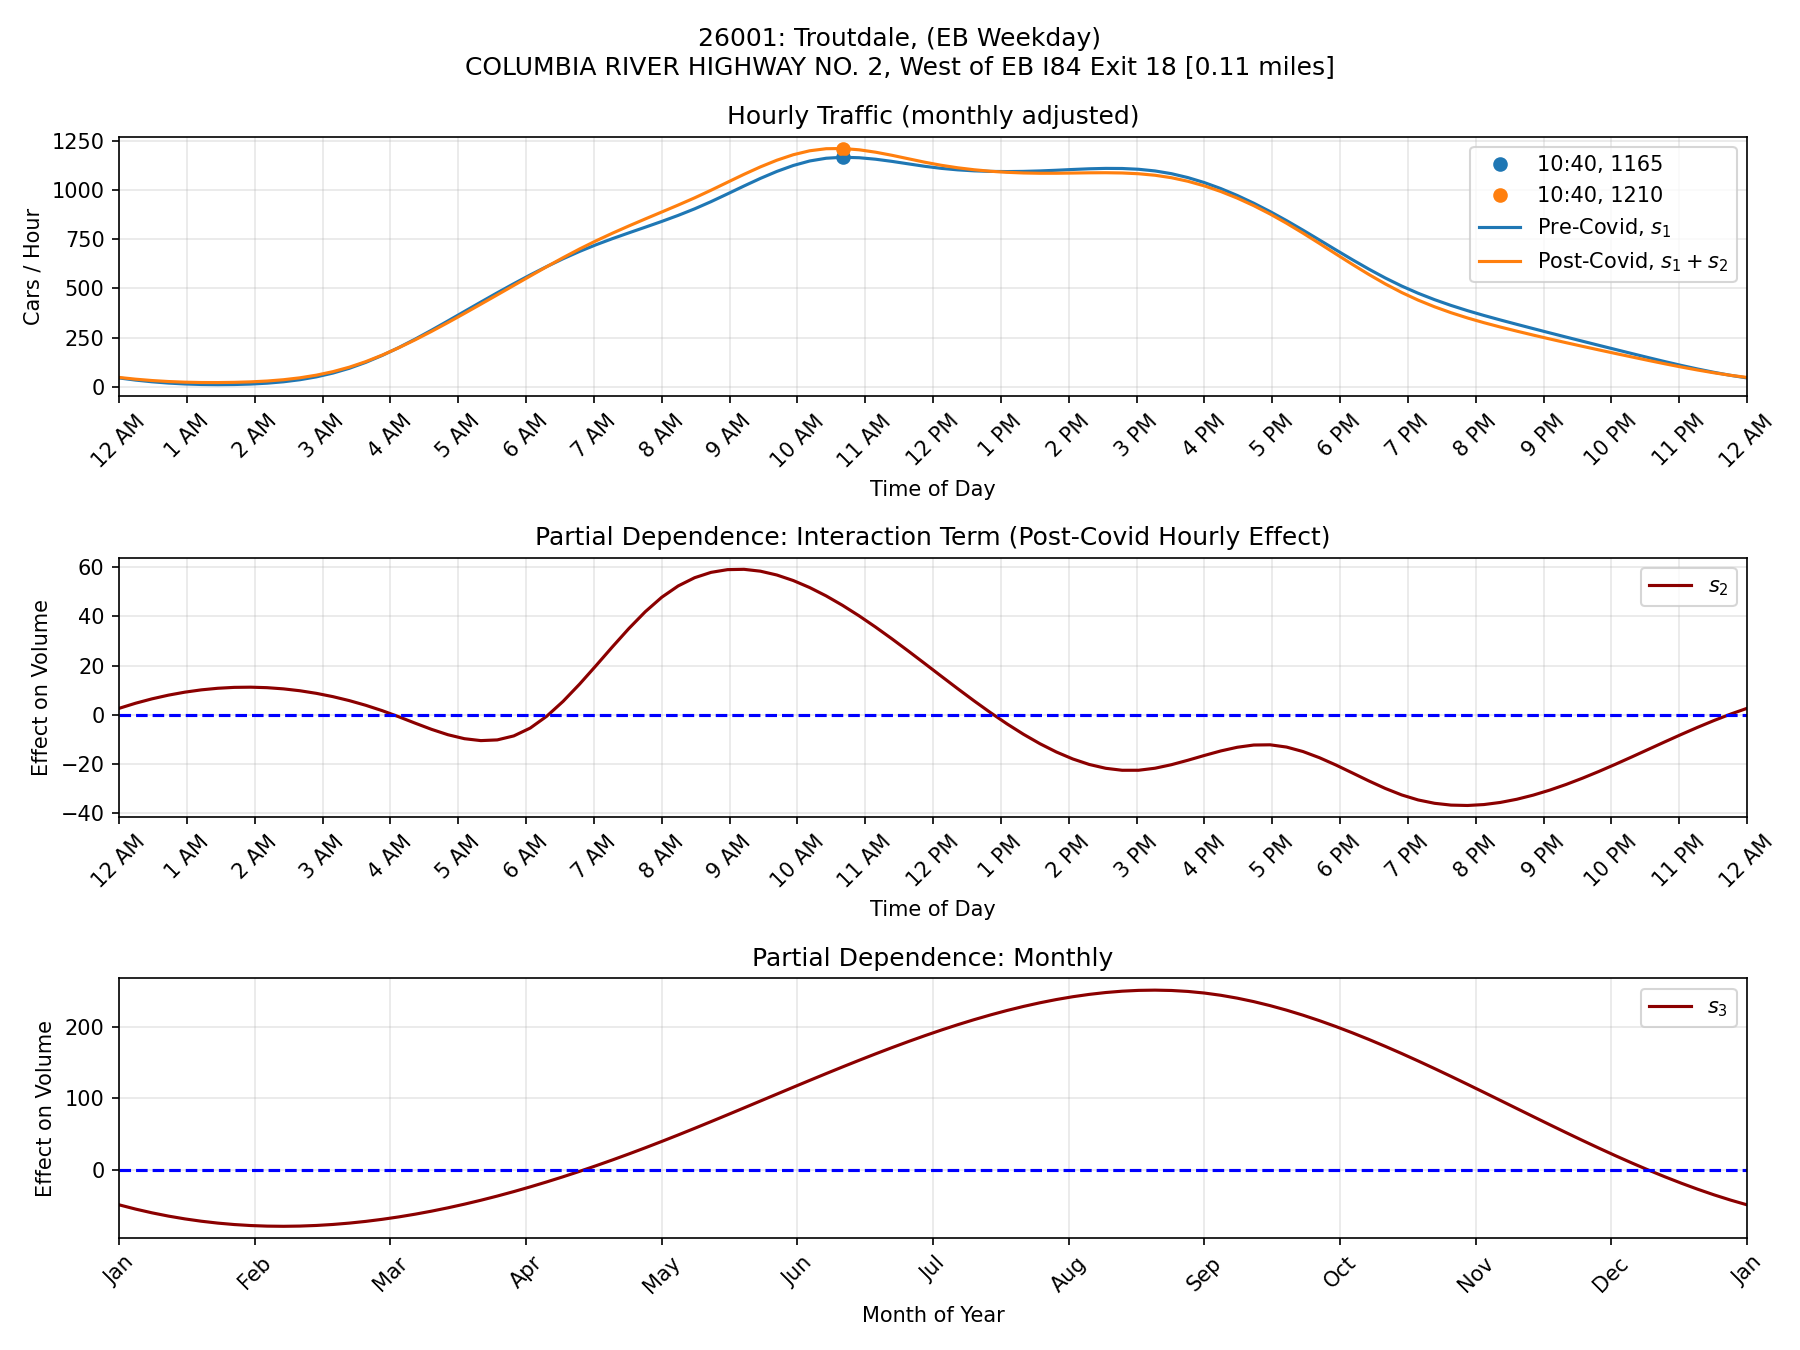
\includegraphics[width=\textwidth]{26001_Troutdale_EB_Weekday_gam.png}
	\end{subfigure}
	\hfill
	\begin{subfigure}[b]{0.45\textwidth}
		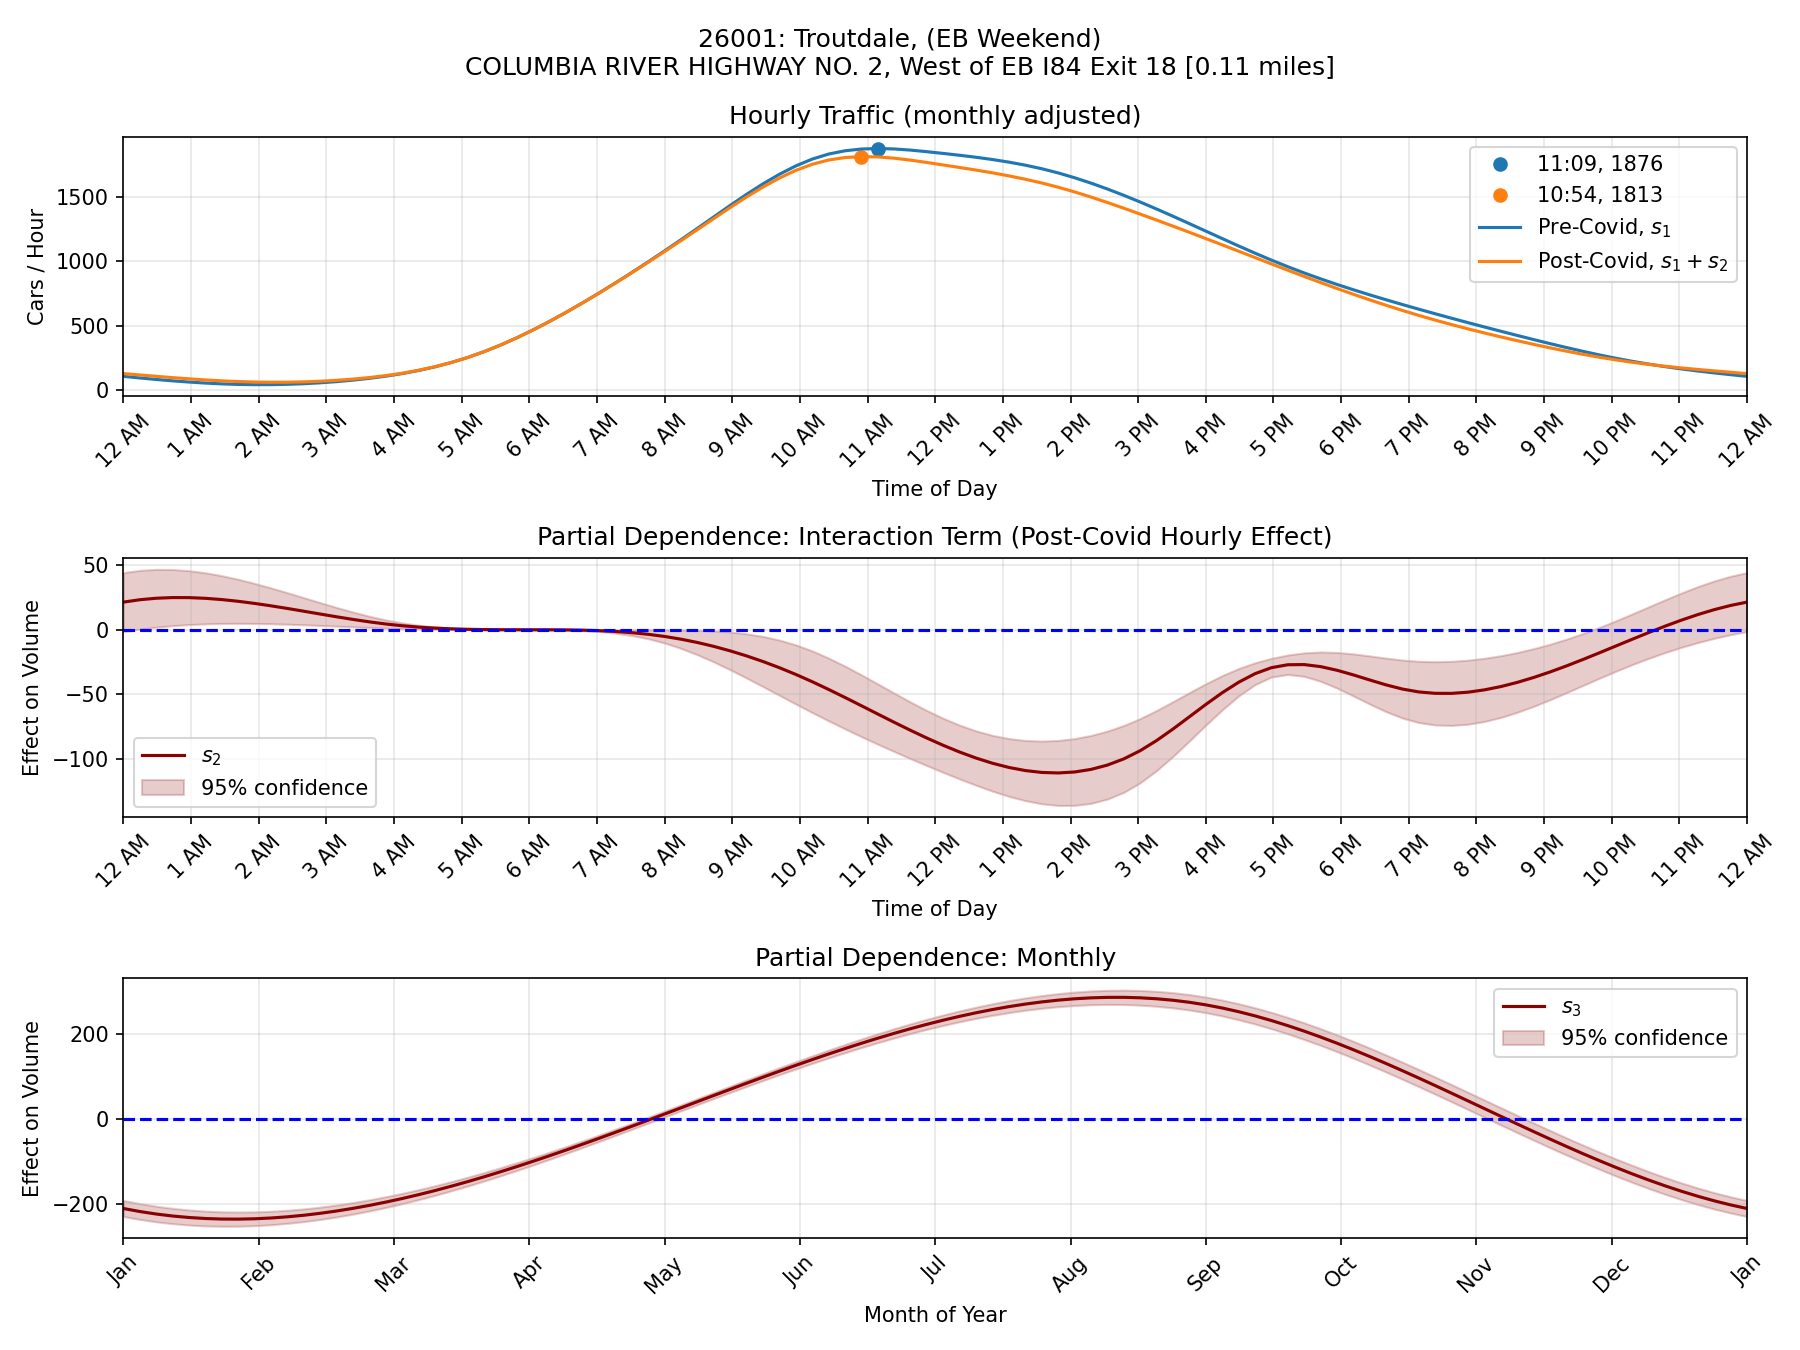
\includegraphics[width=\textwidth]{26001_Troutdale_EB_Weekend_gam.png}
	\end{subfigure}

	\begin{subfigure}[b]{0.45\textwidth}
		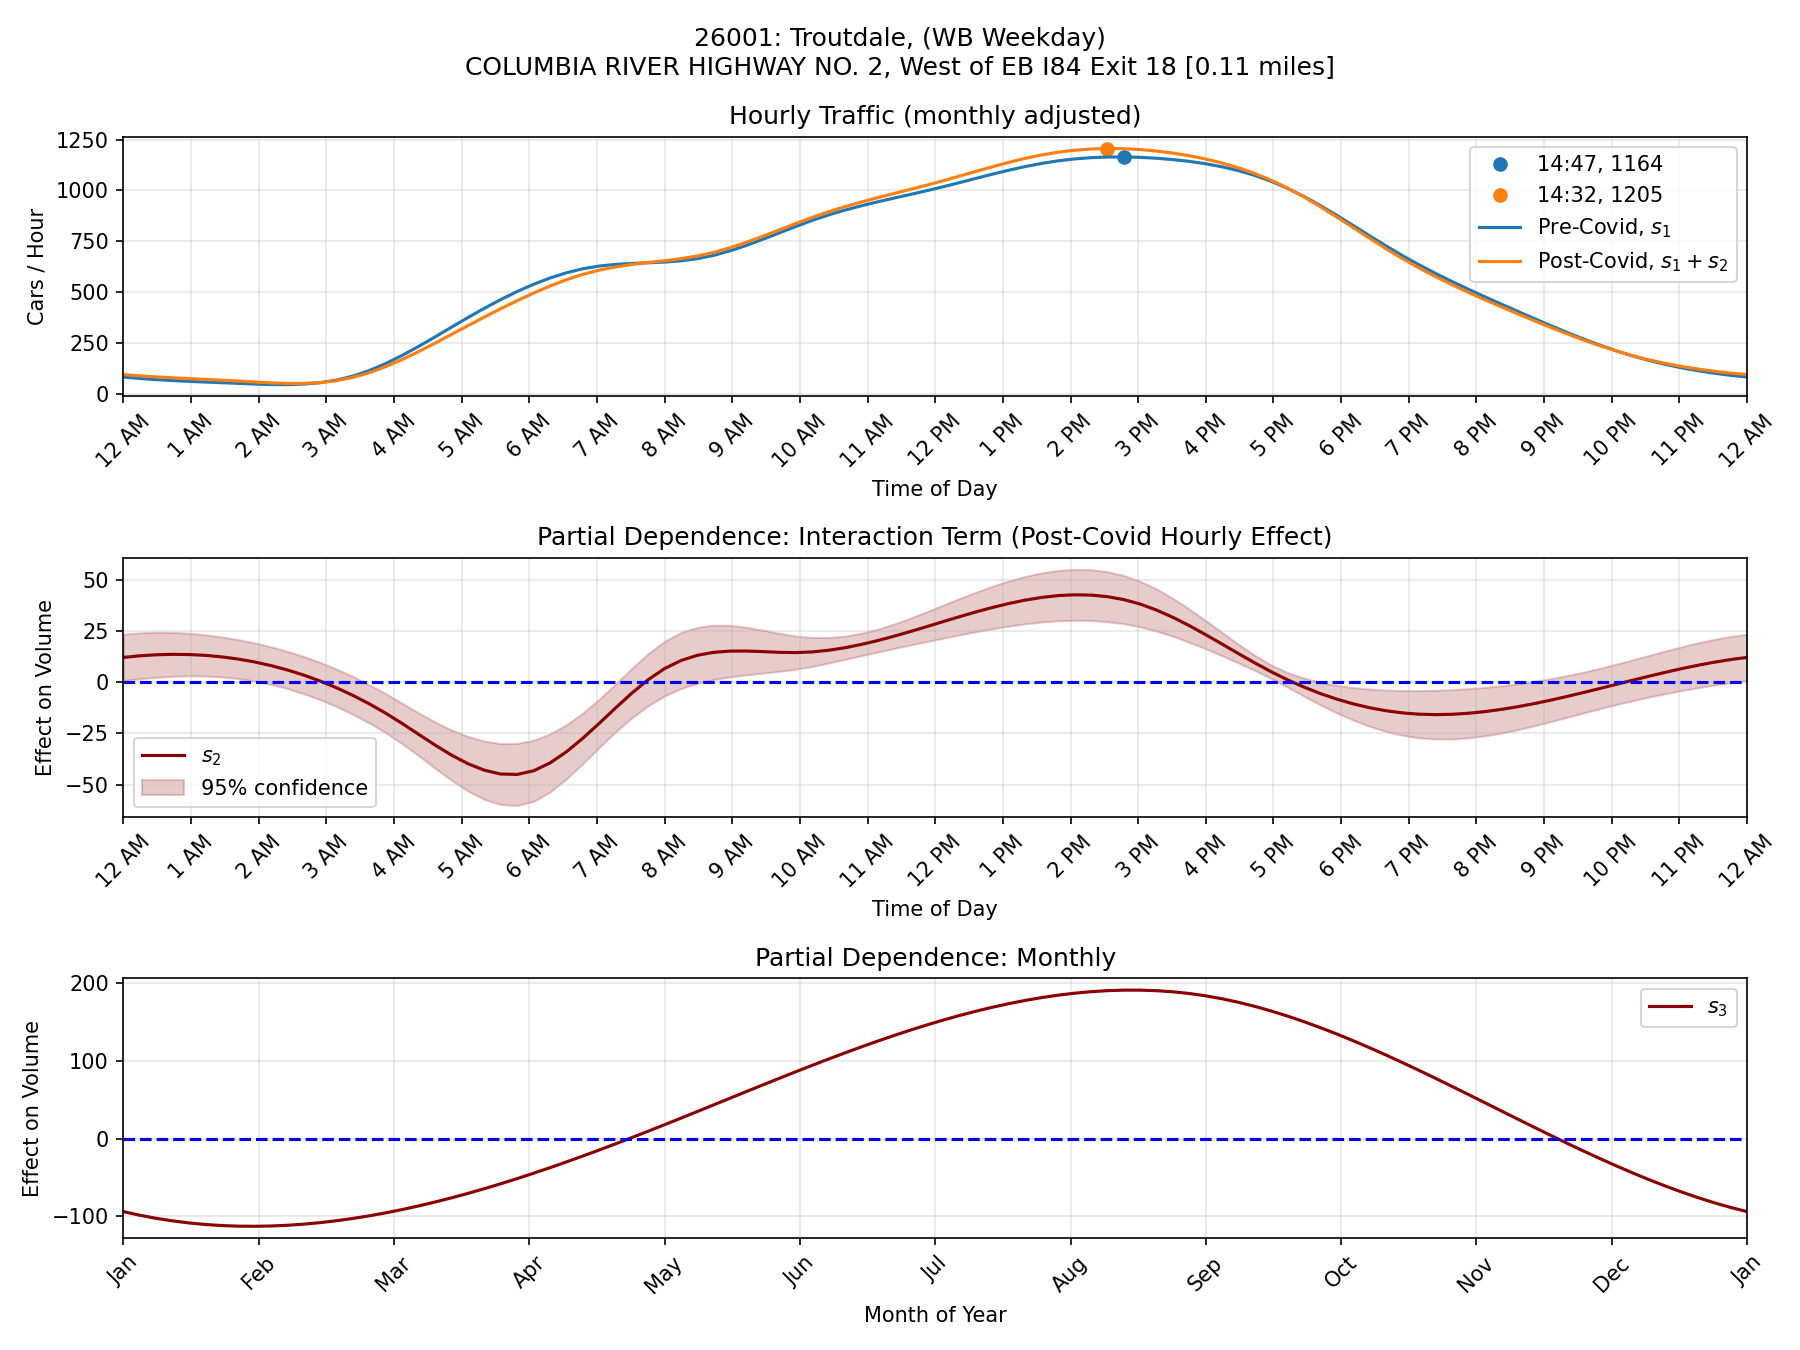
\includegraphics[width=\textwidth]{26001_Troutdale_WB_Weekday_gam.png}
	\end{subfigure}
	\hfill
	\begin{subfigure}[b]{0.45\textwidth}
		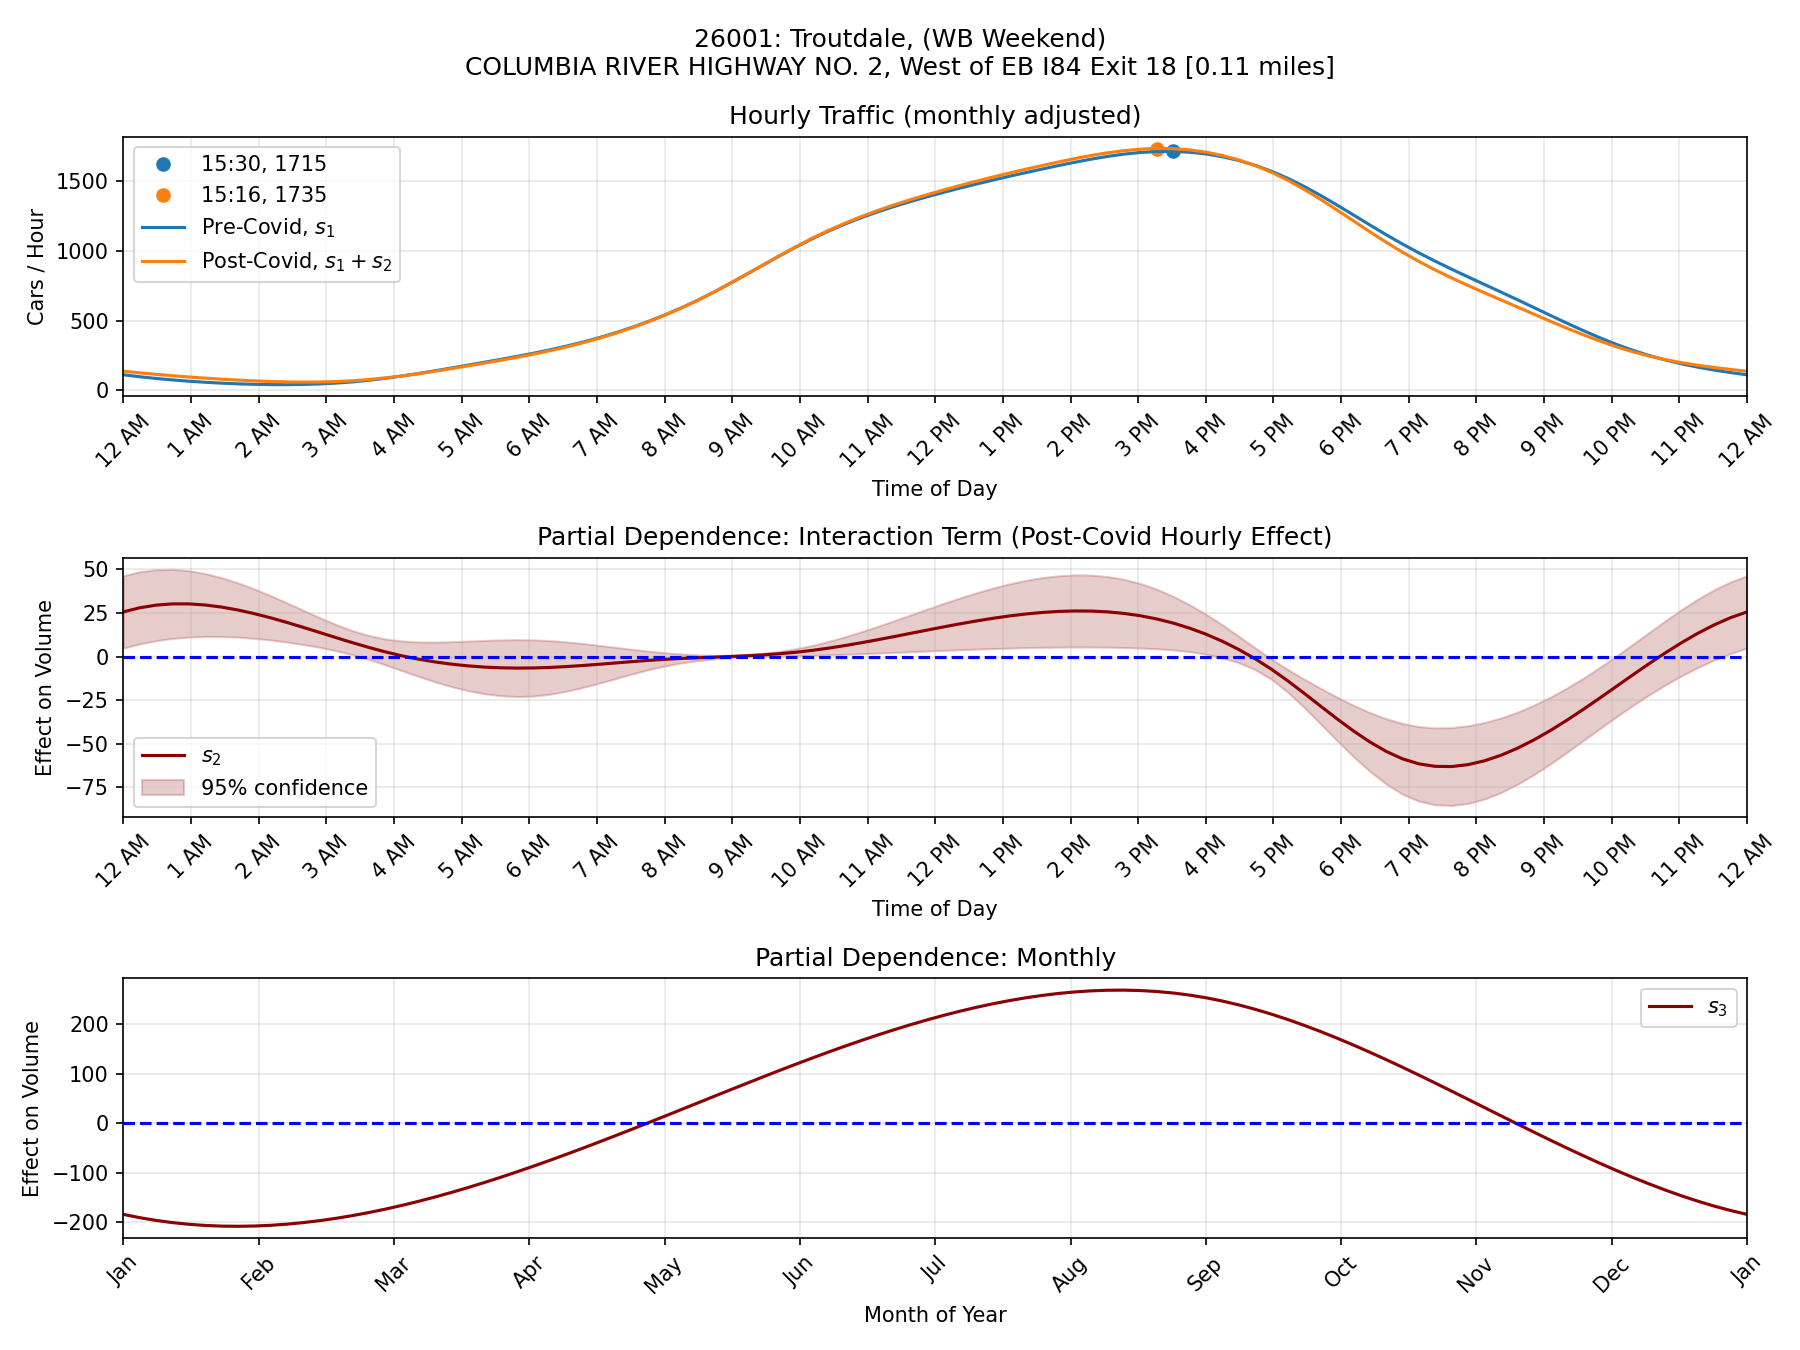
\includegraphics[width=\textwidth]{26001_Troutdale_WB_Weekend_gam.png}
	\end{subfigure}
\end{figure}

\begin{figure}[H]
	\centering
	\begin{subfigure}[b]{0.45\textwidth}
		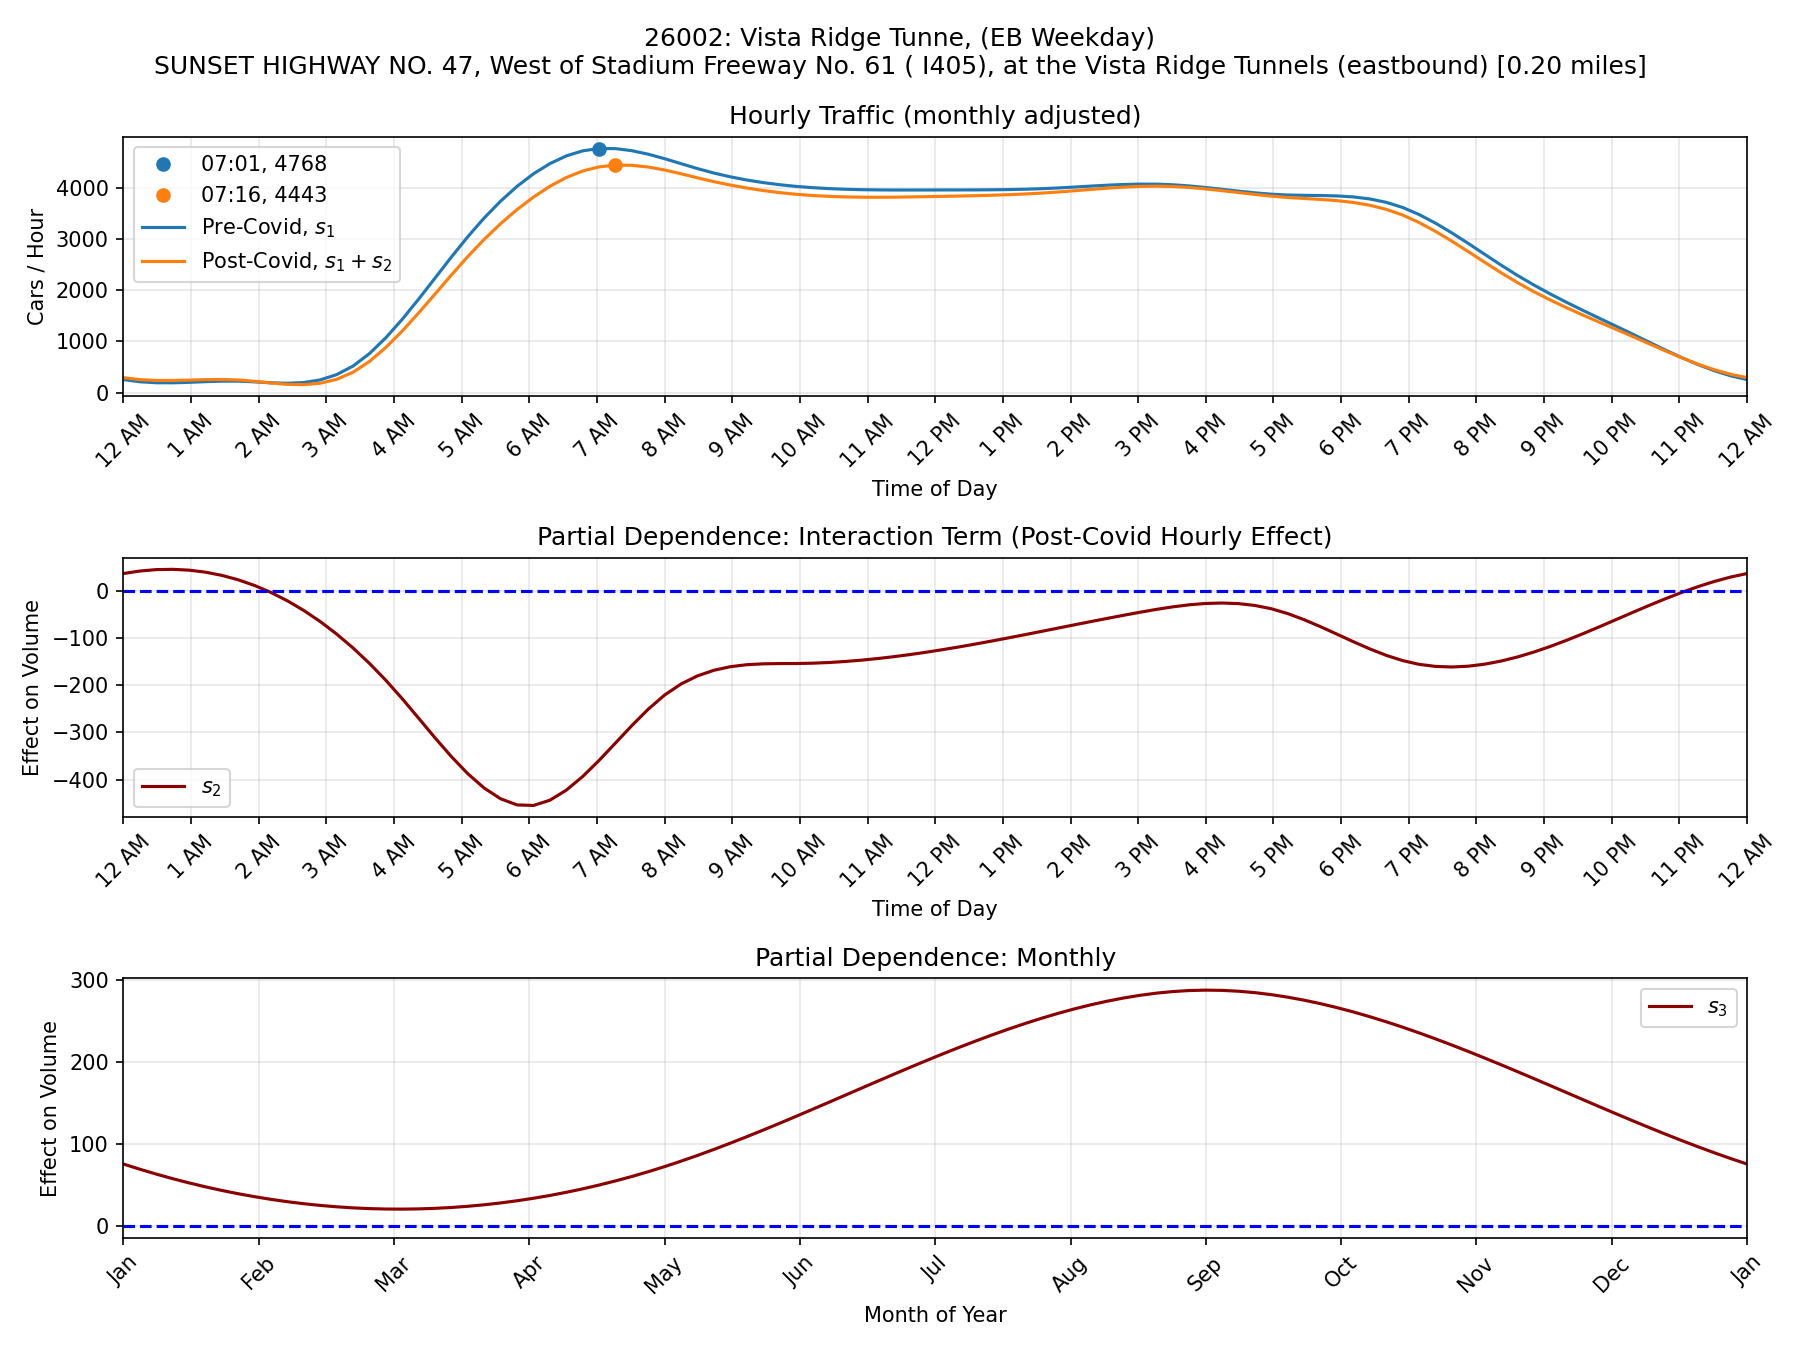
\includegraphics[width=\textwidth]{26002_Vista-Ridge-Tunne_EB_Weekday_gam.png}
	\end{subfigure}
	\hfill
	\begin{subfigure}[b]{0.45\textwidth}
		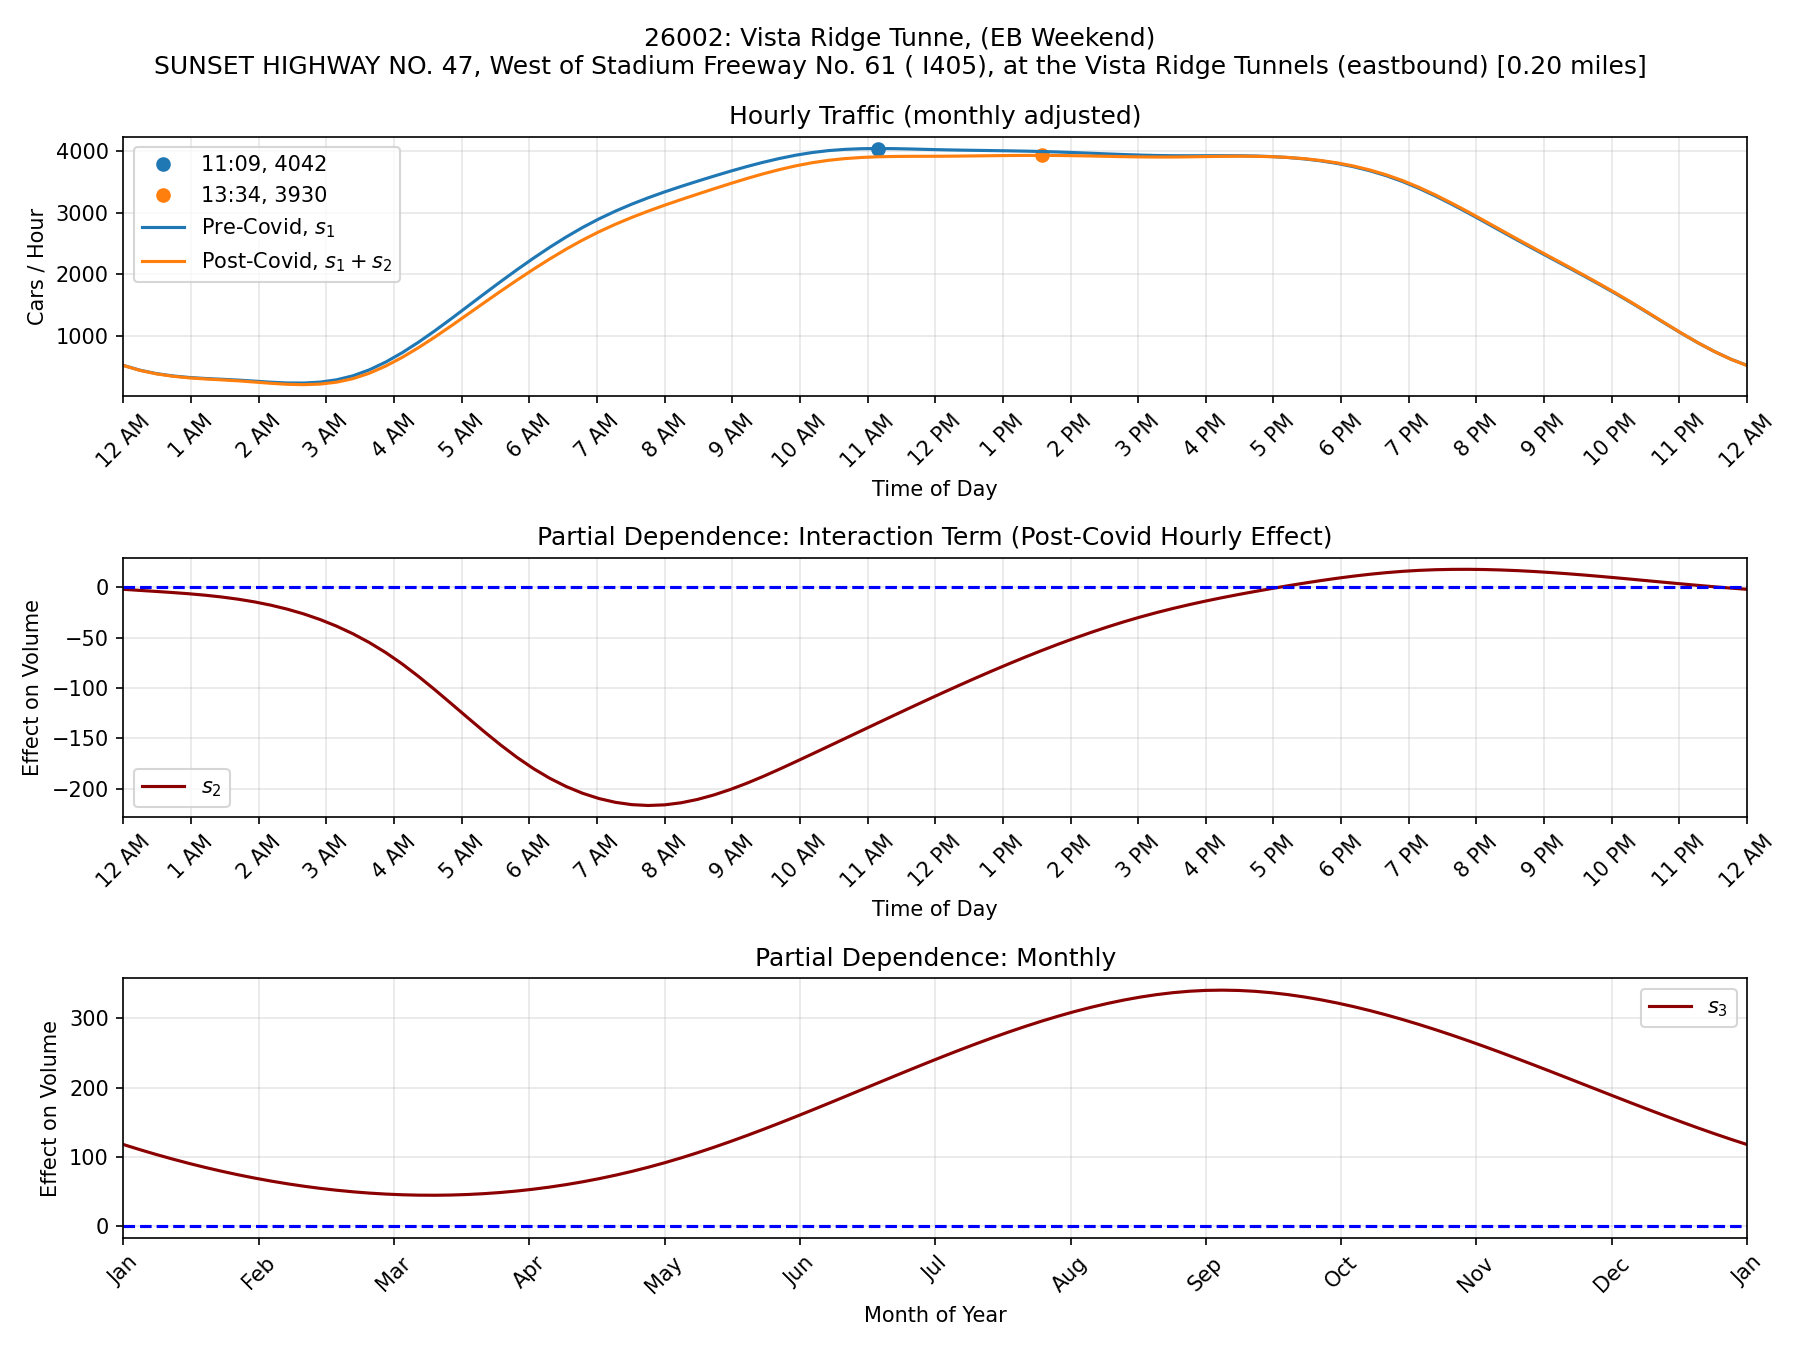
\includegraphics[width=\textwidth]{26002_Vista-Ridge-Tunne_EB_Weekend_gam.png}
	\end{subfigure}

	\begin{subfigure}[b]{0.45\textwidth}
		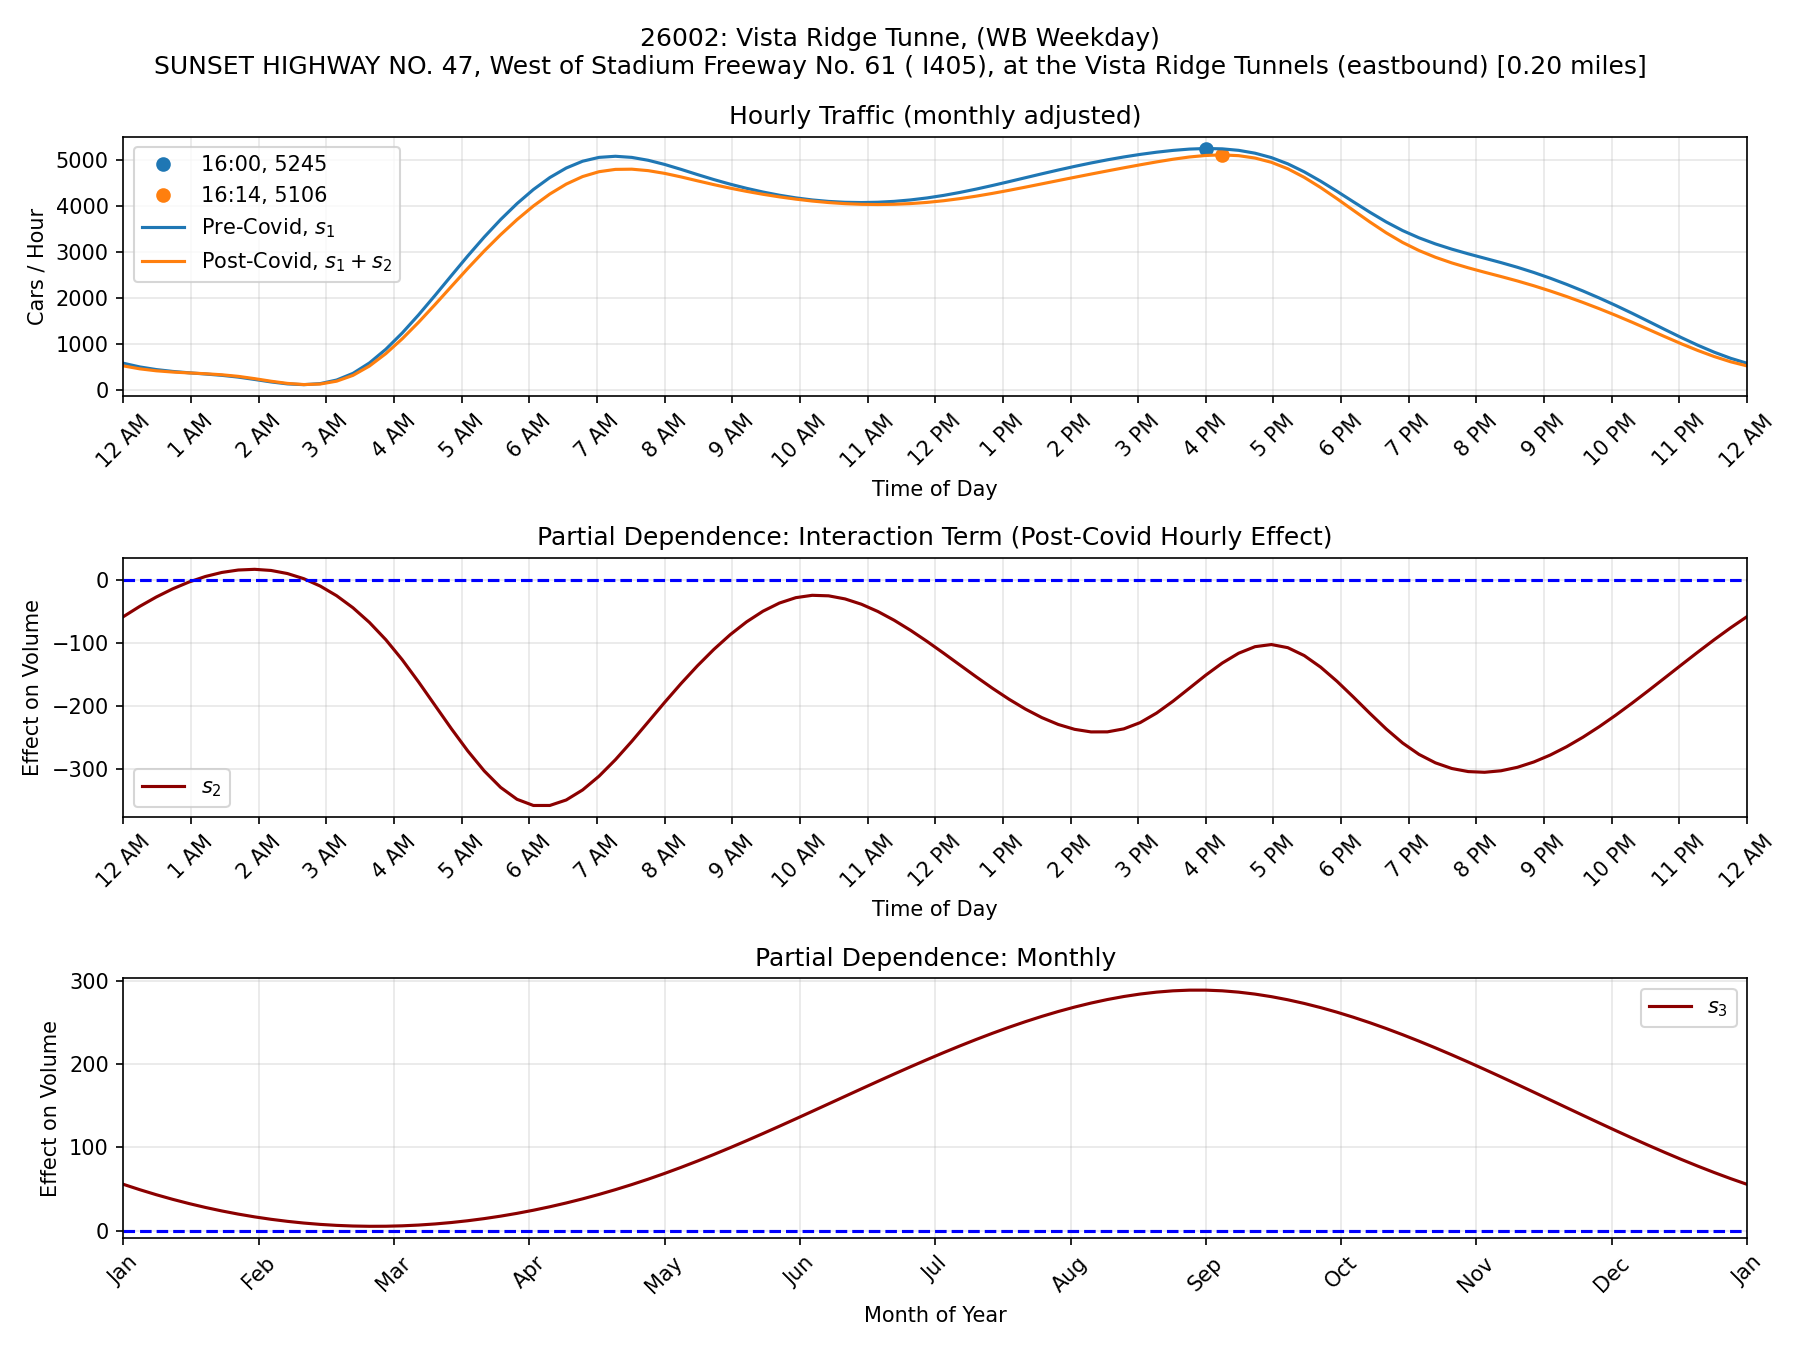
\includegraphics[width=\textwidth]{26002_Vista-Ridge-Tunne_WB_Weekday_gam.png}
	\end{subfigure}
	\hfill
	\begin{subfigure}[b]{0.45\textwidth}
		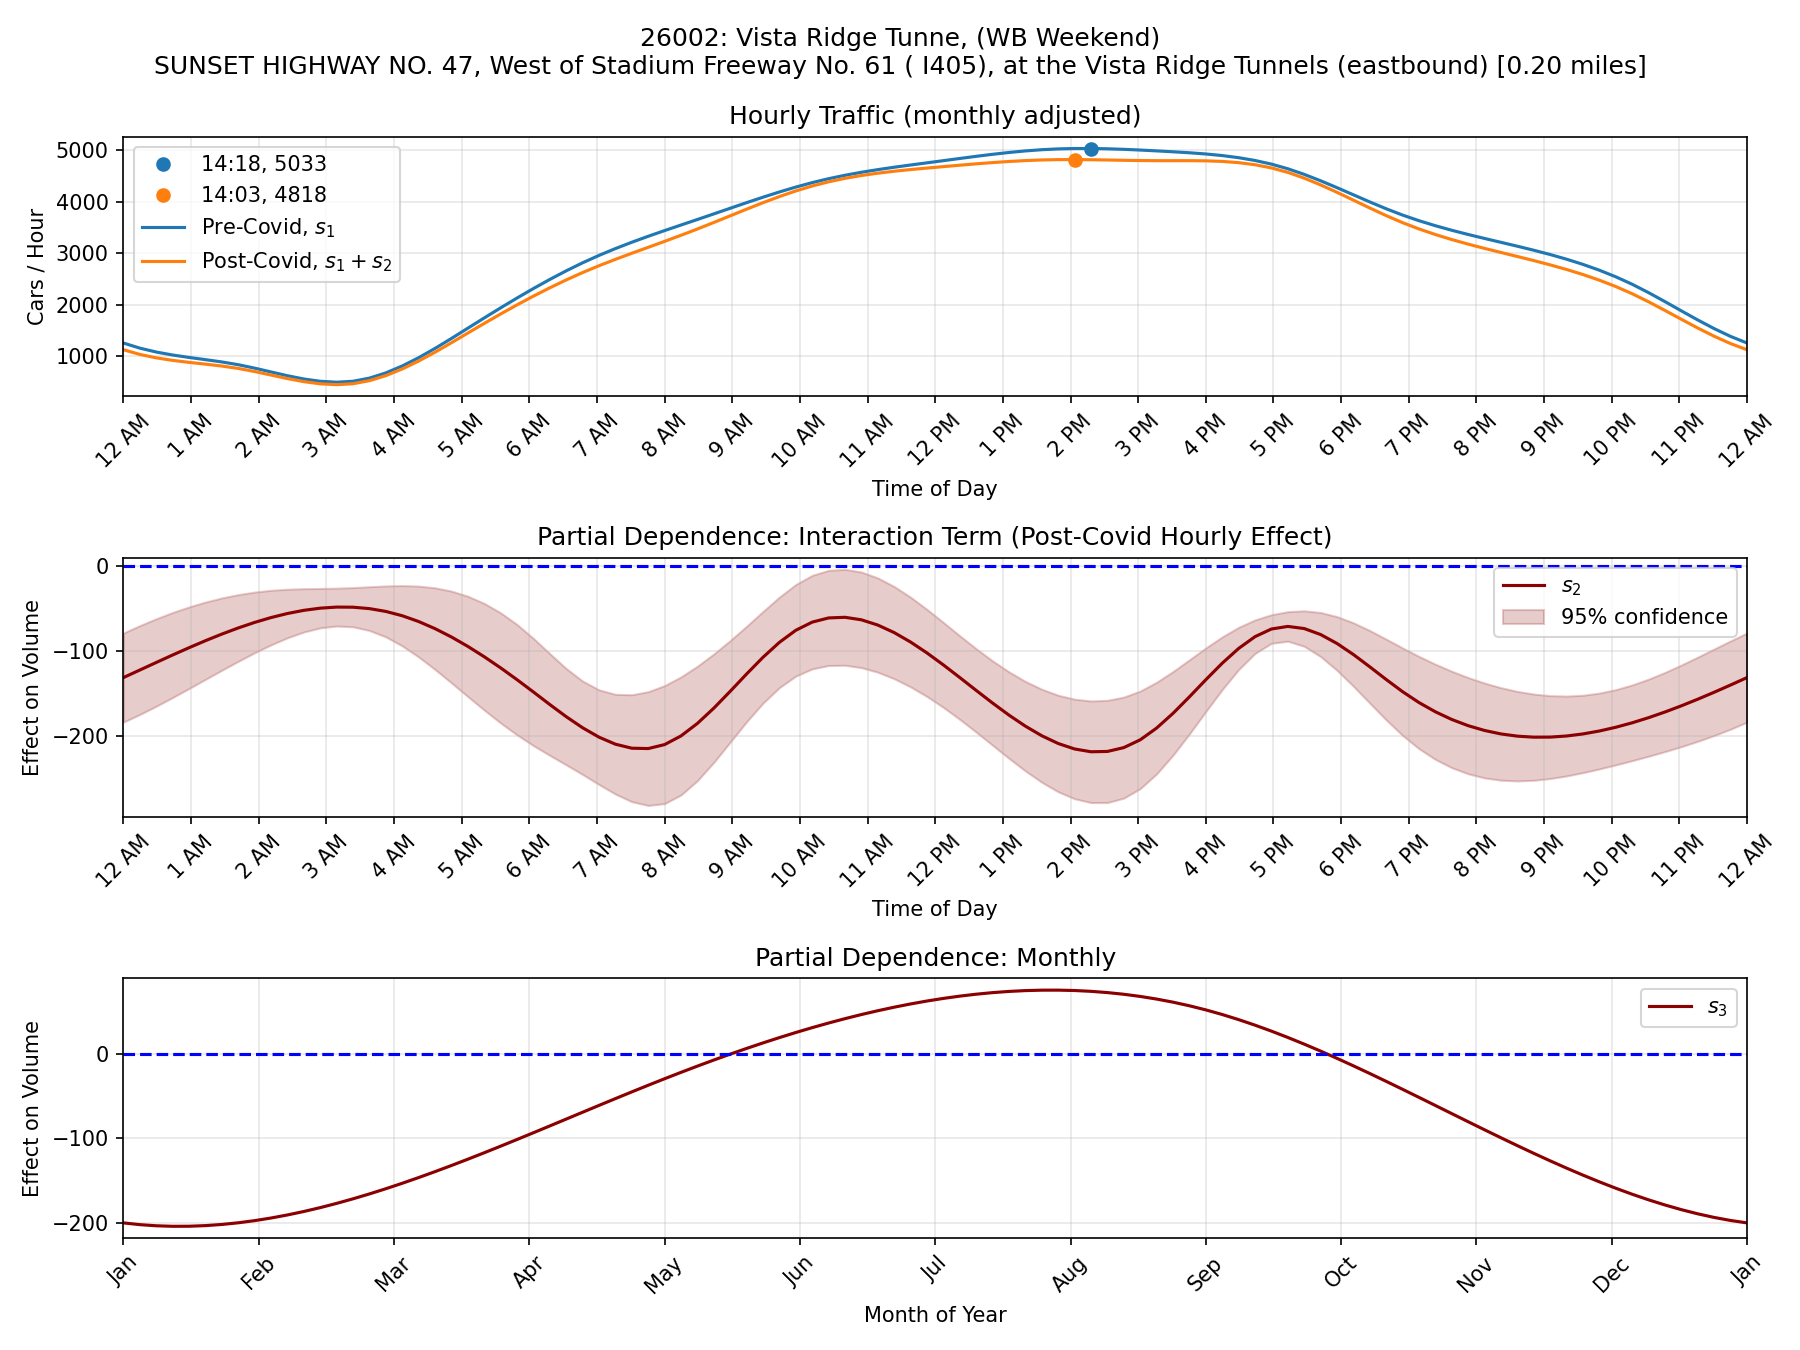
\includegraphics[width=\textwidth]{26002_Vista-Ridge-Tunne_WB_Weekend_gam.png}
	\end{subfigure}
\end{figure}

\begin{figure}[H]
	\centering
	\begin{subfigure}[b]{0.45\textwidth}
		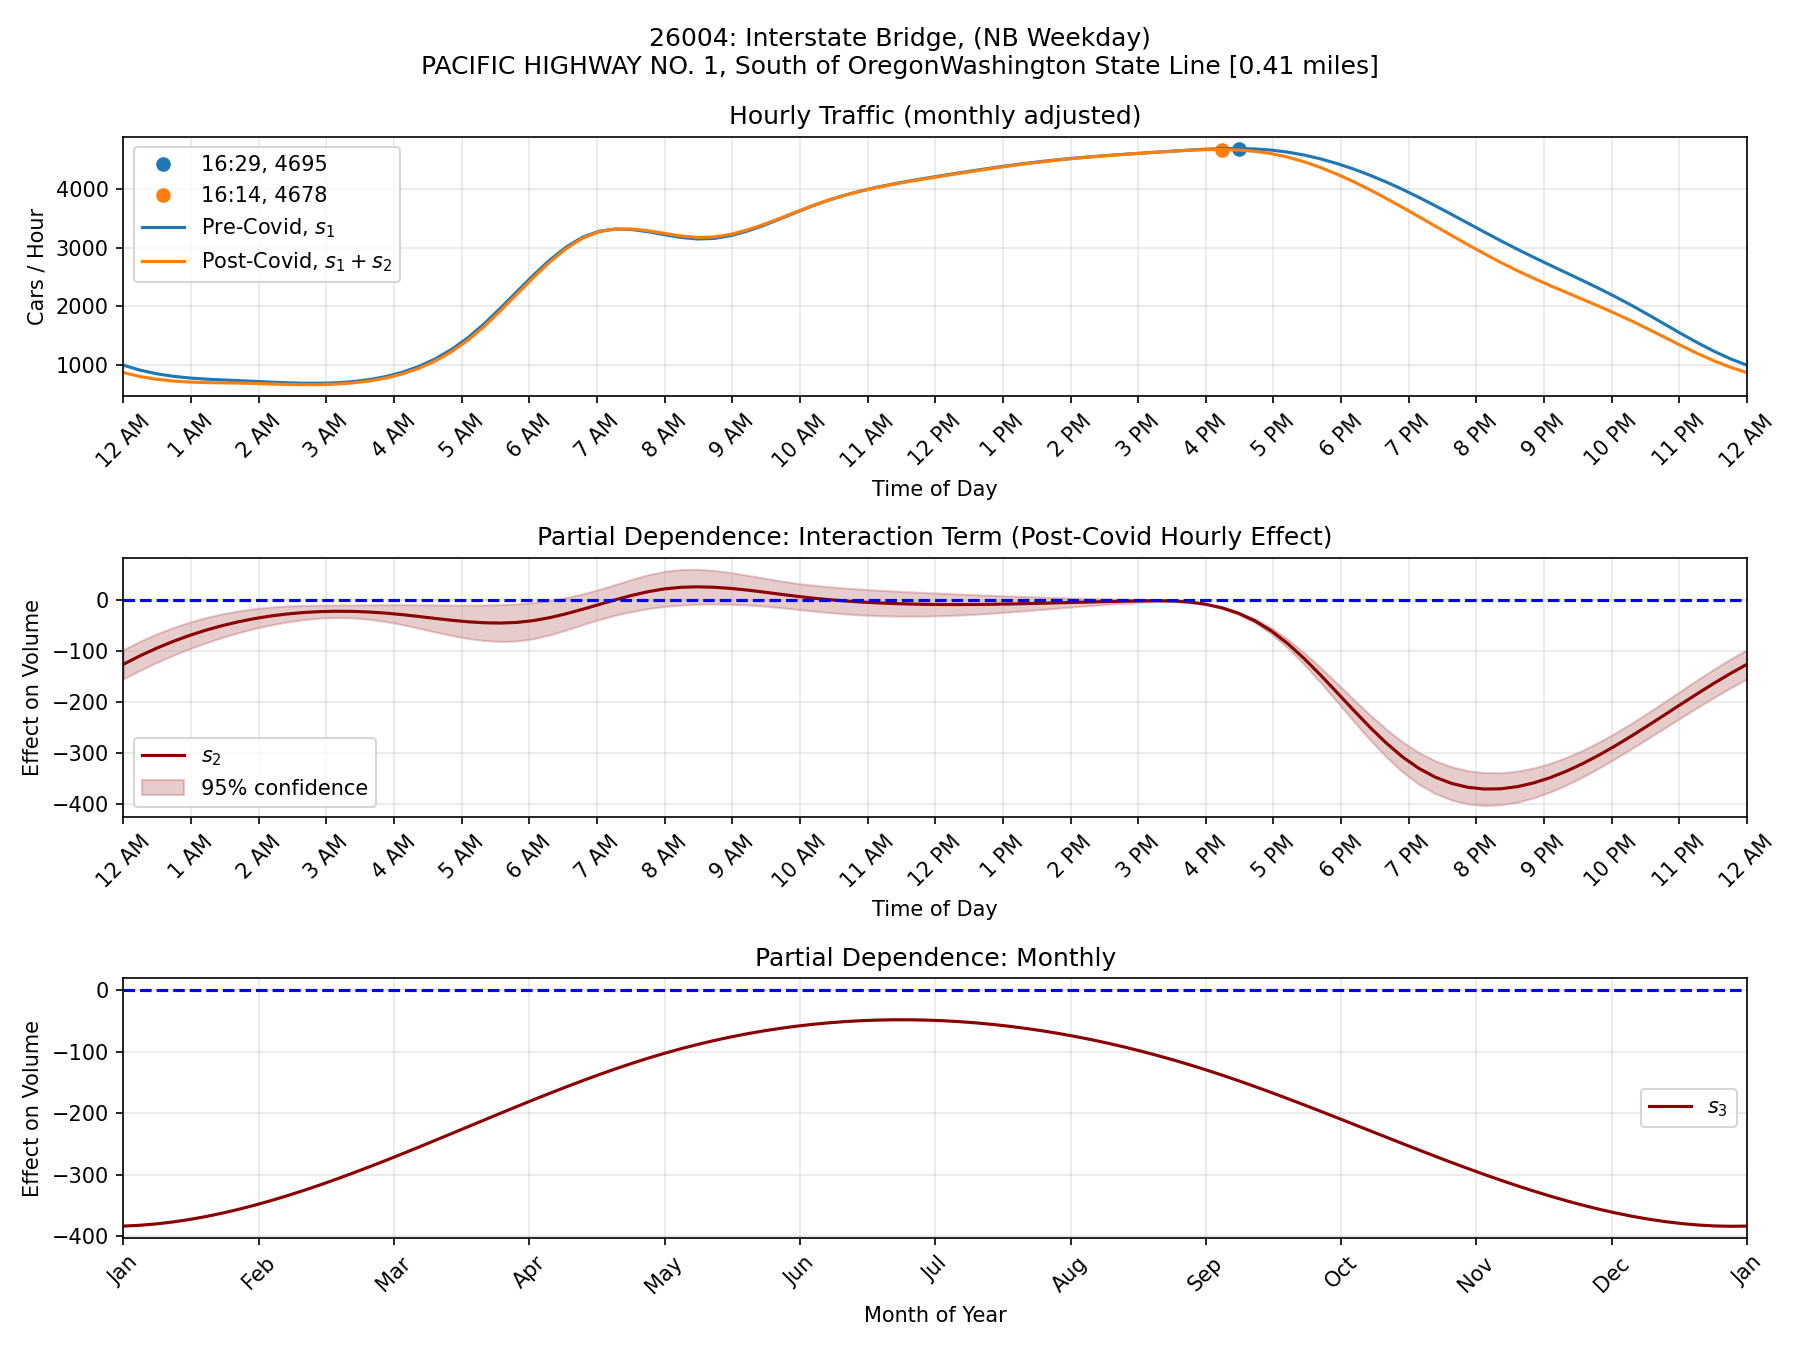
\includegraphics[width=\textwidth]{26004_Interstate-Bridge_NB_Weekday_gam.png}
	\end{subfigure}
	\hfill
	\begin{subfigure}[b]{0.45\textwidth}
		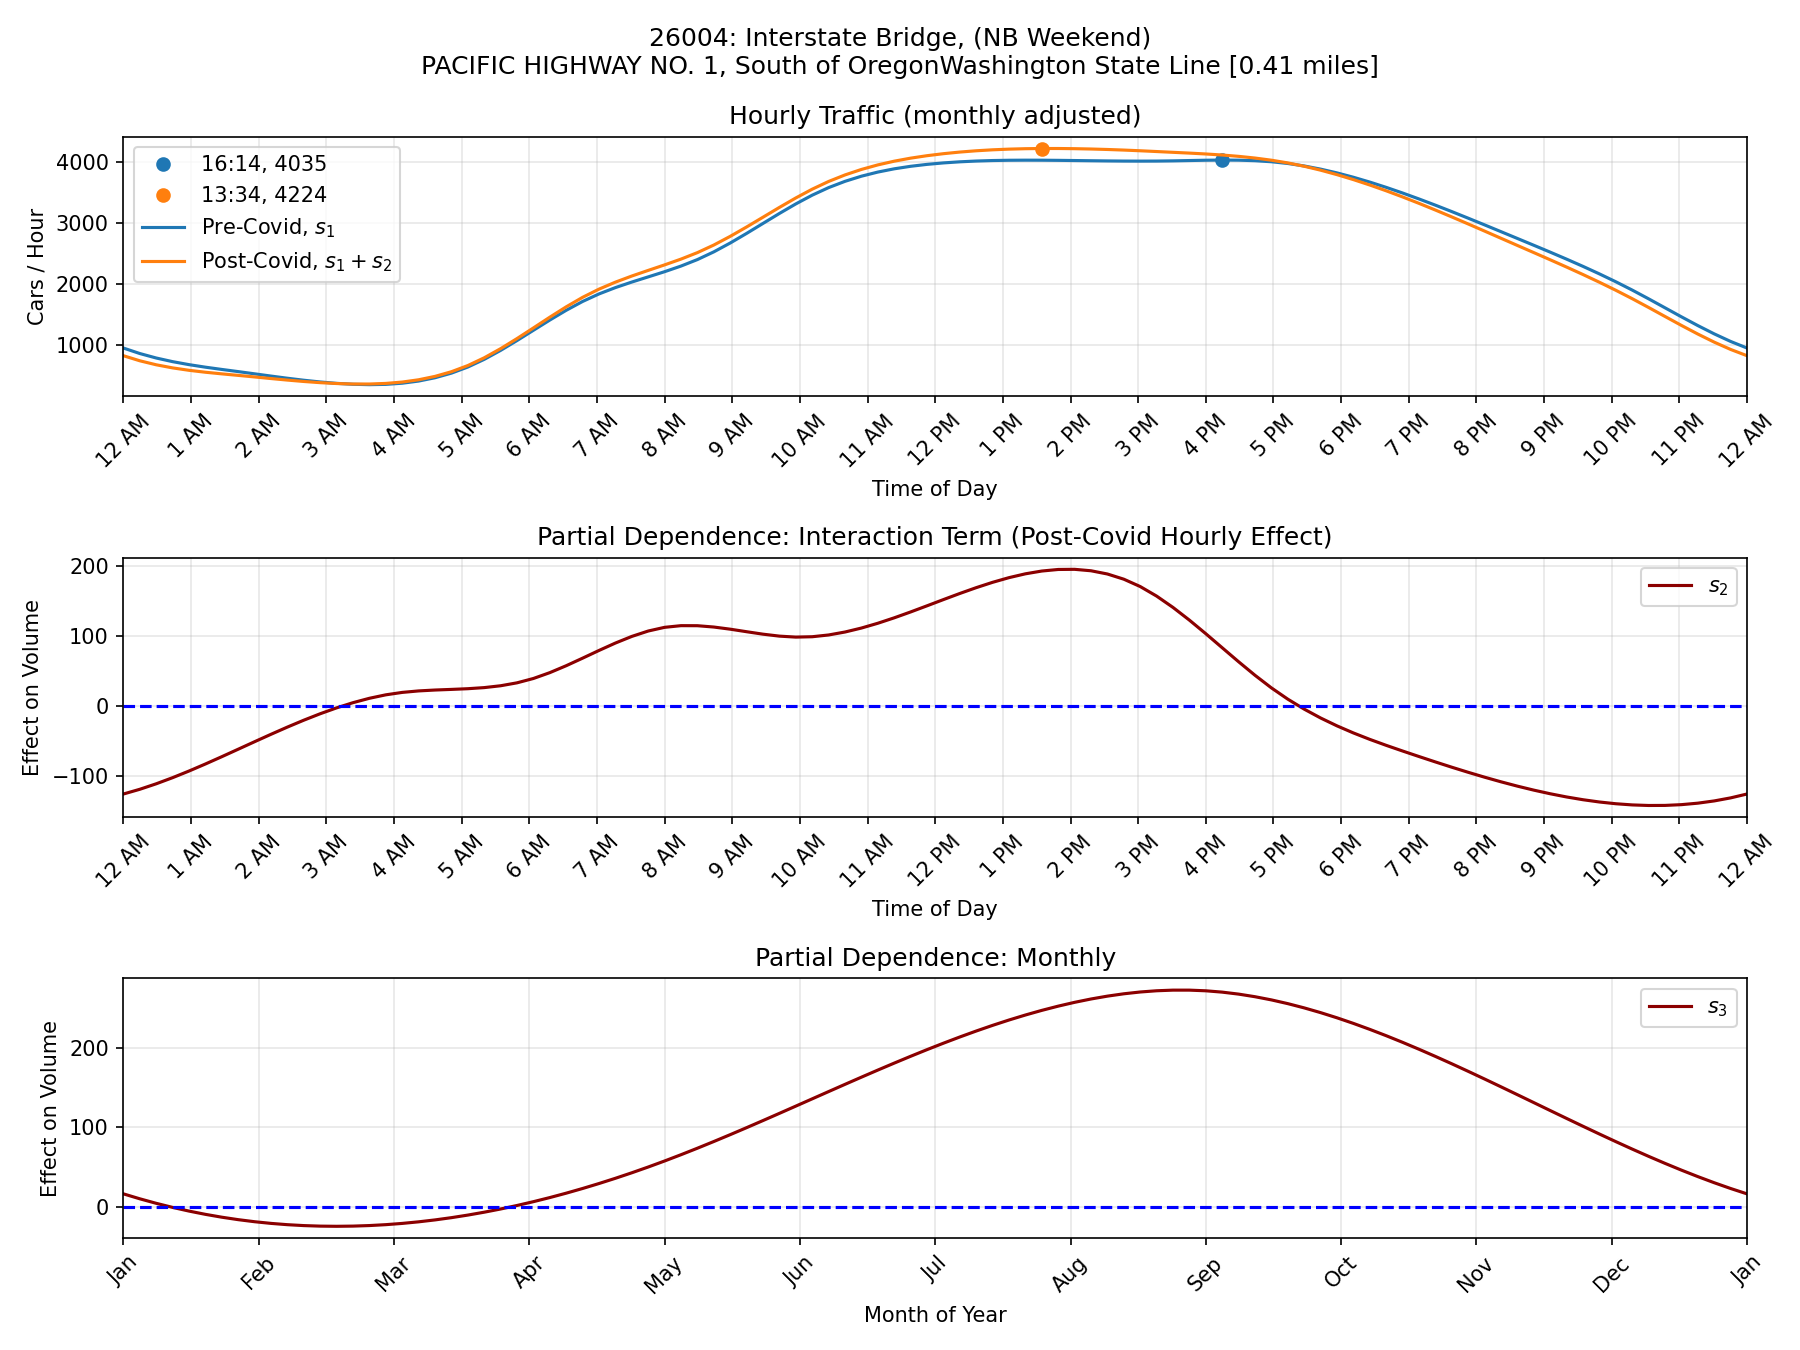
\includegraphics[width=\textwidth]{26004_Interstate-Bridge_NB_Weekend_gam.png}
	\end{subfigure}

	\begin{subfigure}[b]{0.45\textwidth}
		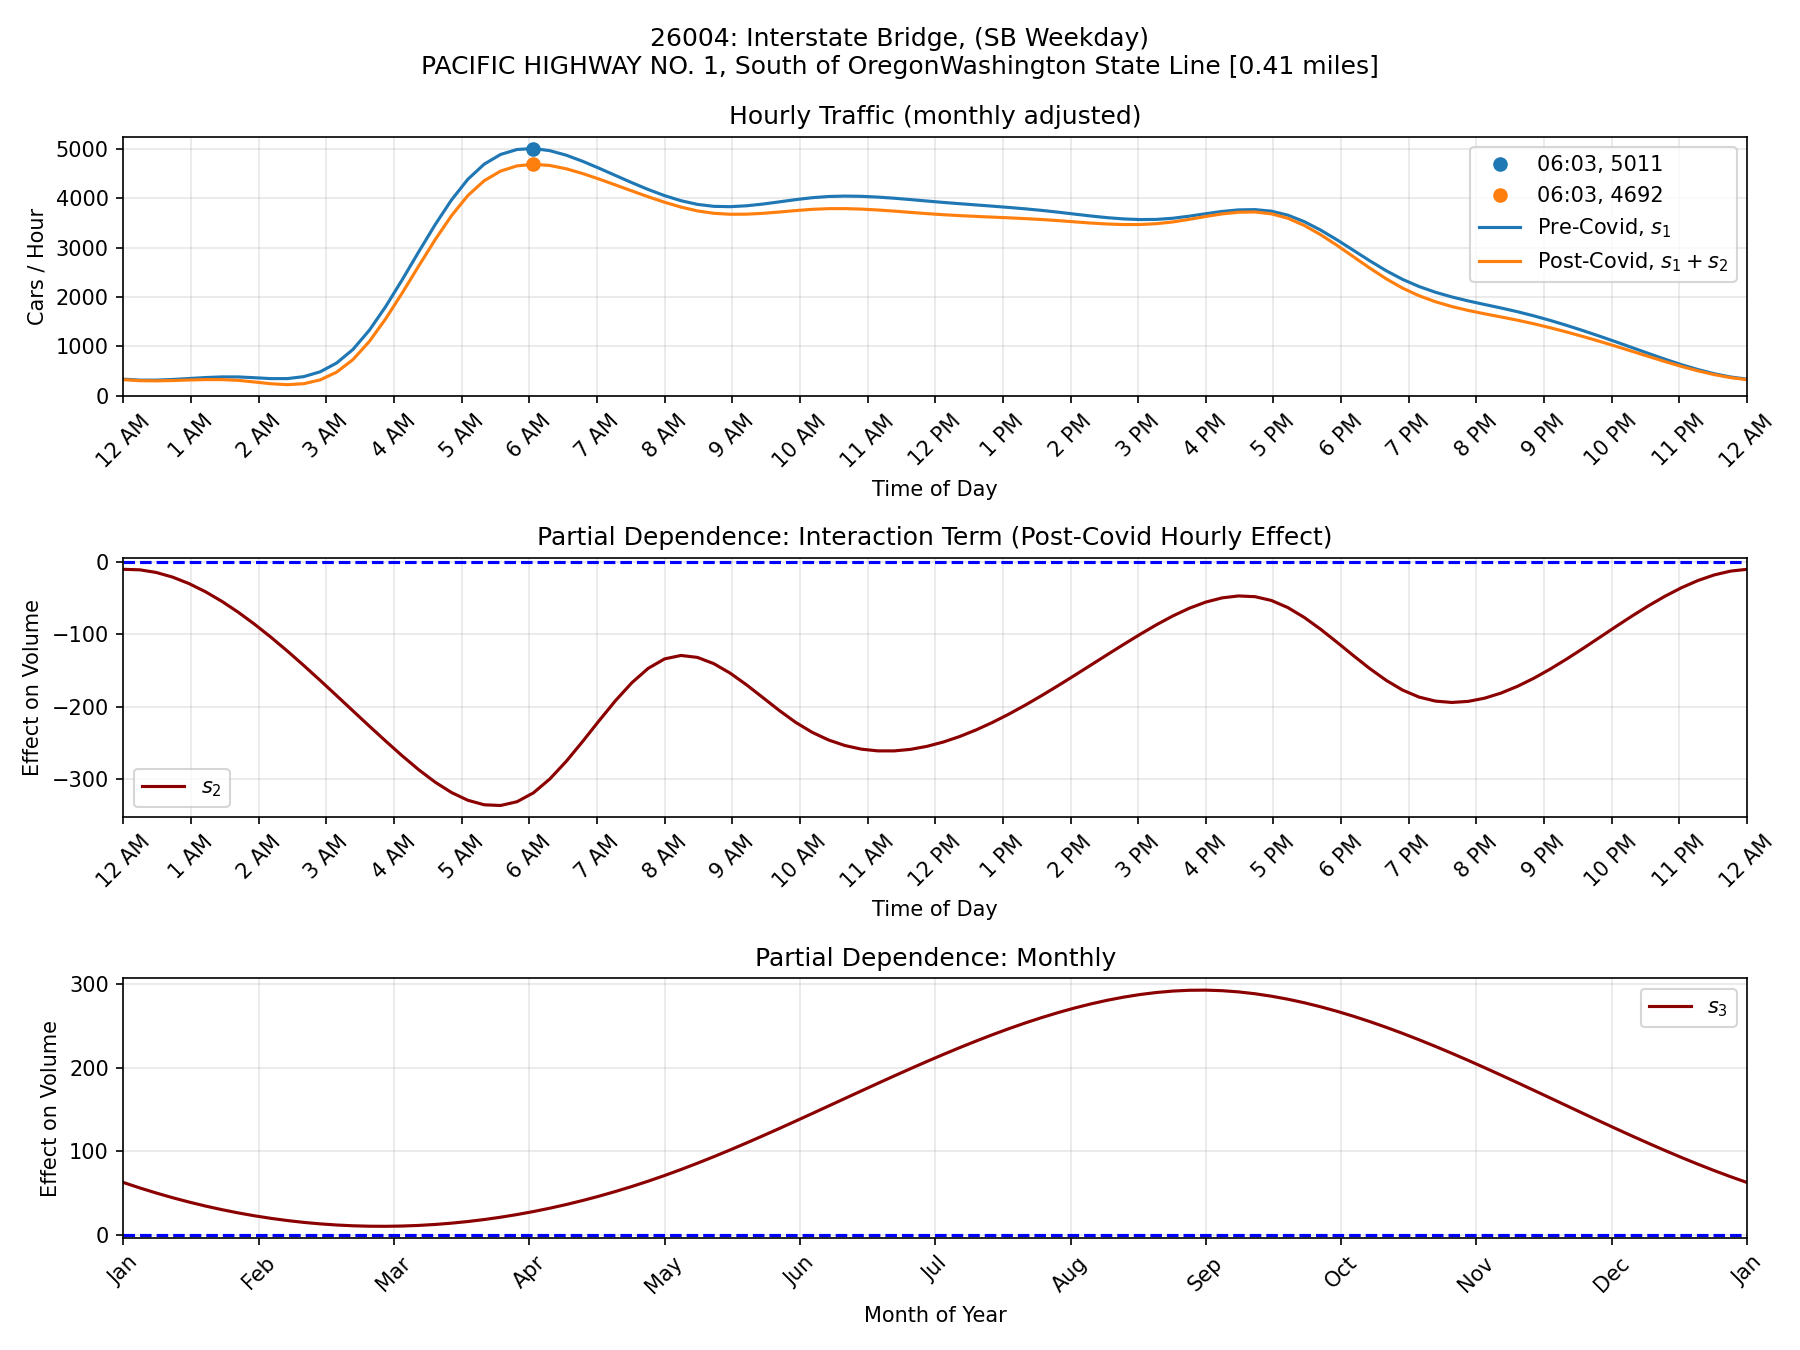
\includegraphics[width=\textwidth]{26004_Interstate-Bridge_SB_Weekday_gam.png}
	\end{subfigure}
	\hfill
	\begin{subfigure}[b]{0.45\textwidth}
		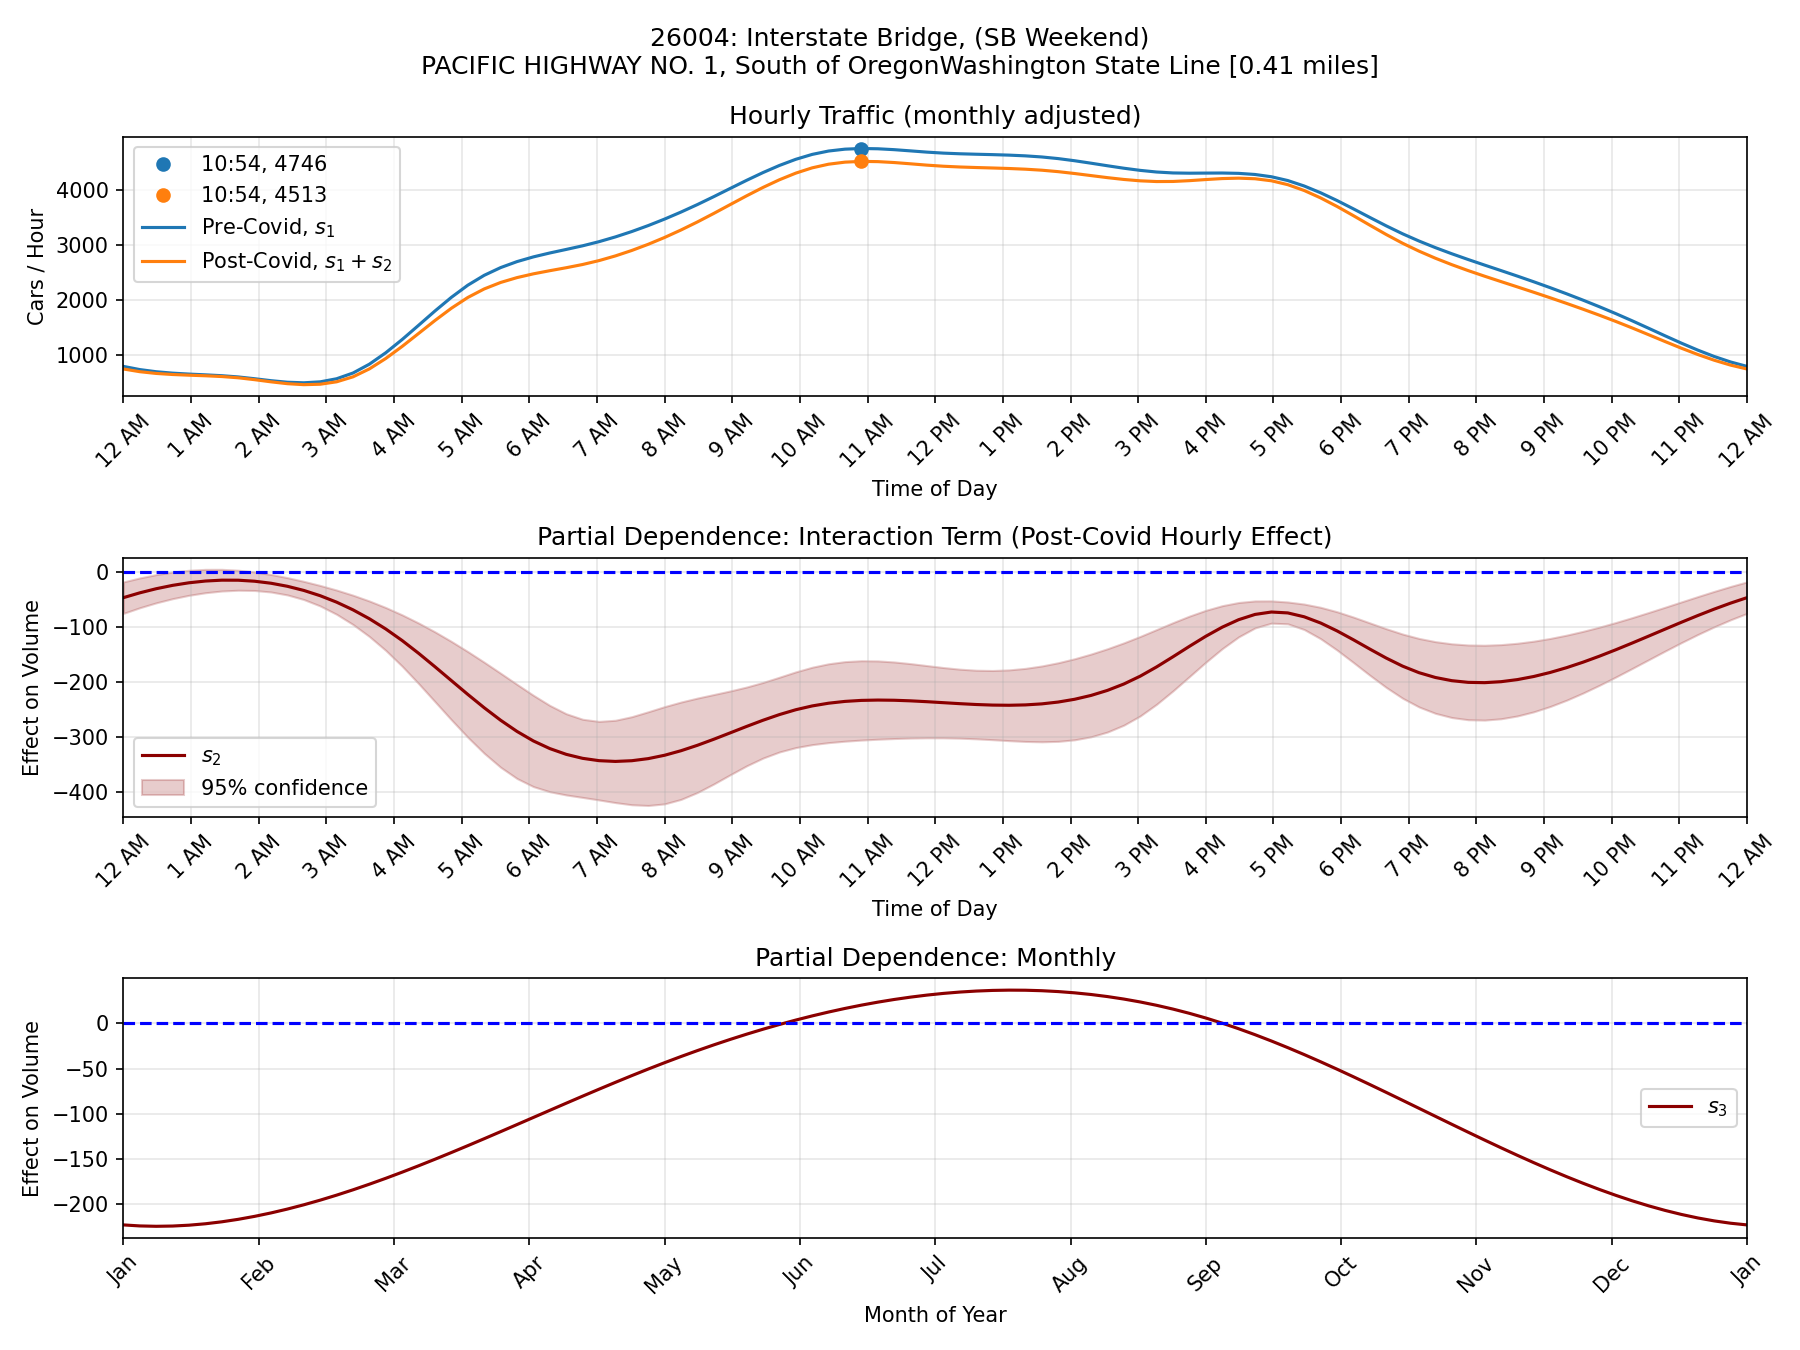
\includegraphics[width=\textwidth]{26004_Interstate-Bridge_SB_Weekend_gam.png}
	\end{subfigure}
\end{figure}

\begin{figure}[H]
	\centering
	\begin{subfigure}[b]{0.45\textwidth}
		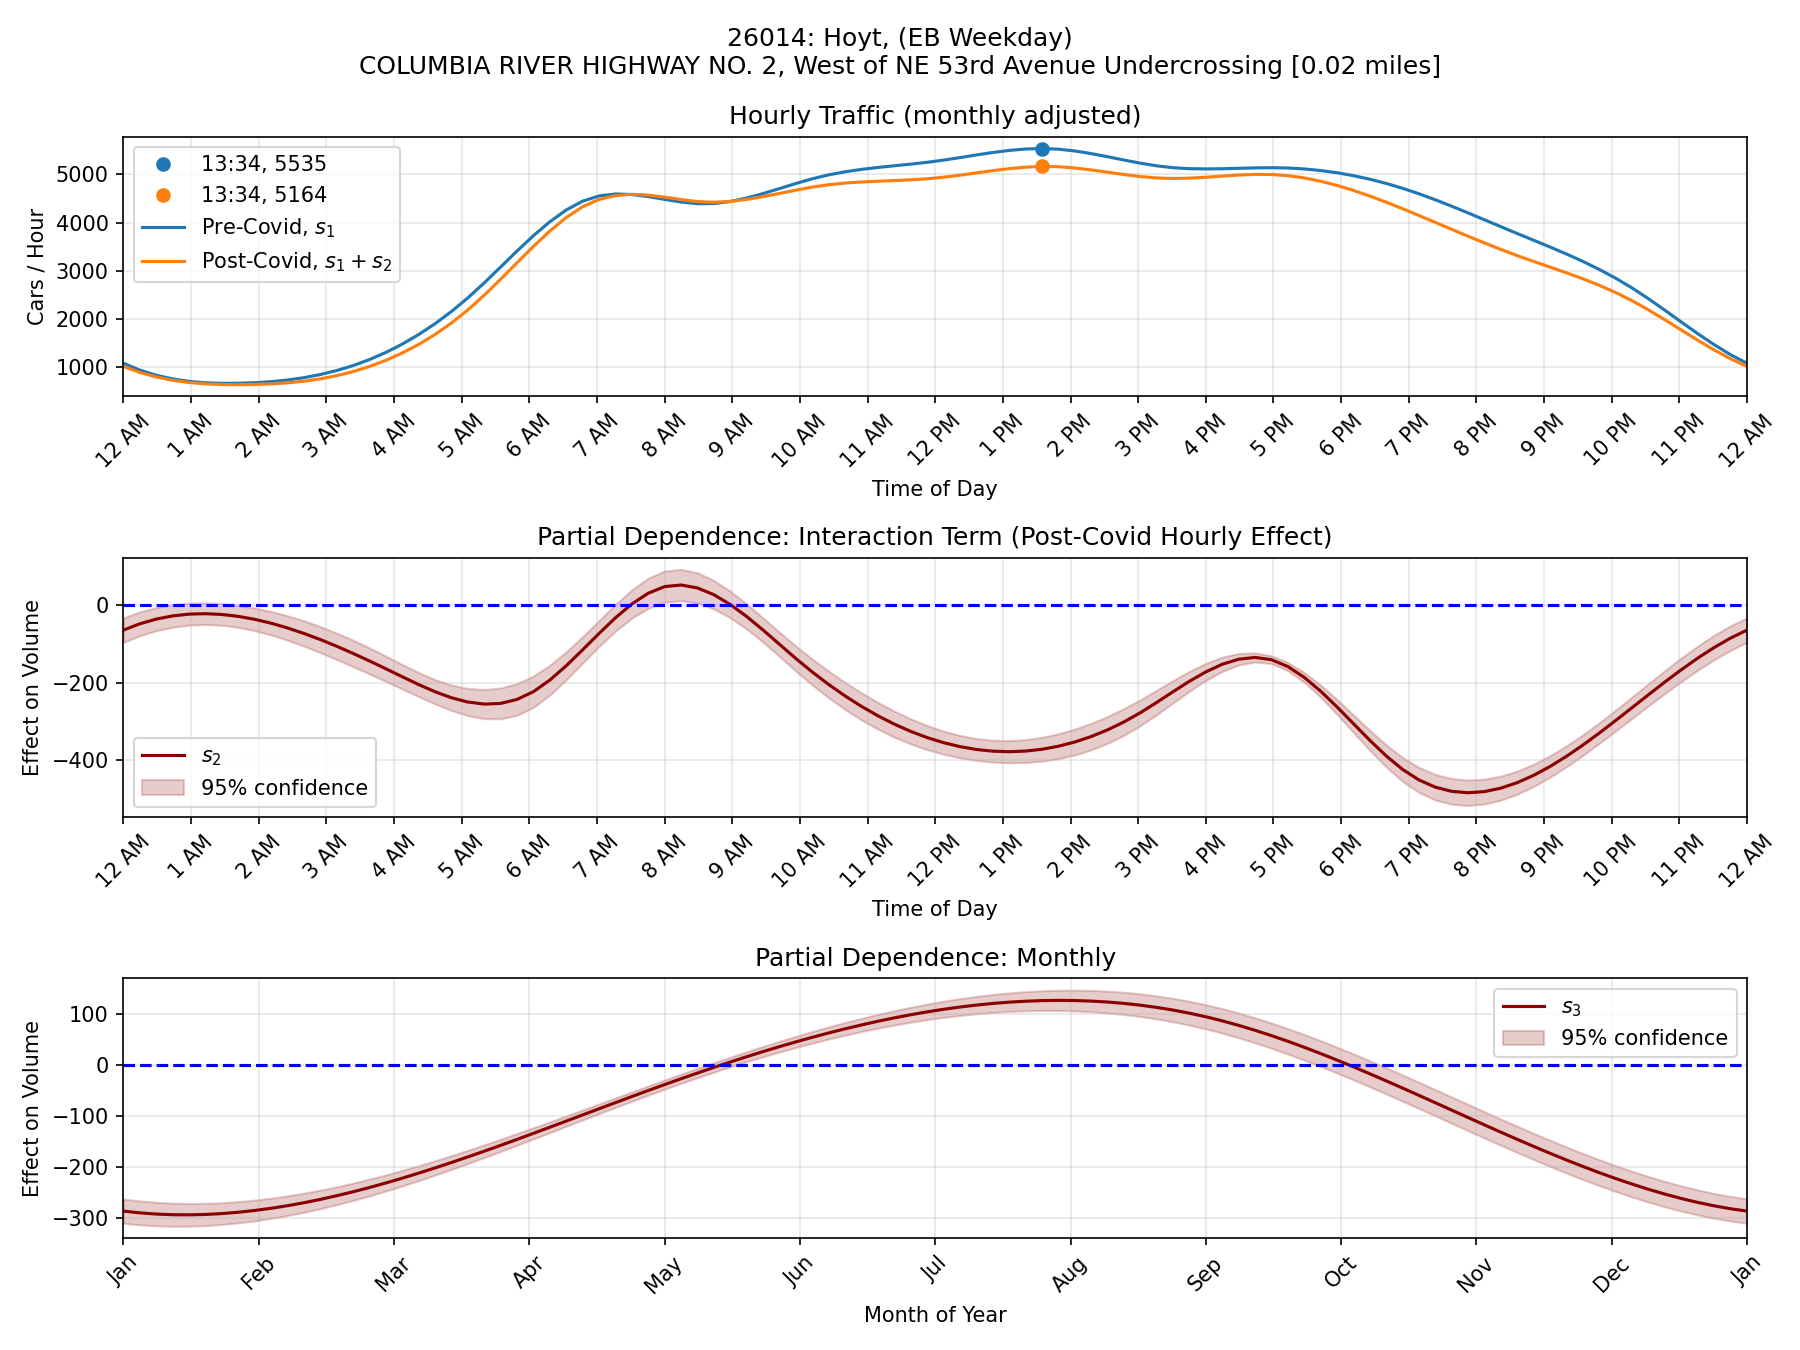
\includegraphics[width=\textwidth]{26014_Hoyt_EB_Weekday_gam.png}
	\end{subfigure}
	\hfill
	\begin{subfigure}[b]{0.45\textwidth}
		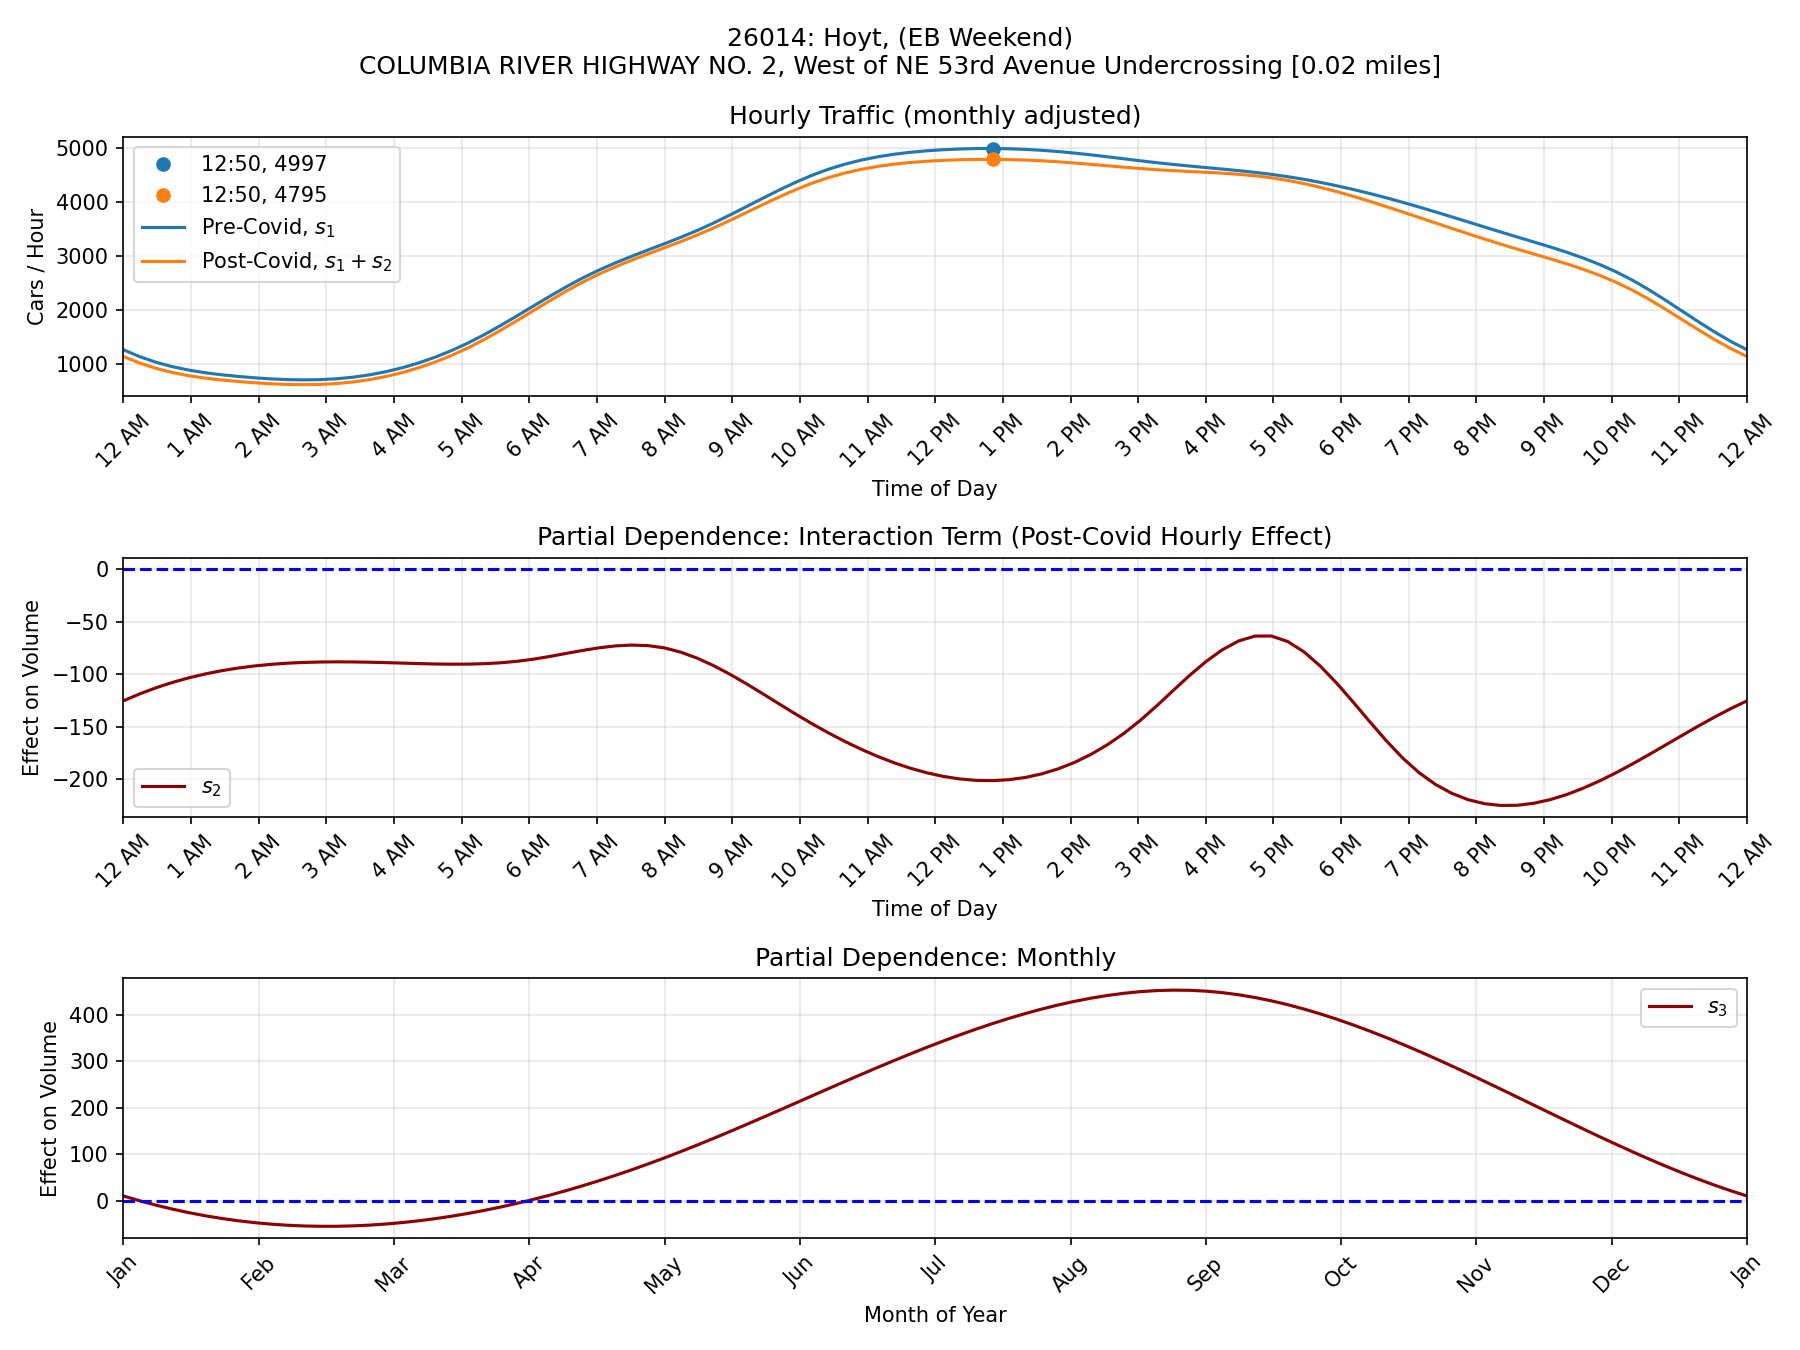
\includegraphics[width=\textwidth]{26014_Hoyt_EB_Weekend_gam.png}
	\end{subfigure}

	\begin{subfigure}[b]{0.45\textwidth}
		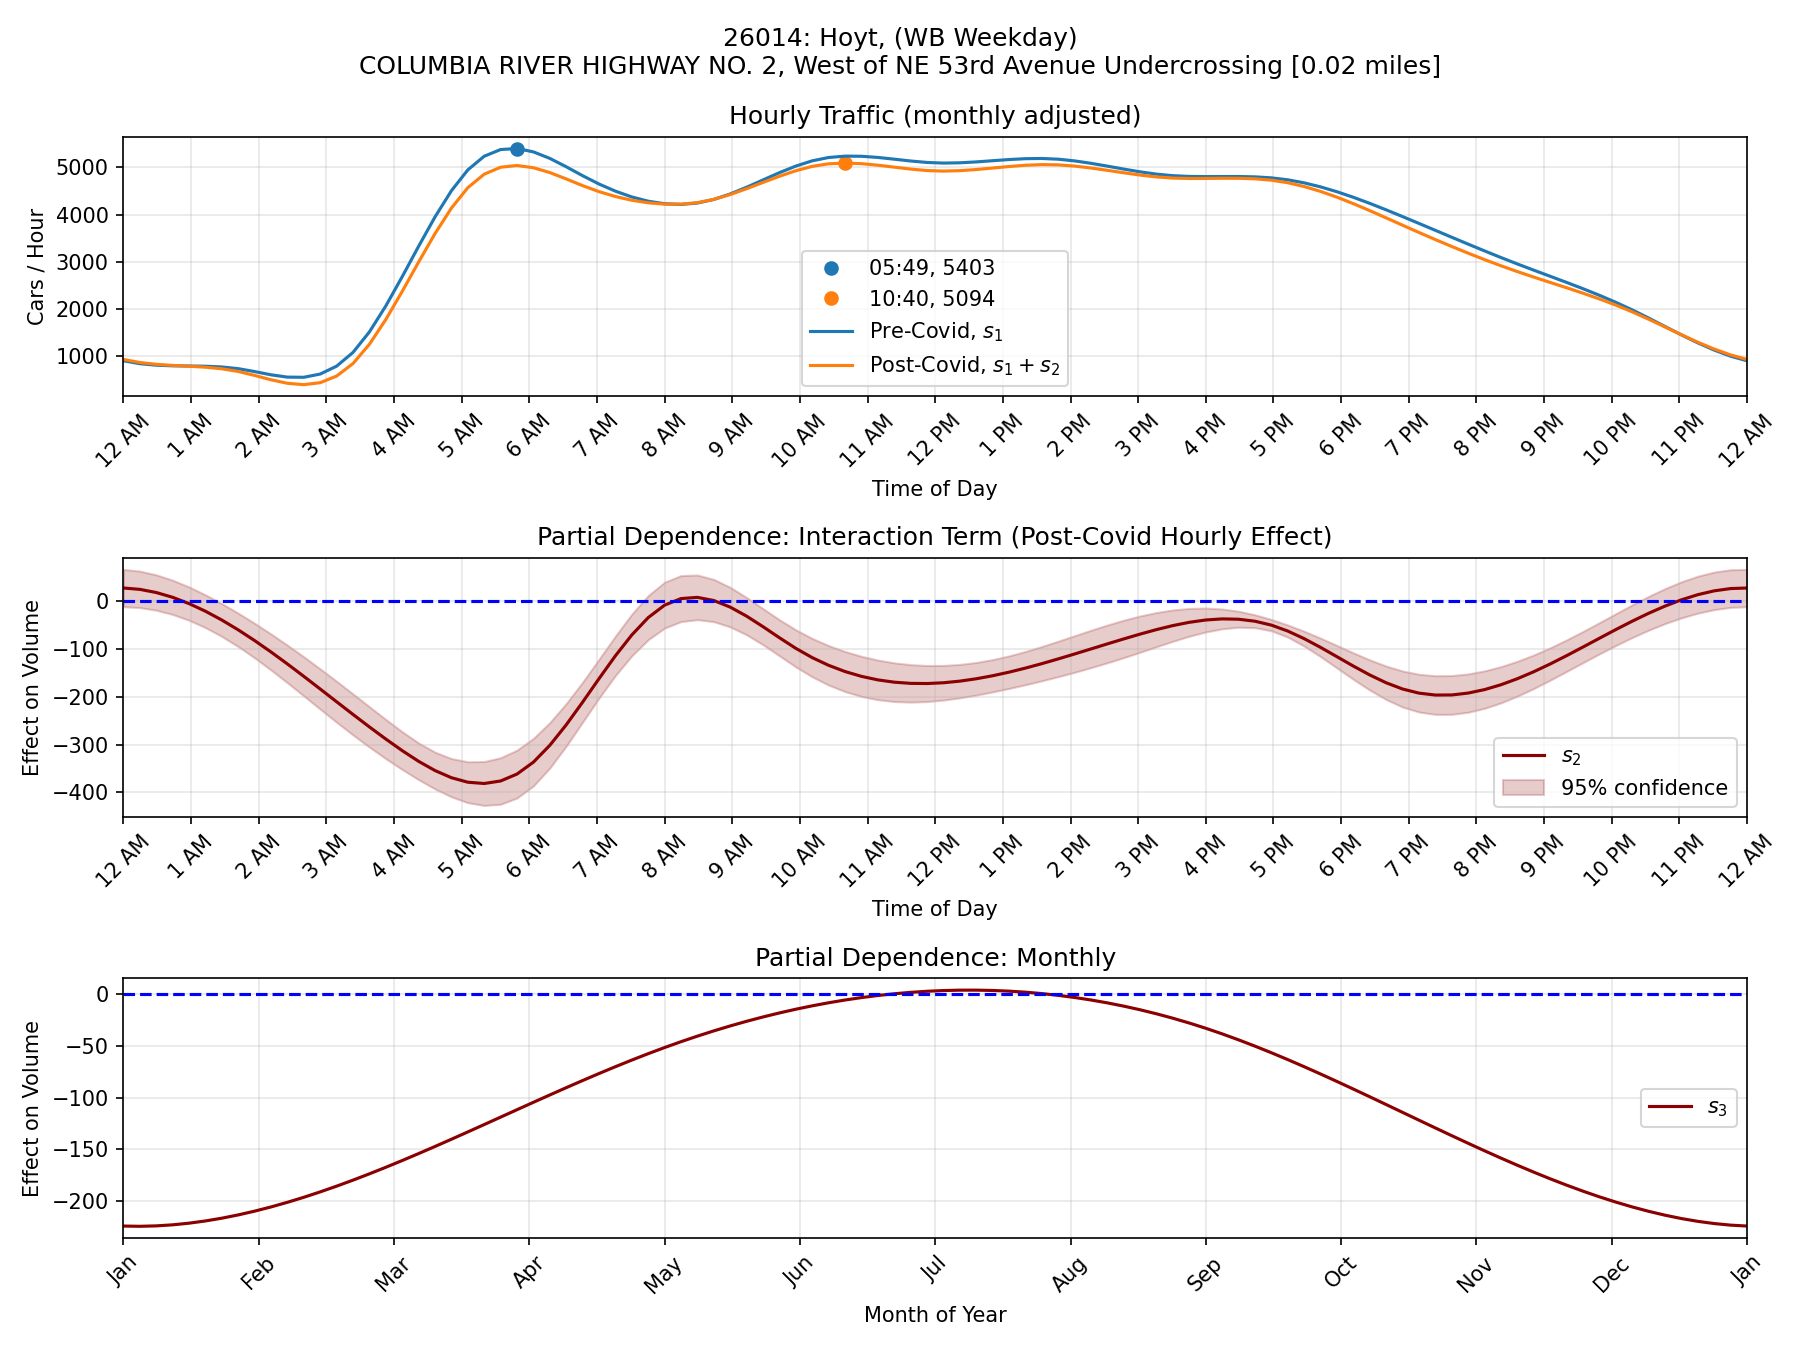
\includegraphics[width=\textwidth]{26014_Hoyt_WB_Weekday_gam.png}
	\end{subfigure}
	\hfill
	\begin{subfigure}[b]{0.45\textwidth}
		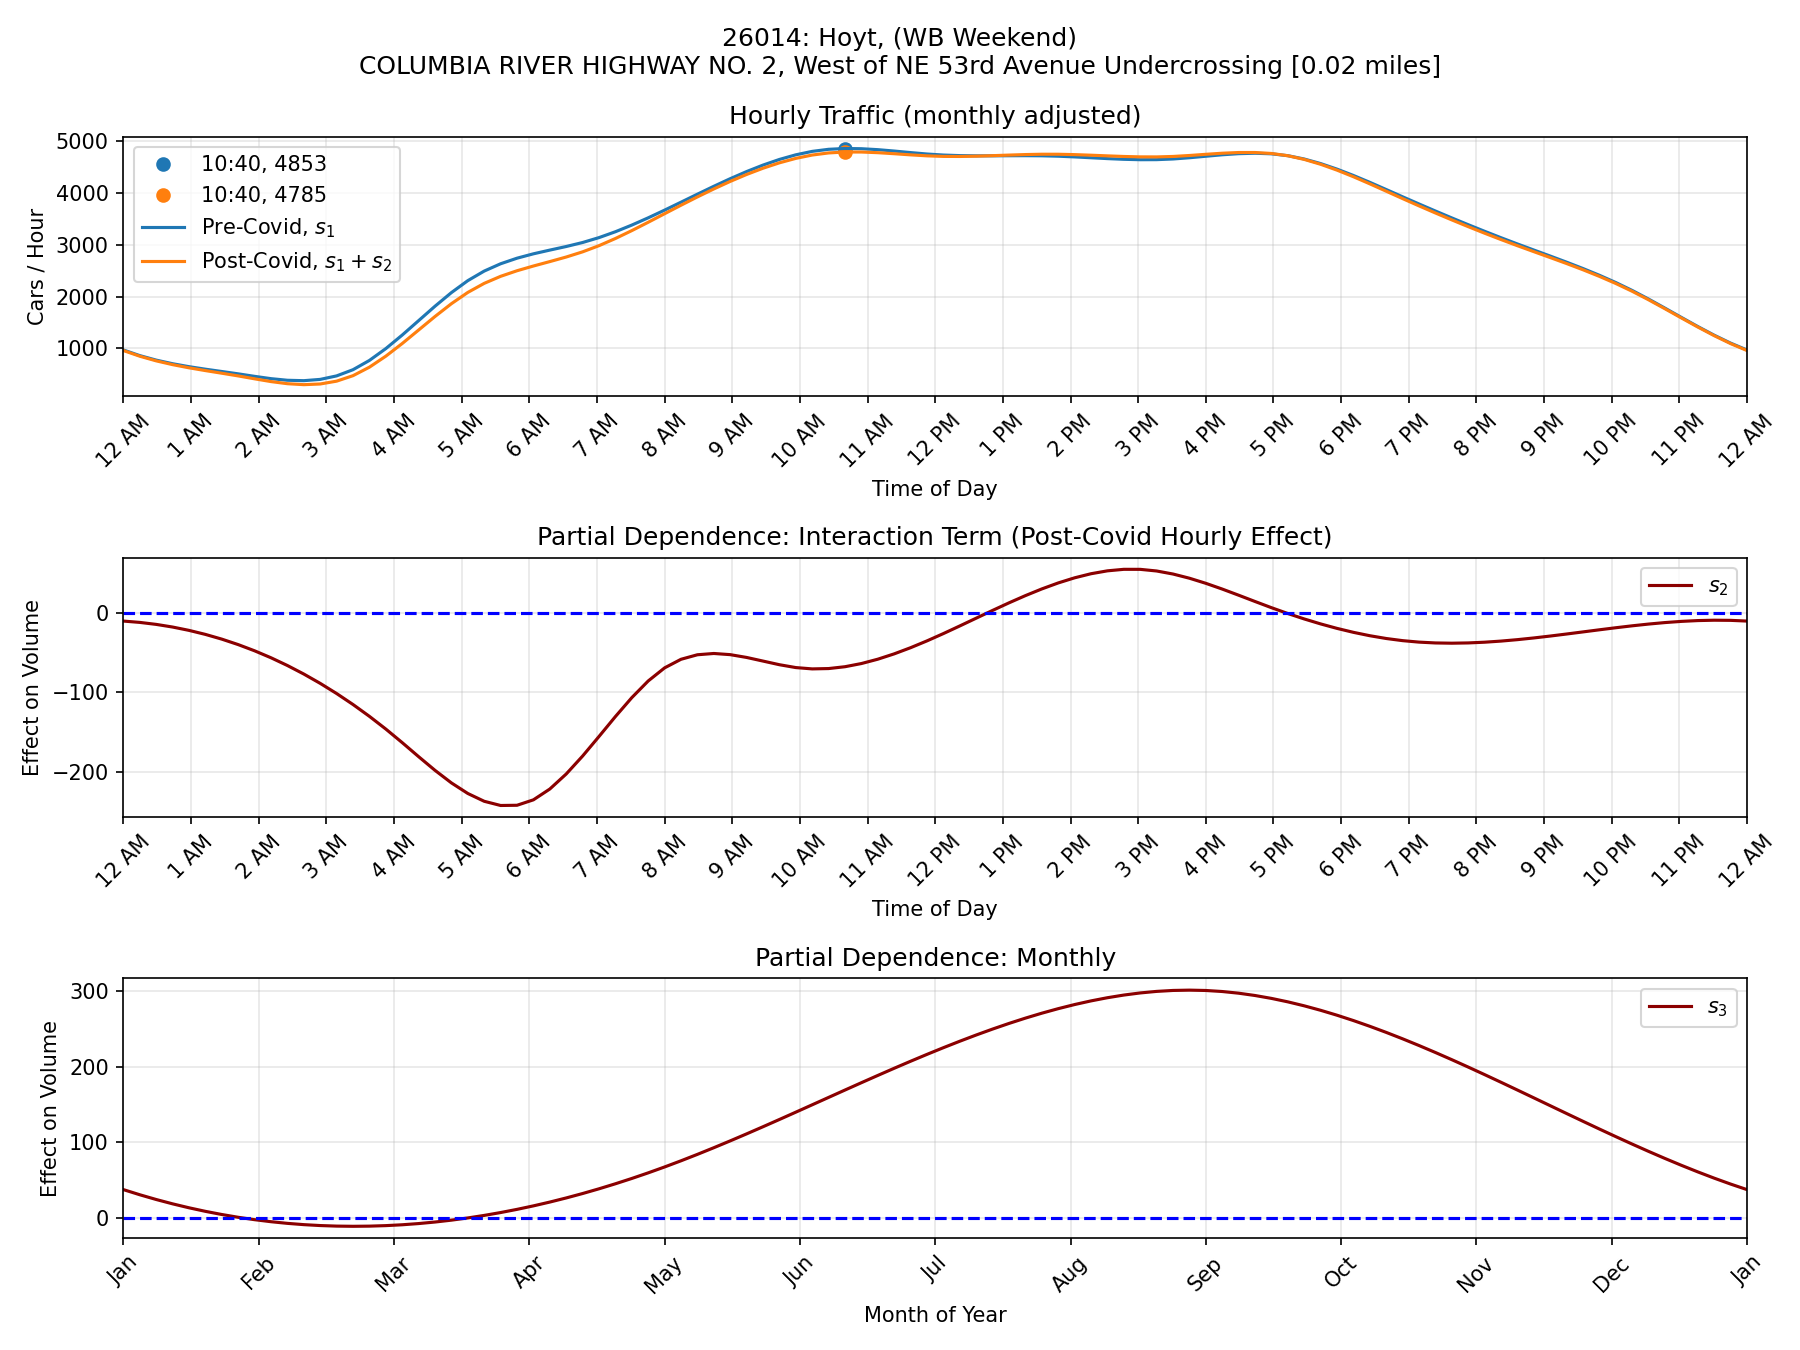
\includegraphics[width=\textwidth]{26014_Hoyt_WB_Weekend_gam.png}
	\end{subfigure}
\end{figure}

\begin{figure}[H]
	\centering
	\begin{subfigure}[b]{0.45\textwidth}
		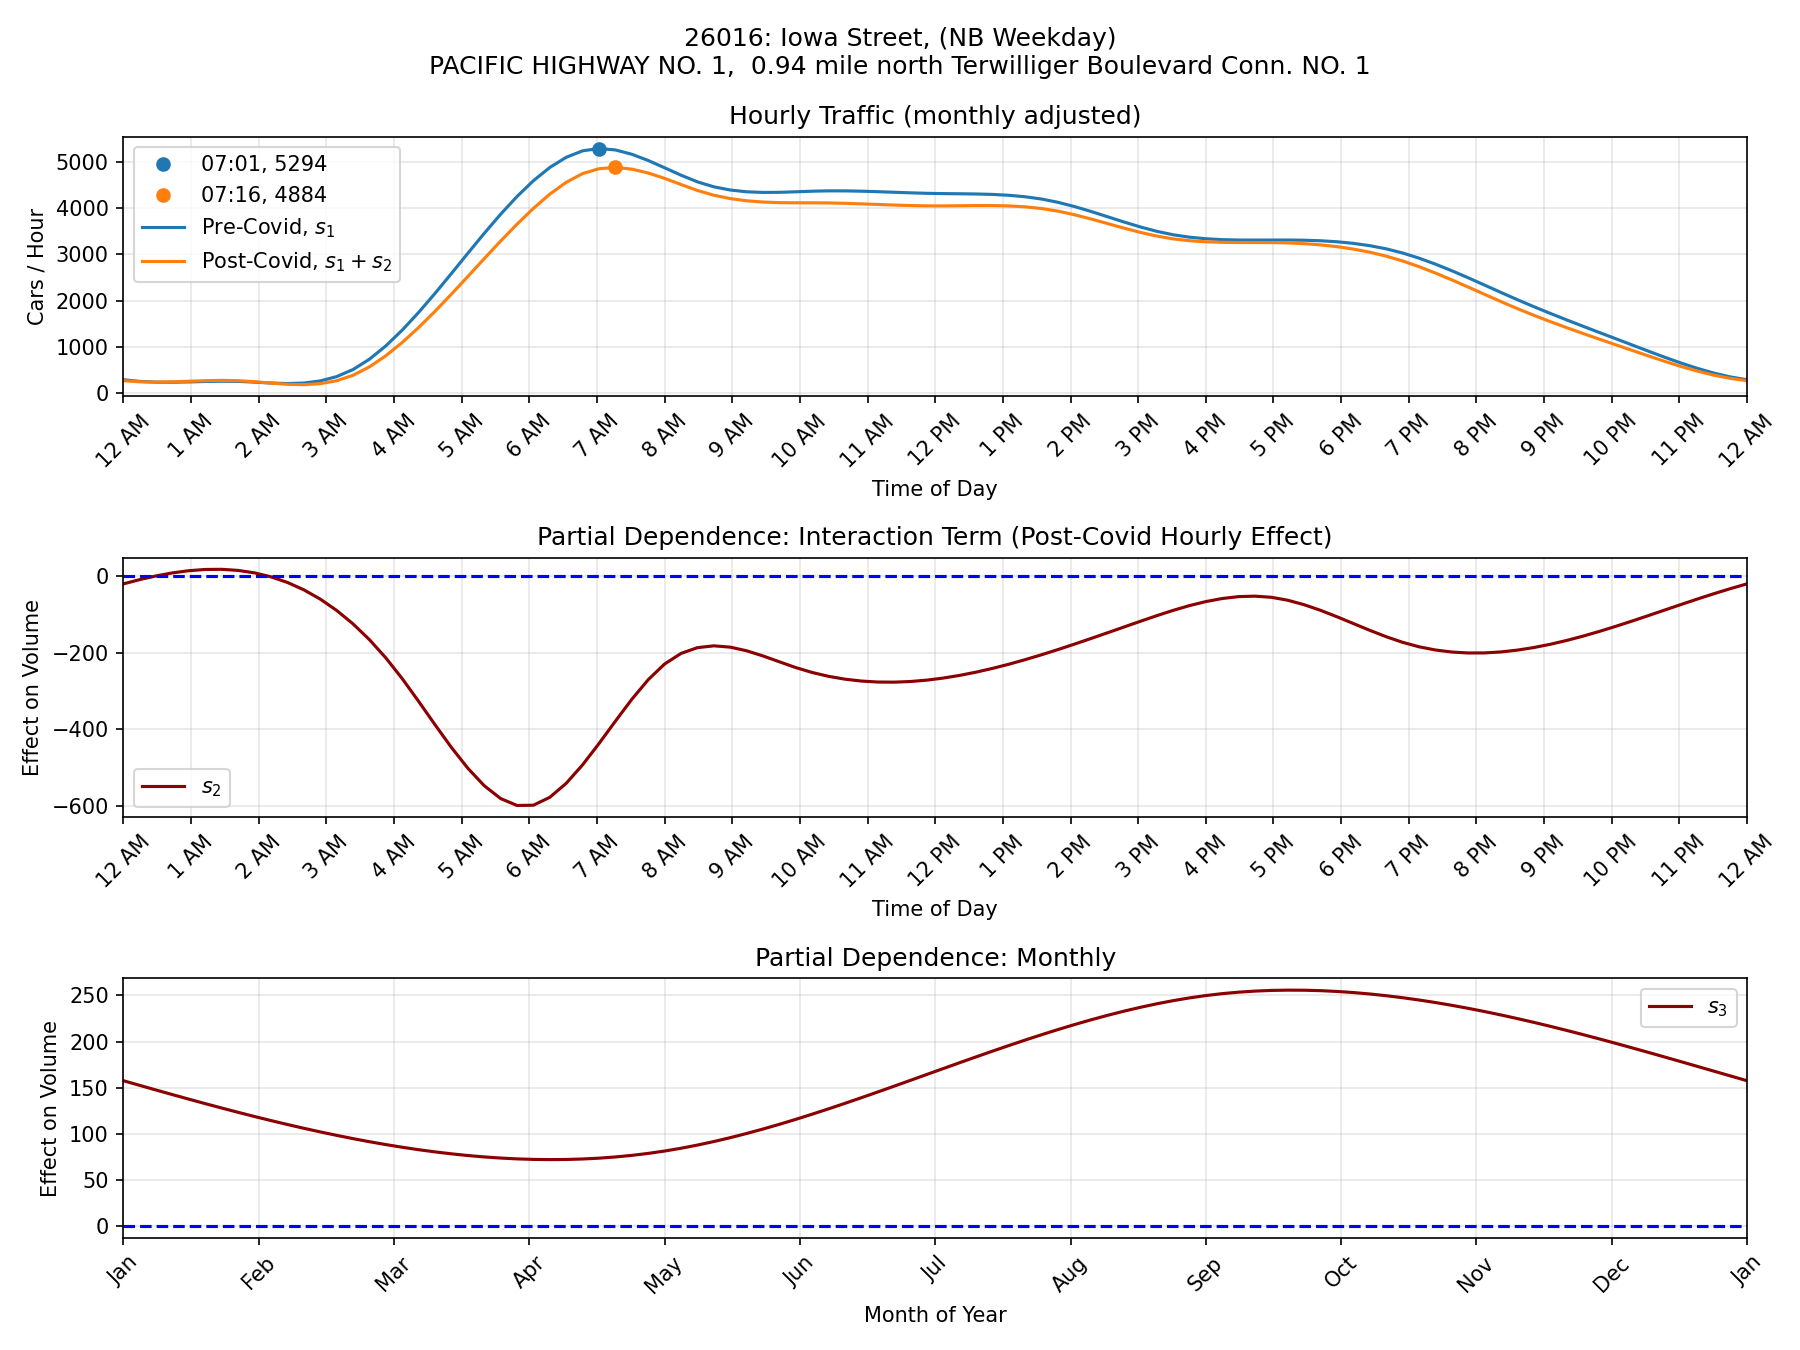
\includegraphics[width=\textwidth]{26016_Iowa-Street_NB_Weekday_gam.png}
	\end{subfigure}
	\hfill
	\begin{subfigure}[b]{0.45\textwidth}
		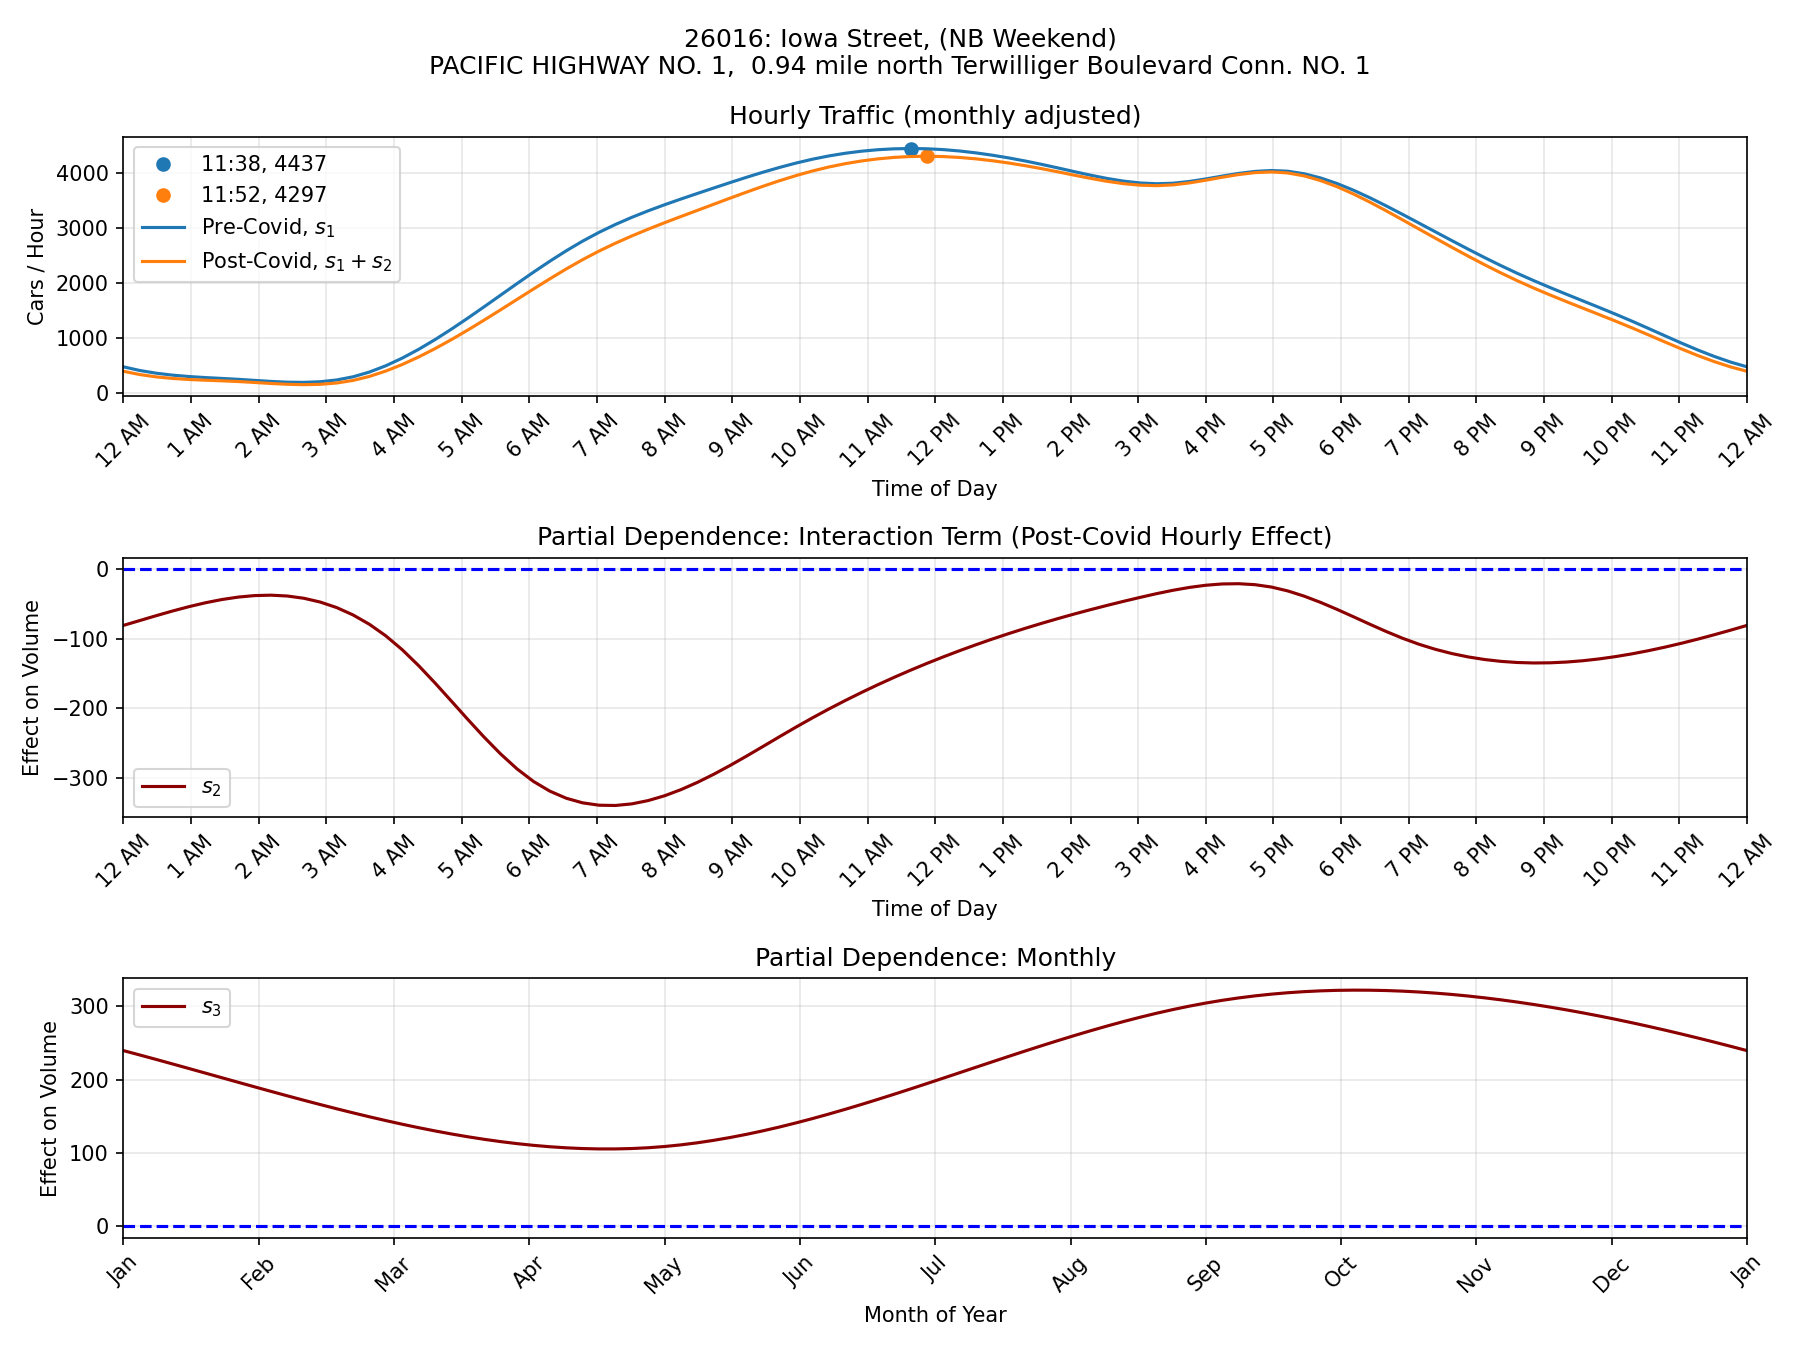
\includegraphics[width=\textwidth]{26016_Iowa-Street_NB_Weekend_gam.png}
	\end{subfigure}

	\begin{subfigure}[b]{0.45\textwidth}
		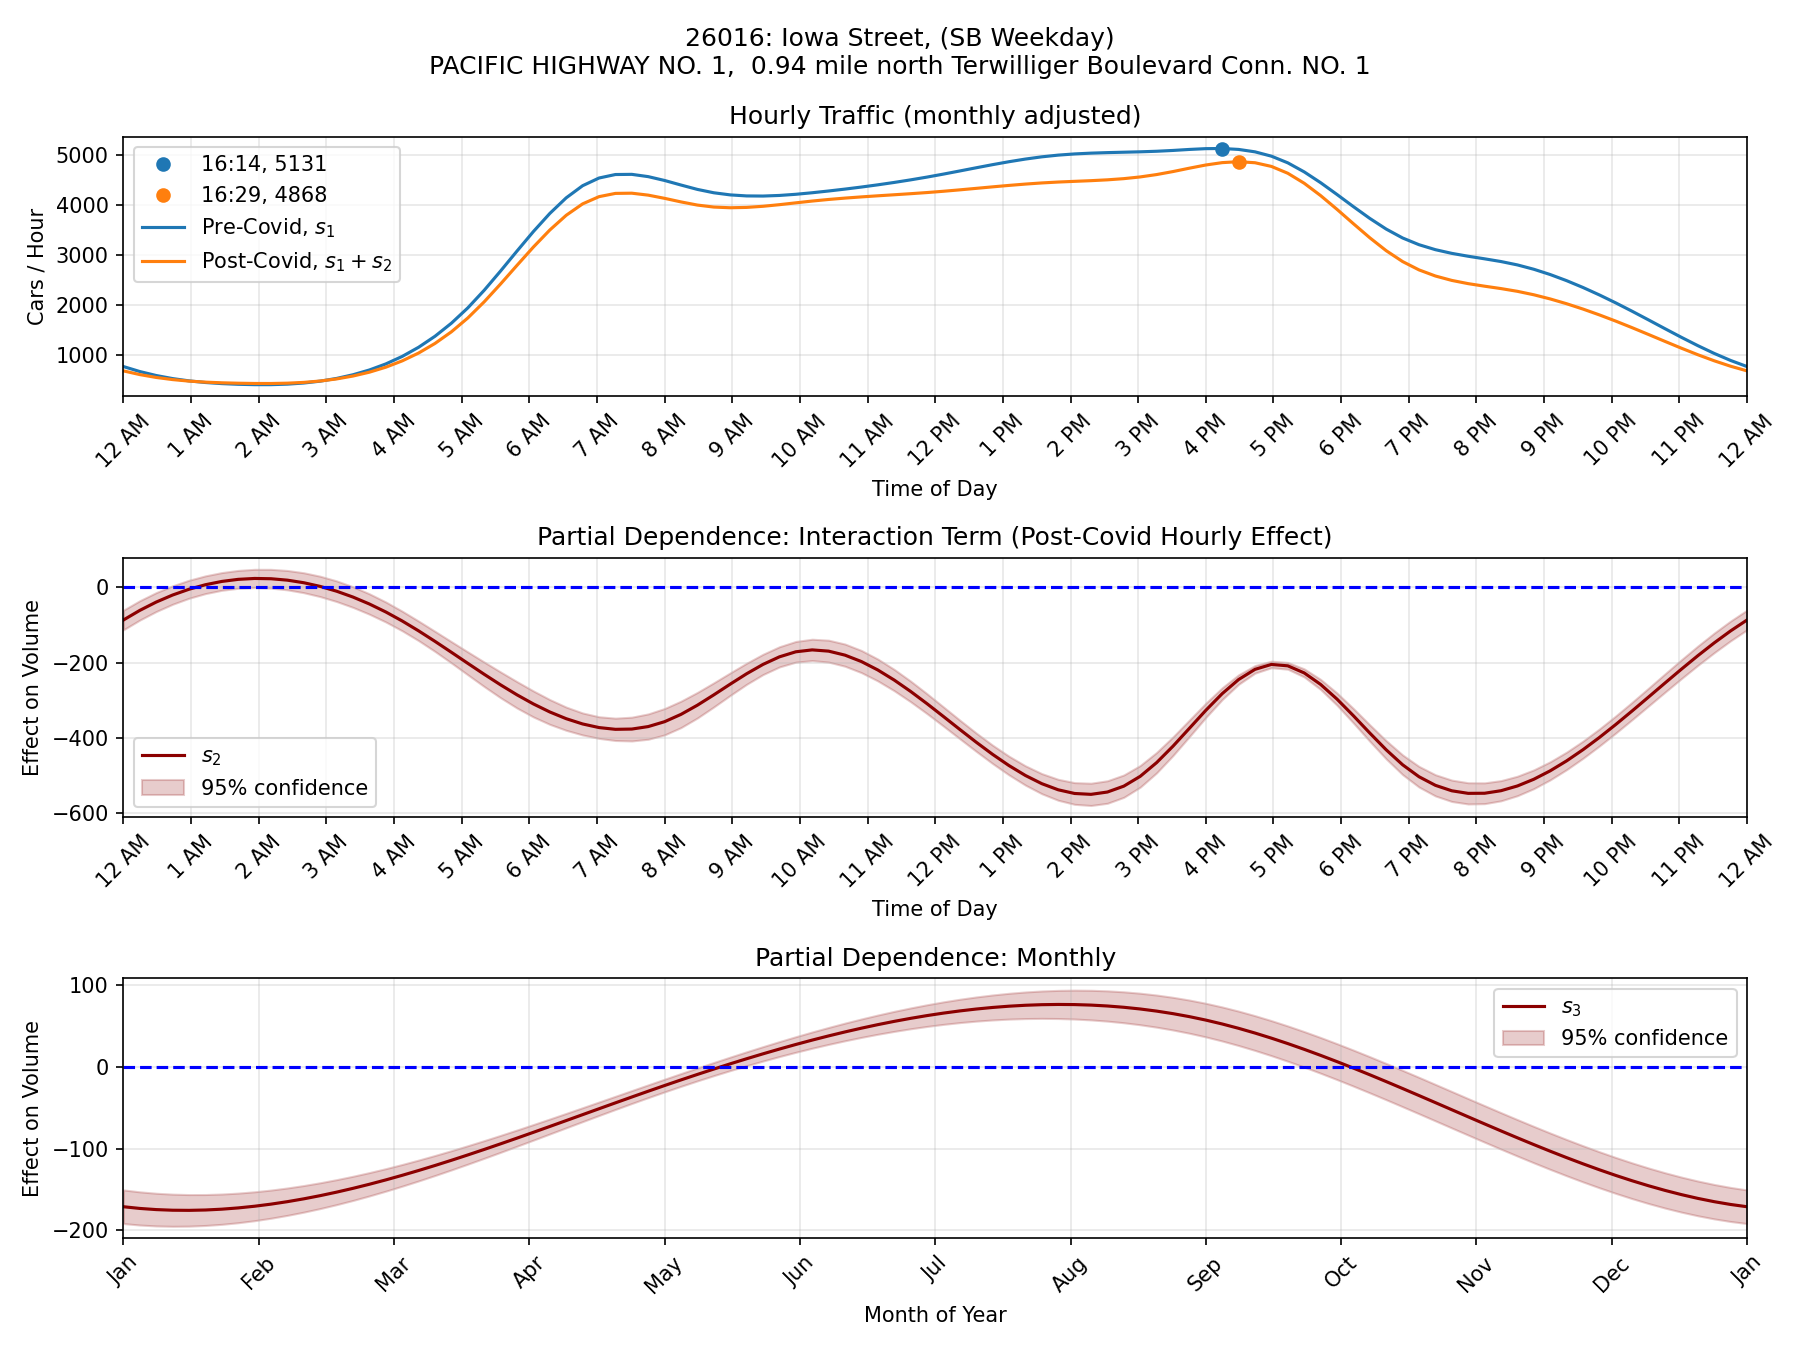
\includegraphics[width=\textwidth]{26016_Iowa-Street_SB_Weekday_gam.png}
	\end{subfigure}
	\hfill
	\begin{subfigure}[b]{0.45\textwidth}
		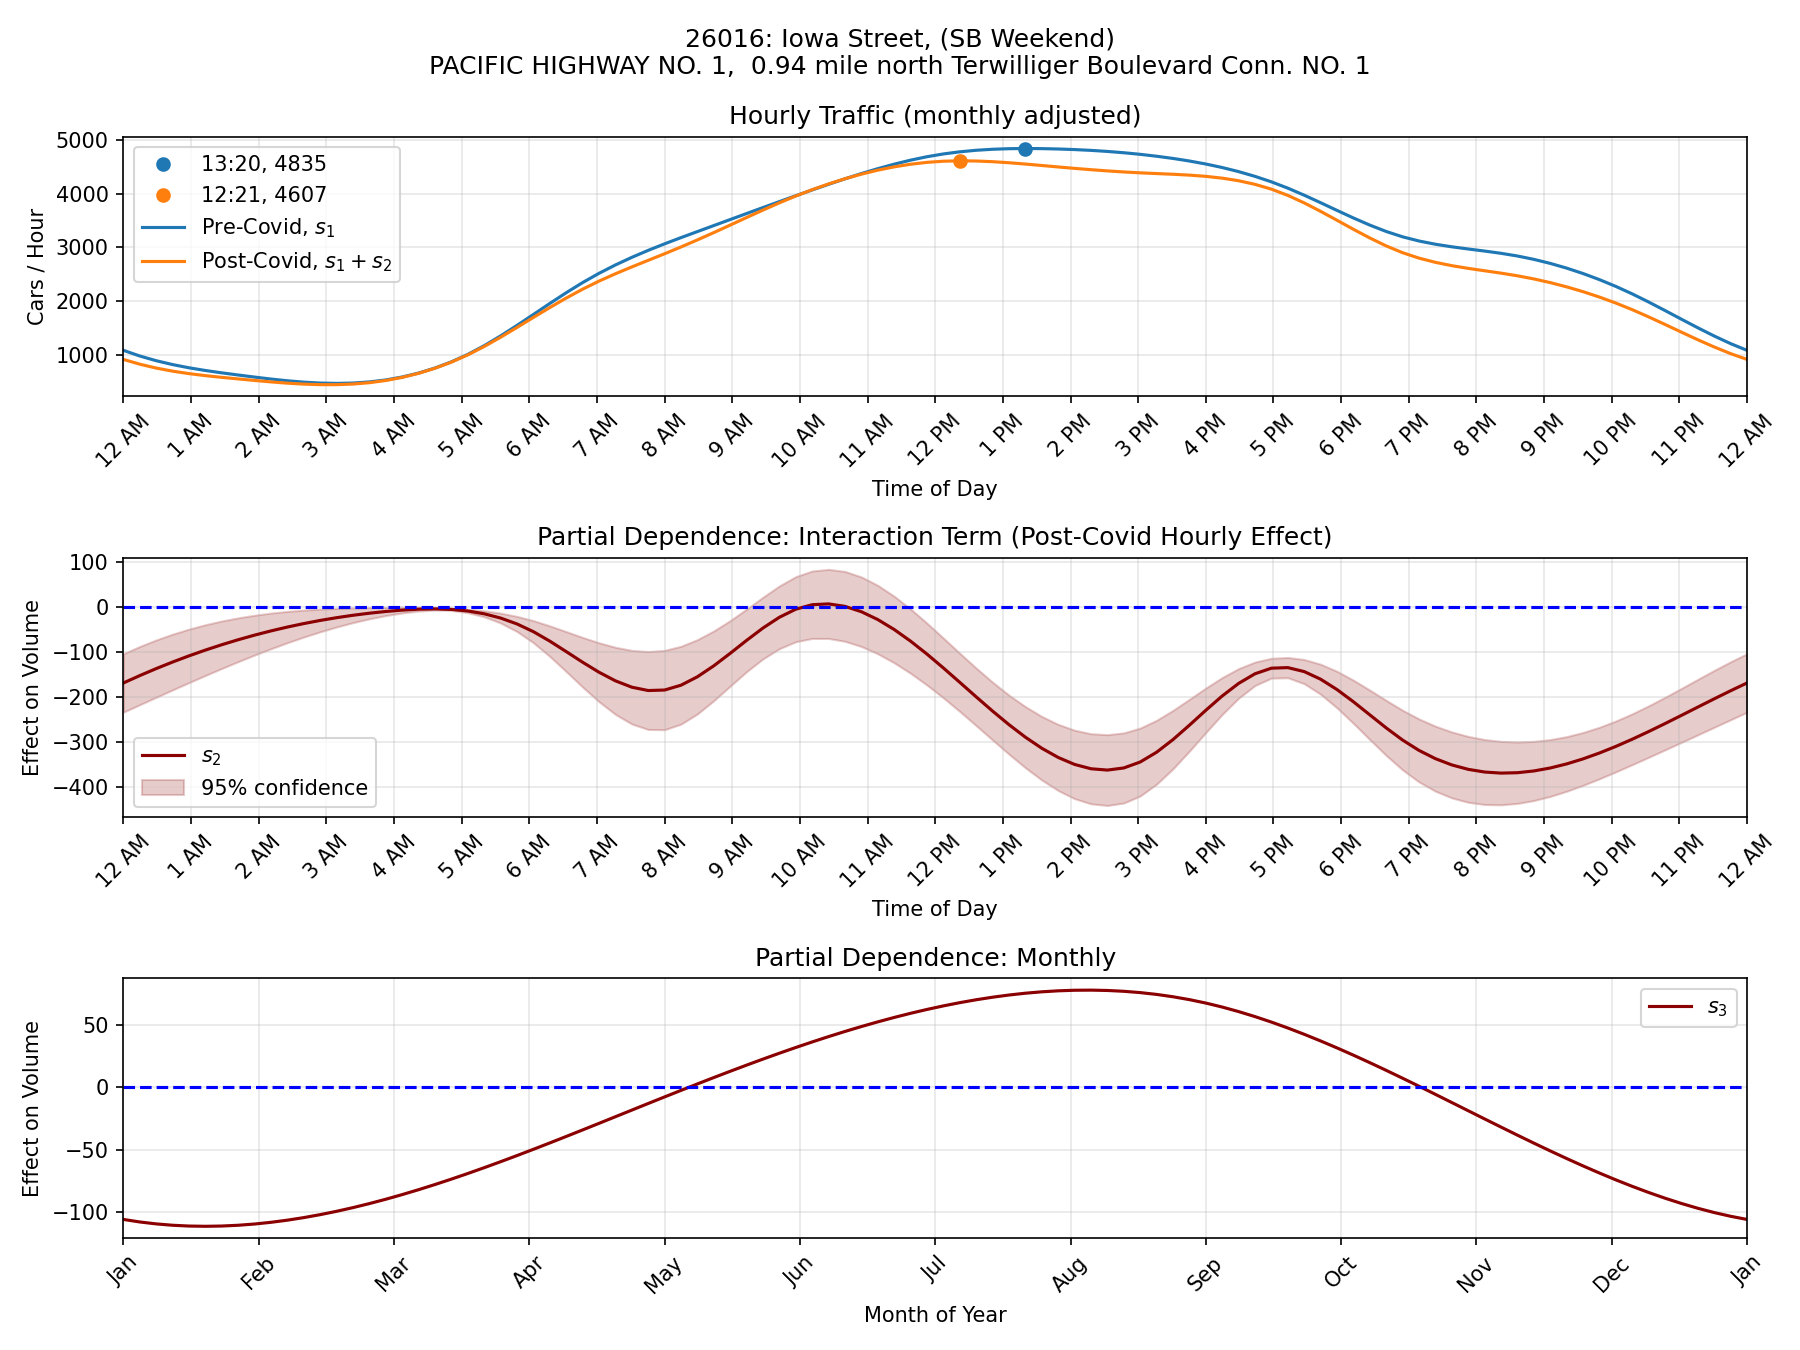
\includegraphics[width=\textwidth]{26016_Iowa-Street_SB_Weekend_gam.png}
	\end{subfigure}
\end{figure}

\begin{figure}[H]
	\centering
	\begin{subfigure}[b]{0.45\textwidth}
		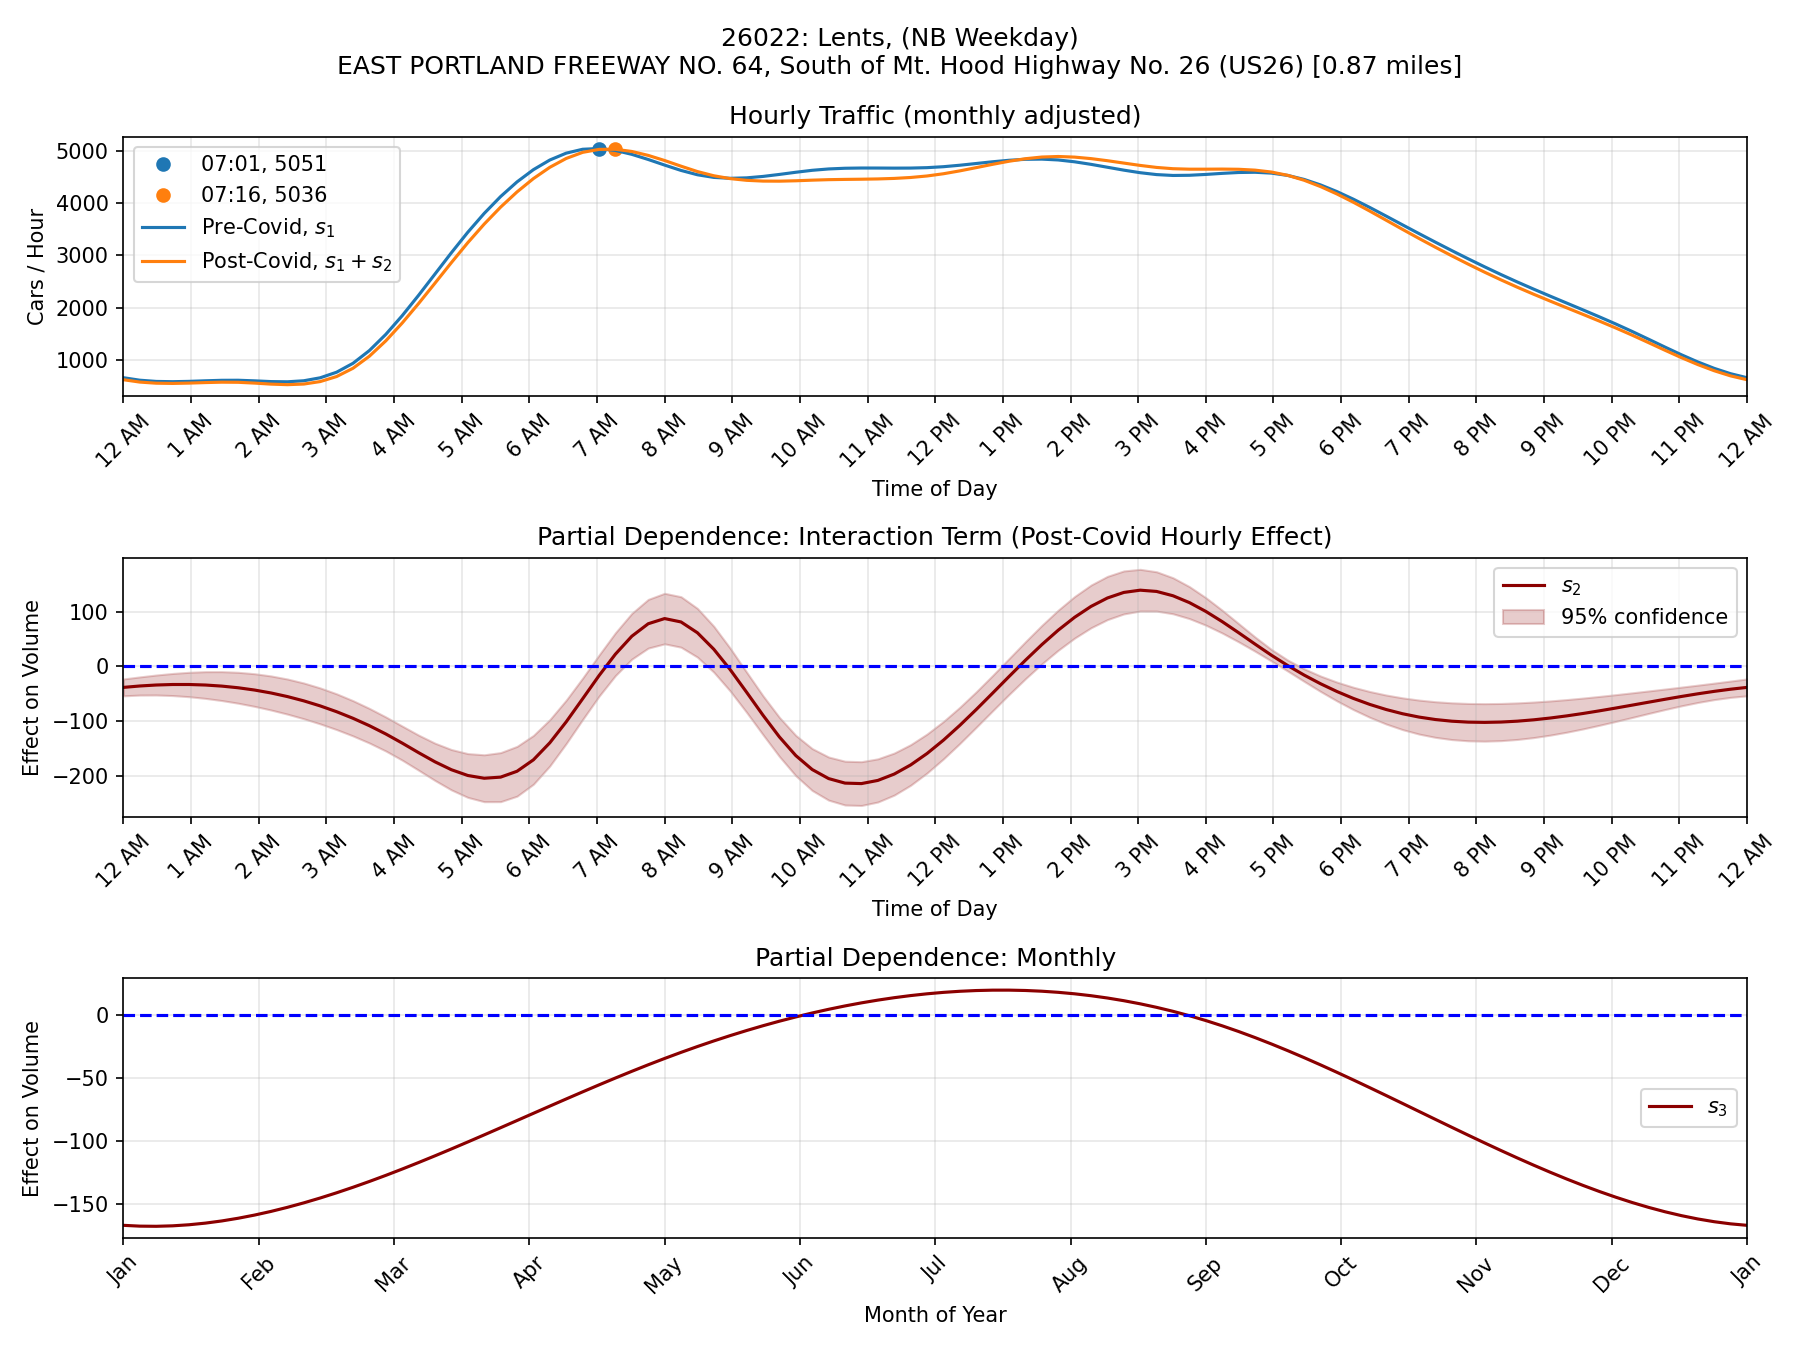
\includegraphics[width=\textwidth]{26022_Lents_NB_Weekday_gam.png}
	\end{subfigure}
	\hfill
	\begin{subfigure}[b]{0.45\textwidth}
		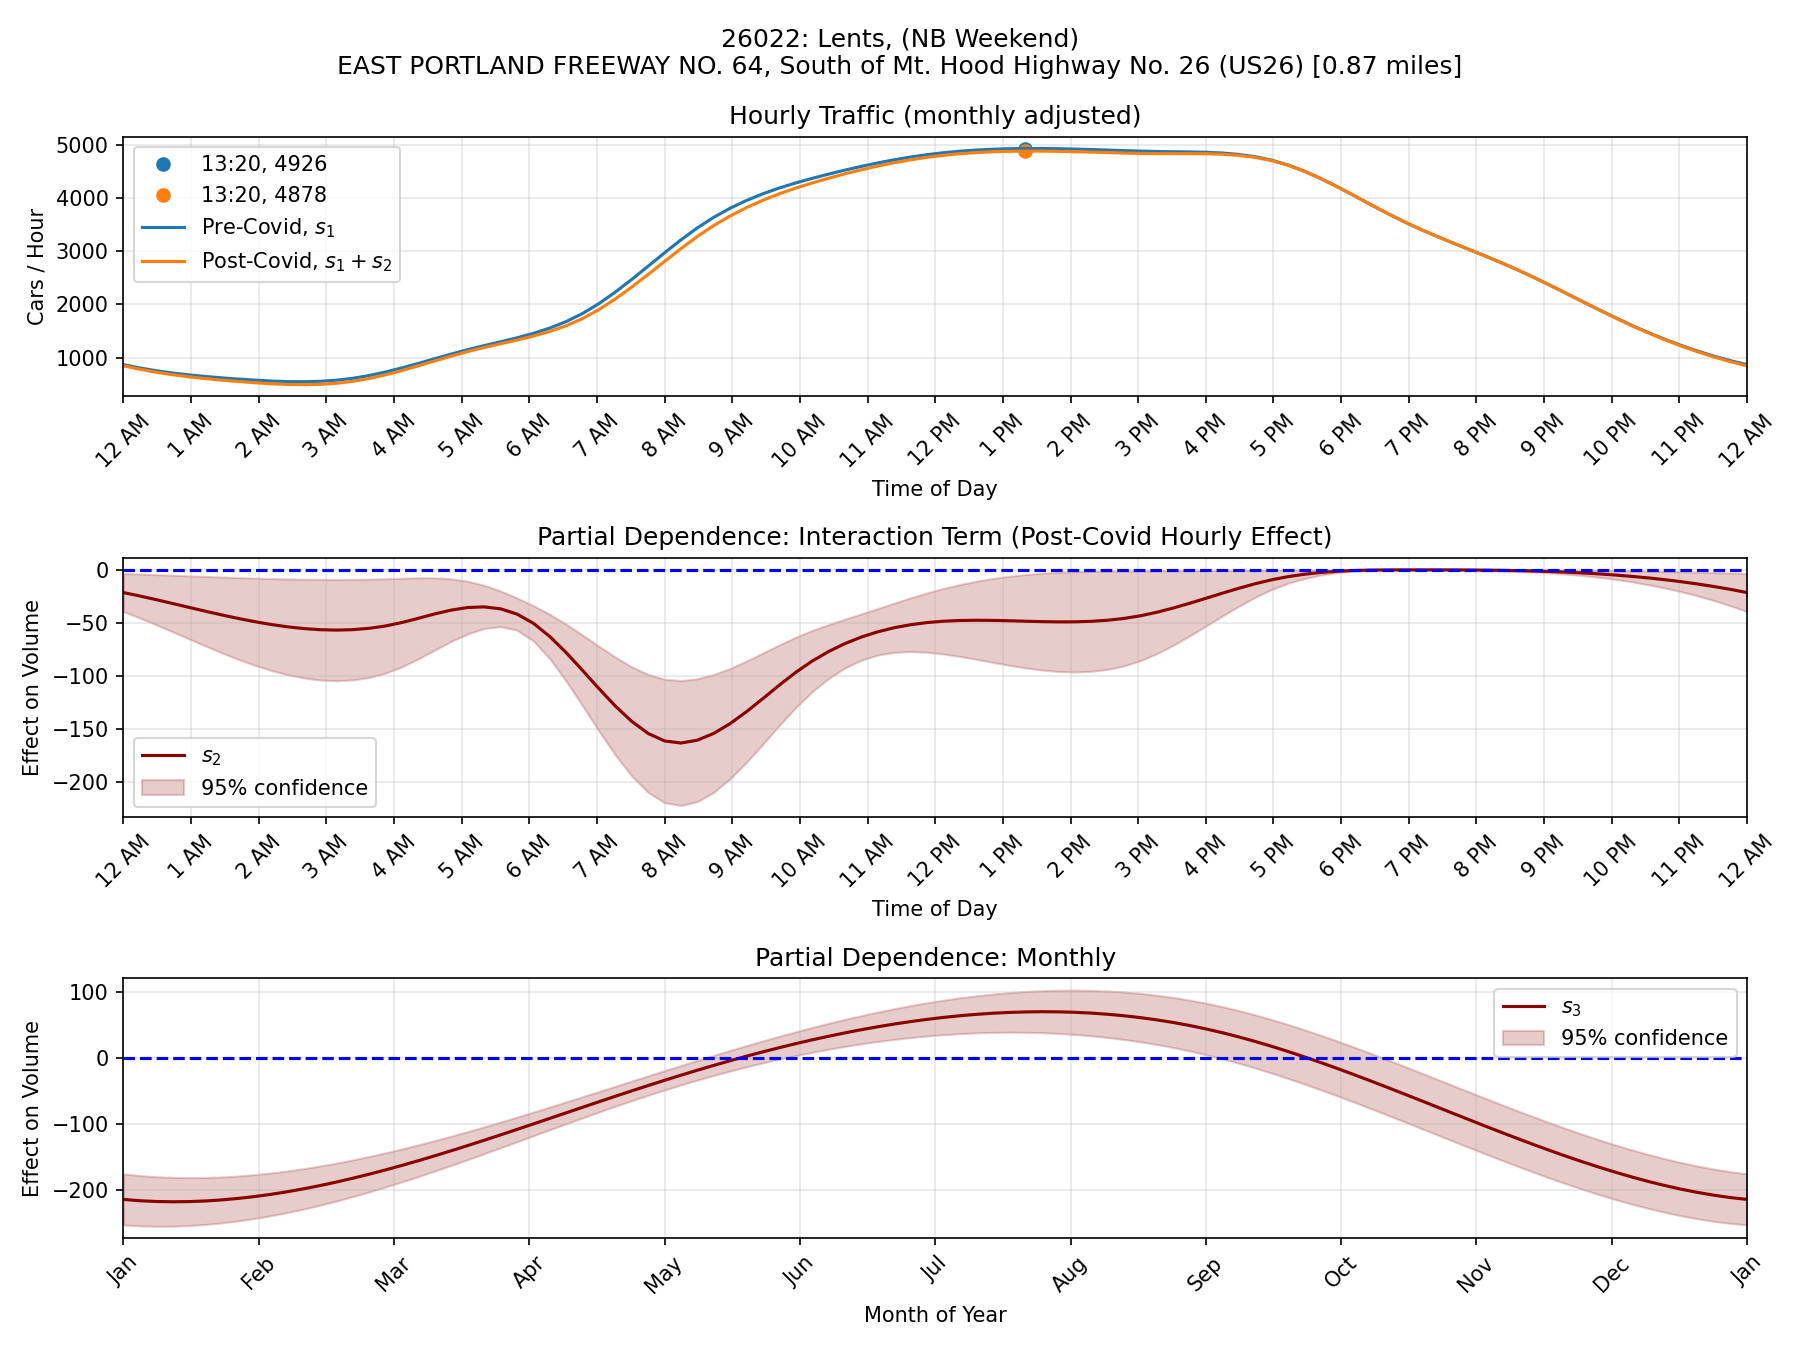
\includegraphics[width=\textwidth]{26022_Lents_NB_Weekend_gam.png}
	\end{subfigure}

	\begin{subfigure}[b]{0.45\textwidth}
		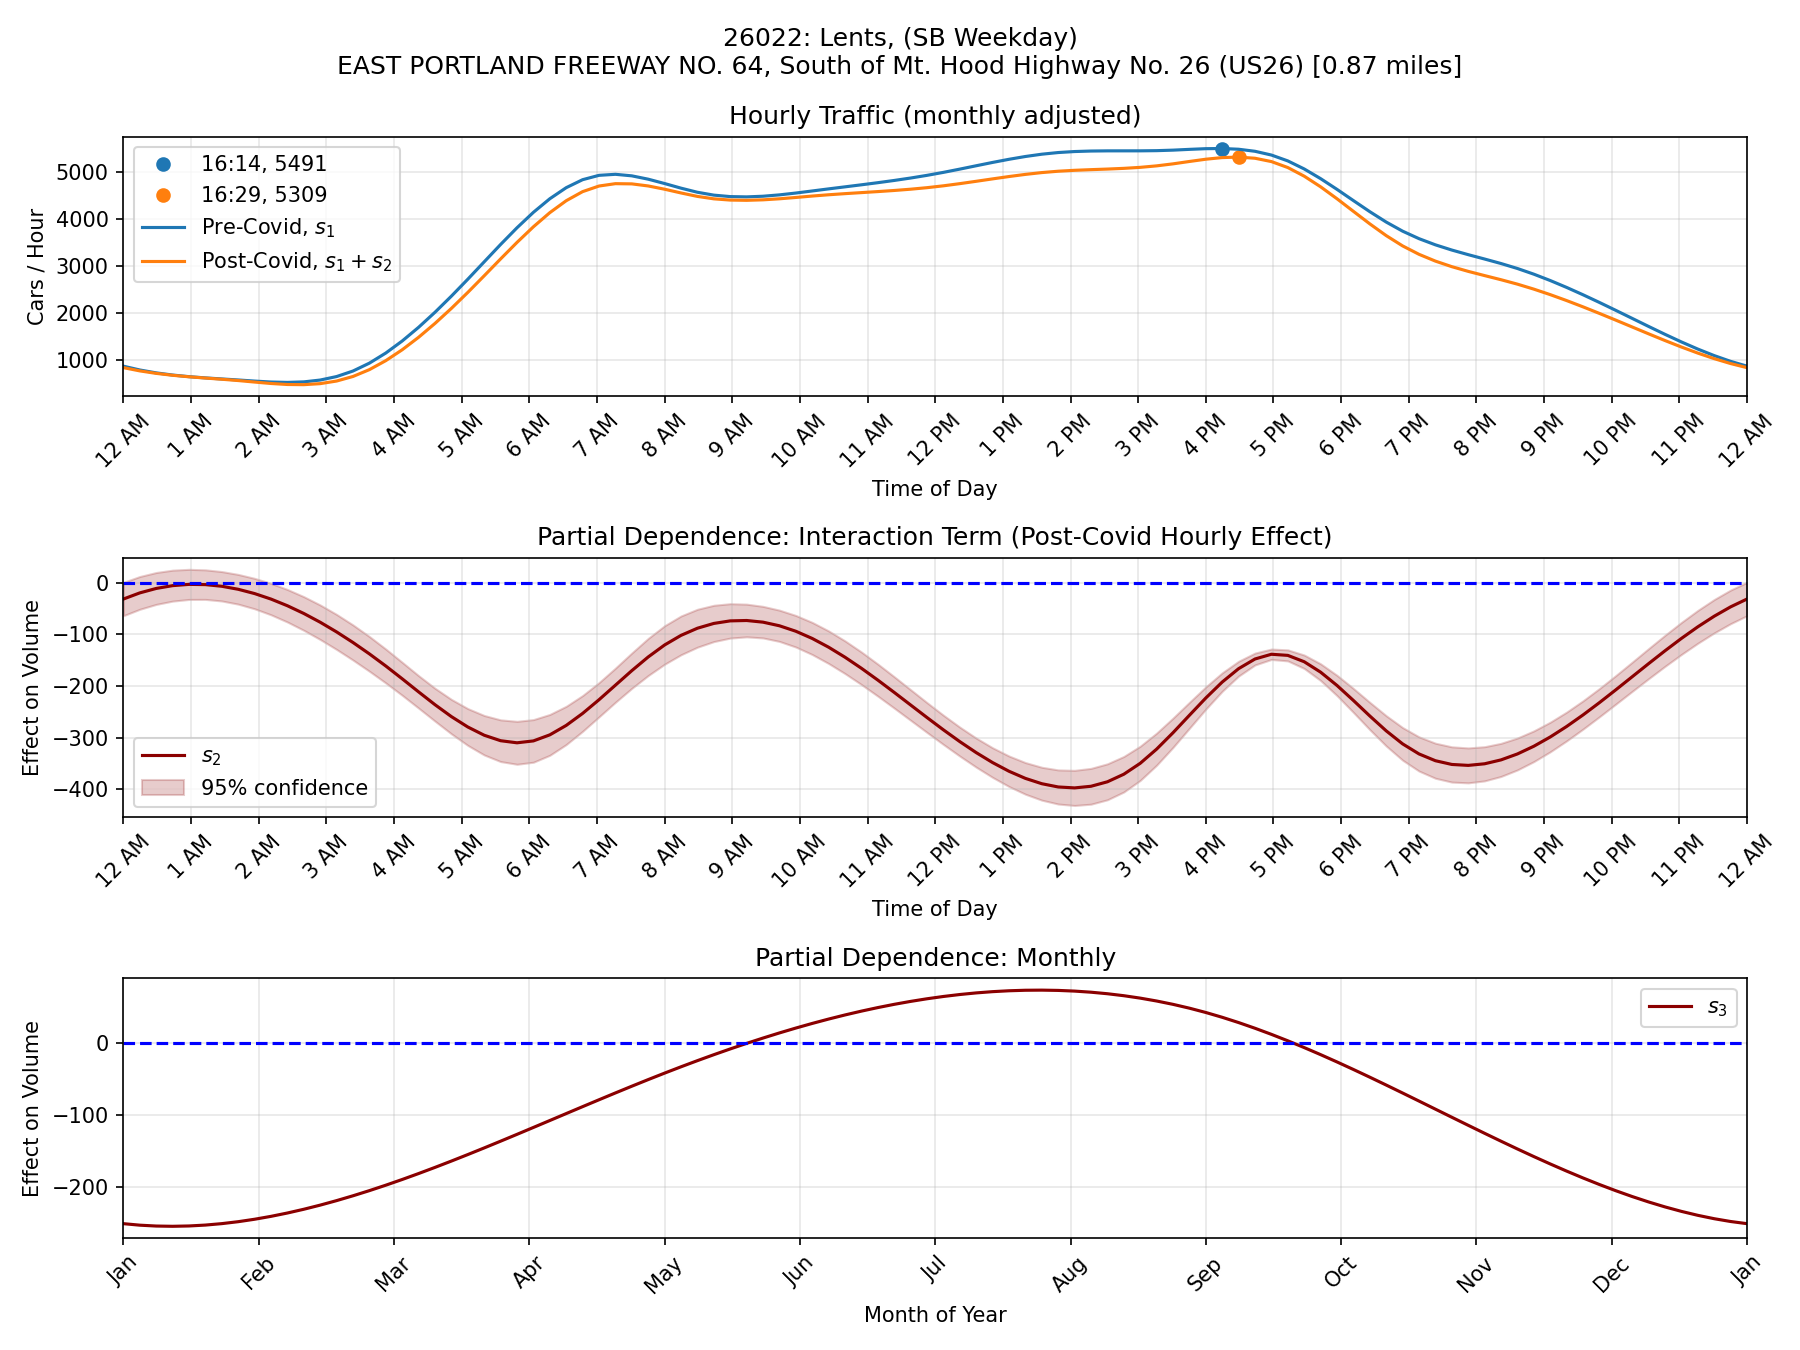
\includegraphics[width=\textwidth]{26022_Lents_SB_Weekday_gam.png}
	\end{subfigure}
	\hfill
	\begin{subfigure}[b]{0.45\textwidth}
		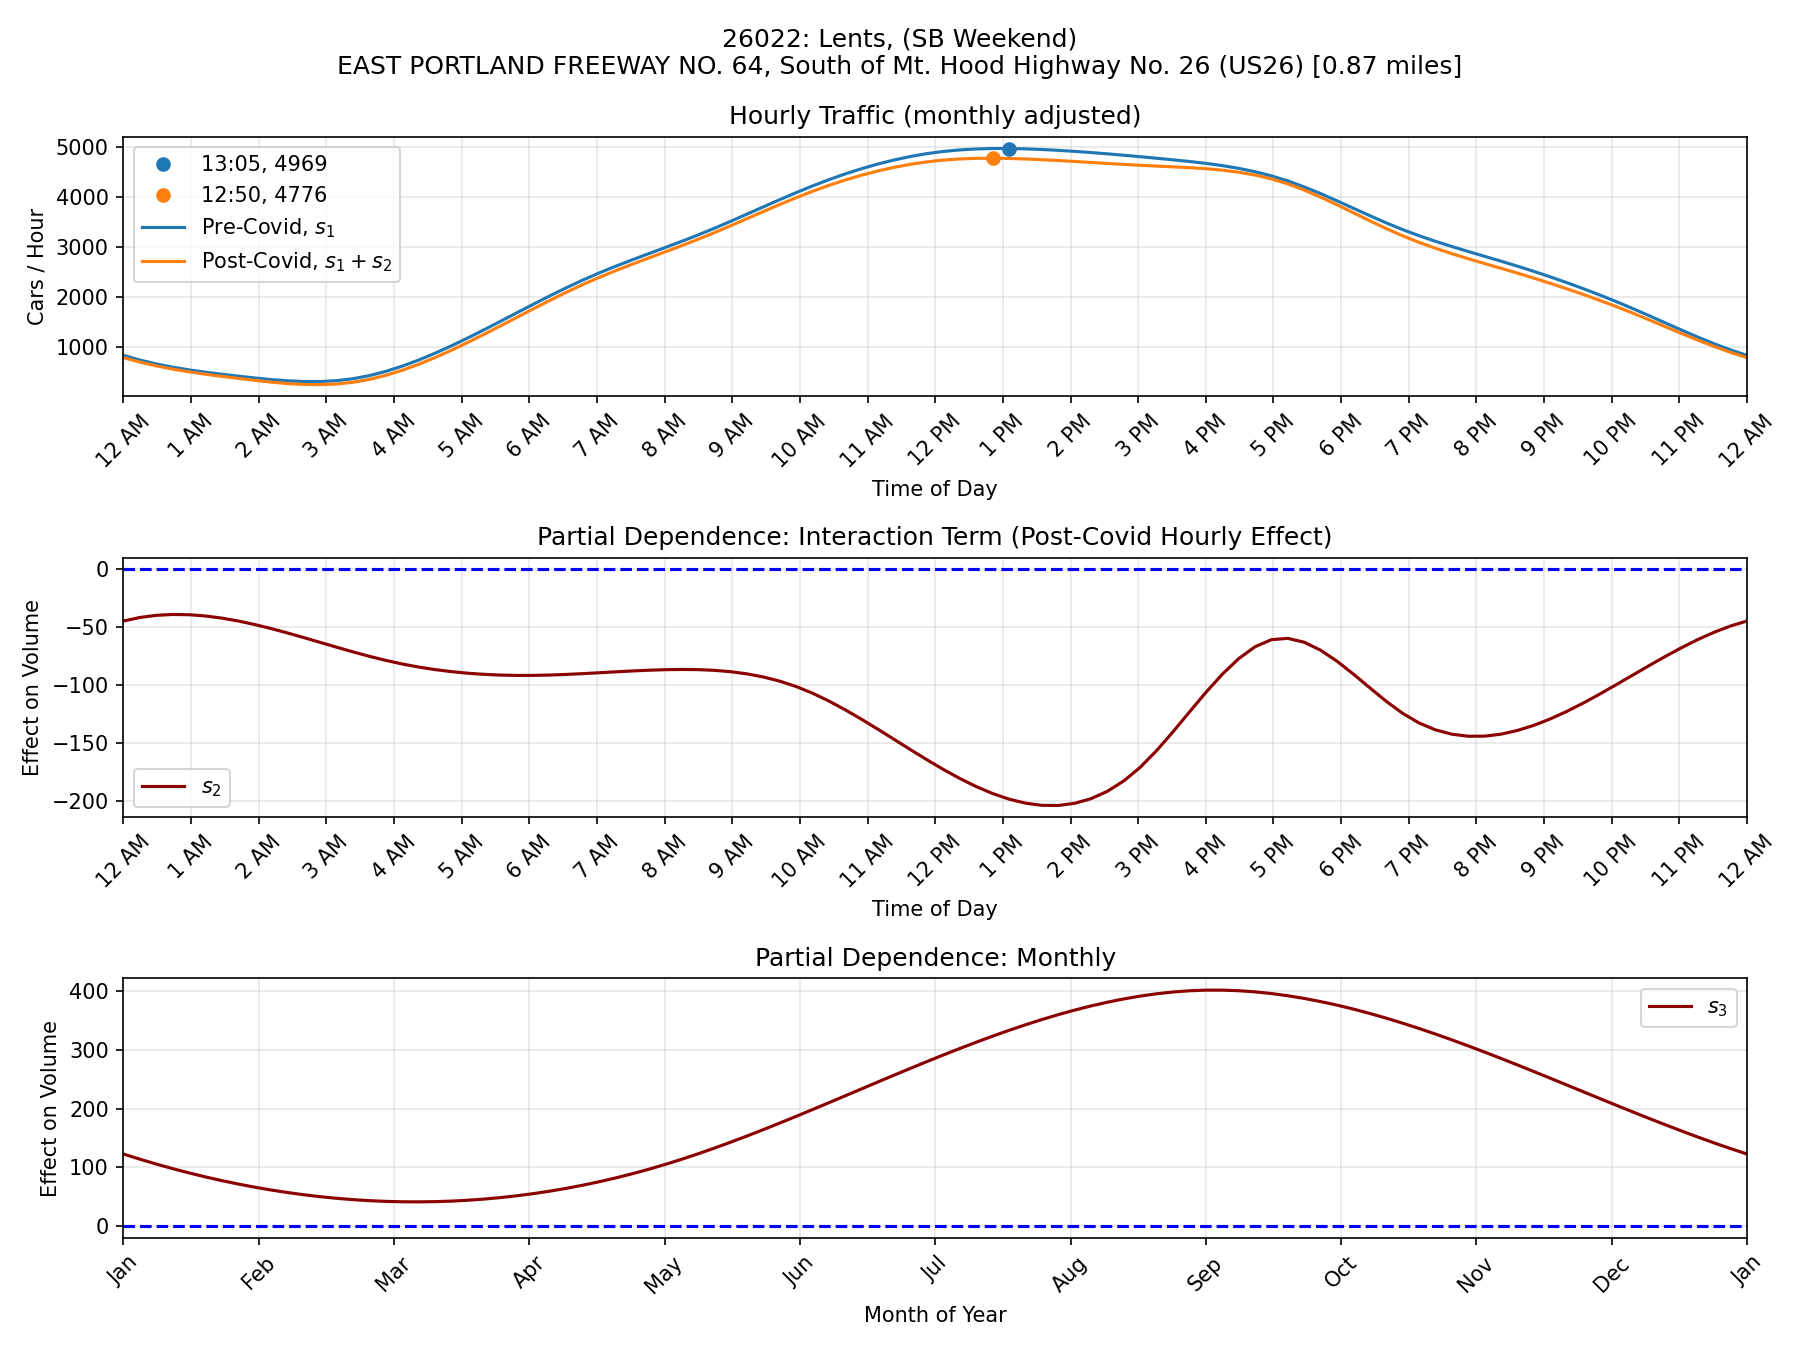
\includegraphics[width=\textwidth]{26022_Lents_SB_Weekend_gam.png}
	\end{subfigure}
\end{figure}

\begin{figure}[H]
	\centering
	\begin{subfigure}[b]{0.45\textwidth}
		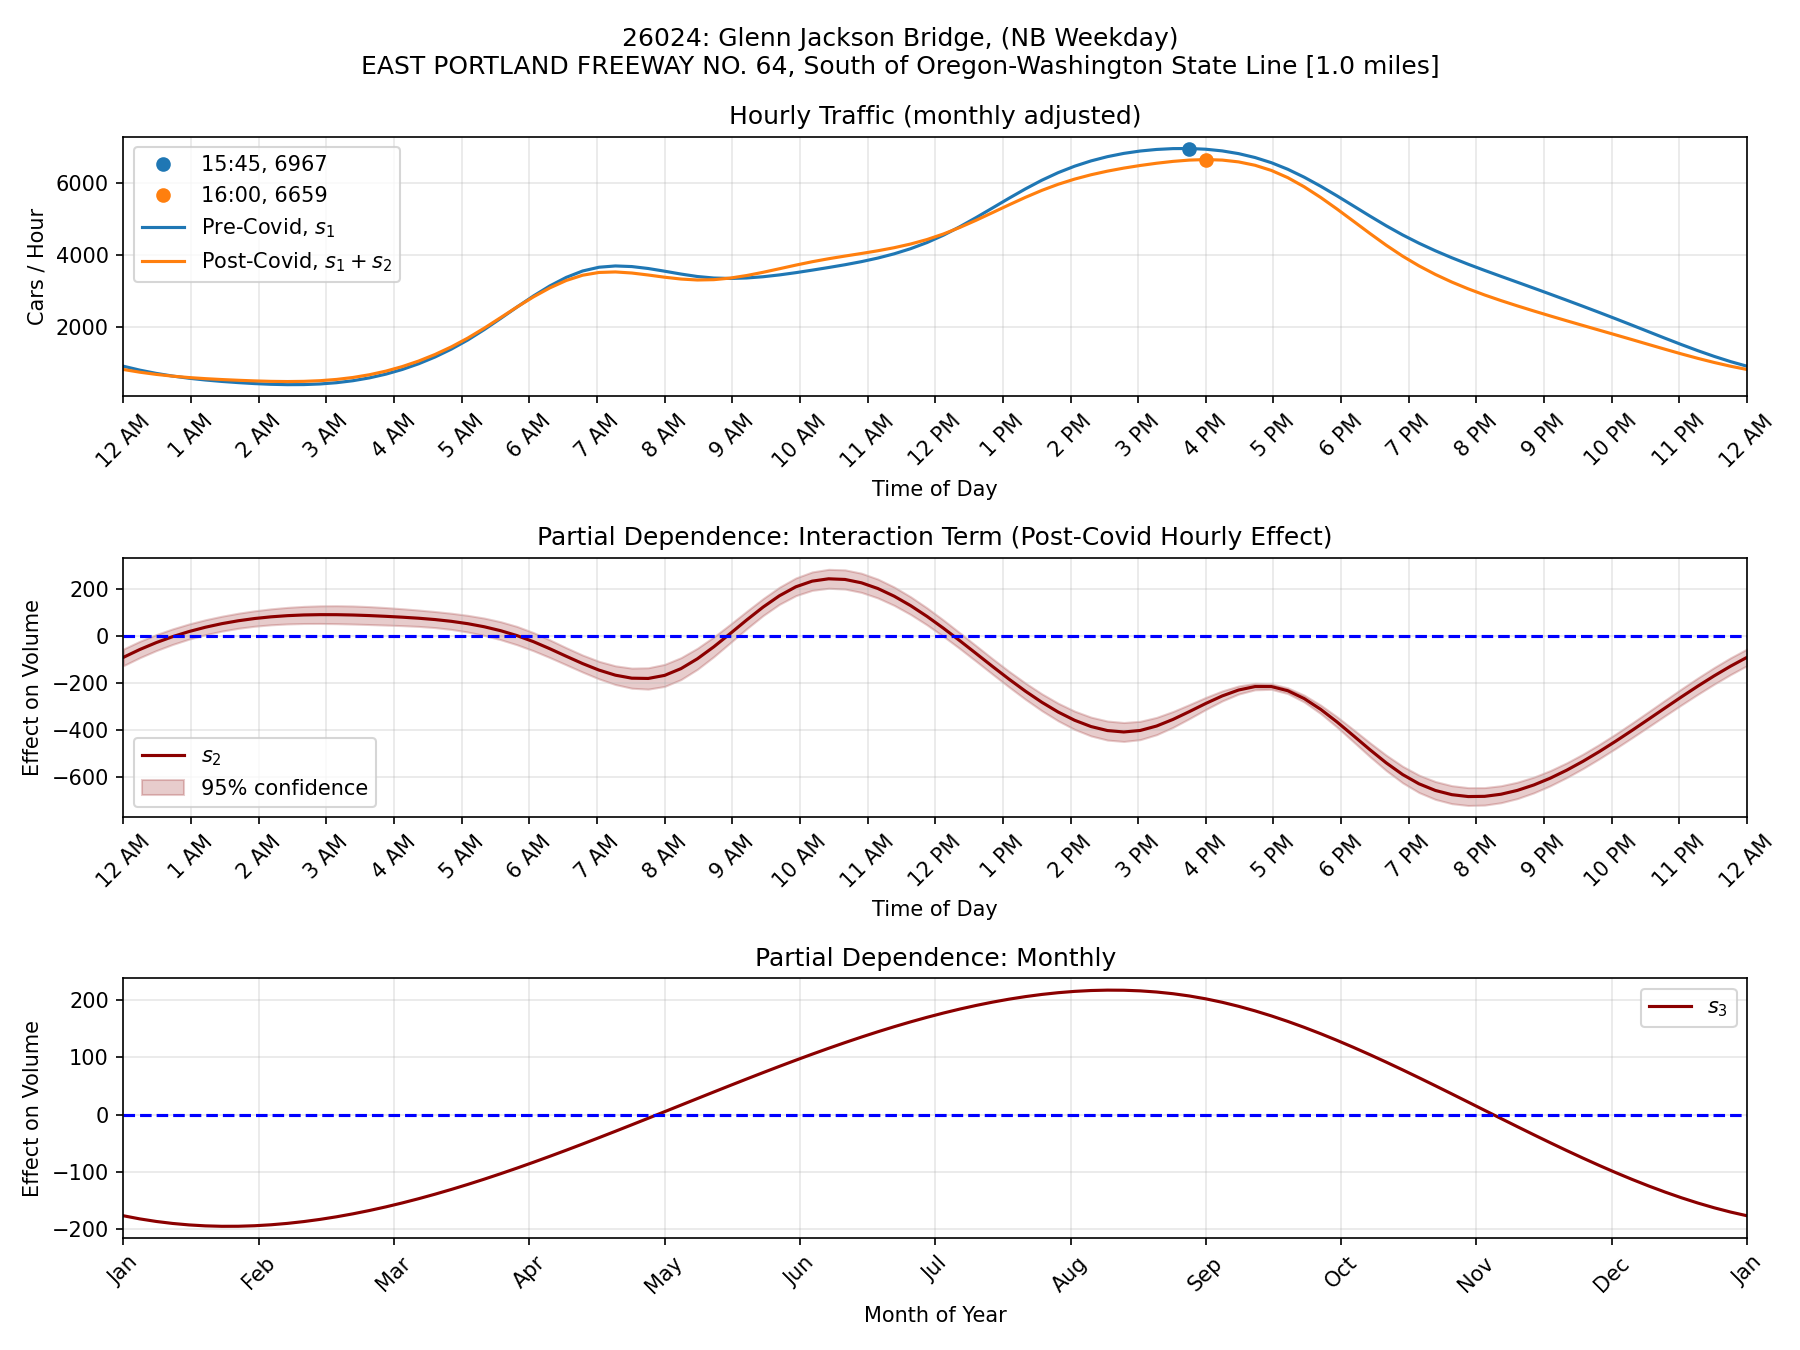
\includegraphics[width=\textwidth]{26024_Glenn-Jackson-Bridge_NB_Weekday_gam.png}
	\end{subfigure}
	\hfill
	\begin{subfigure}[b]{0.45\textwidth}
		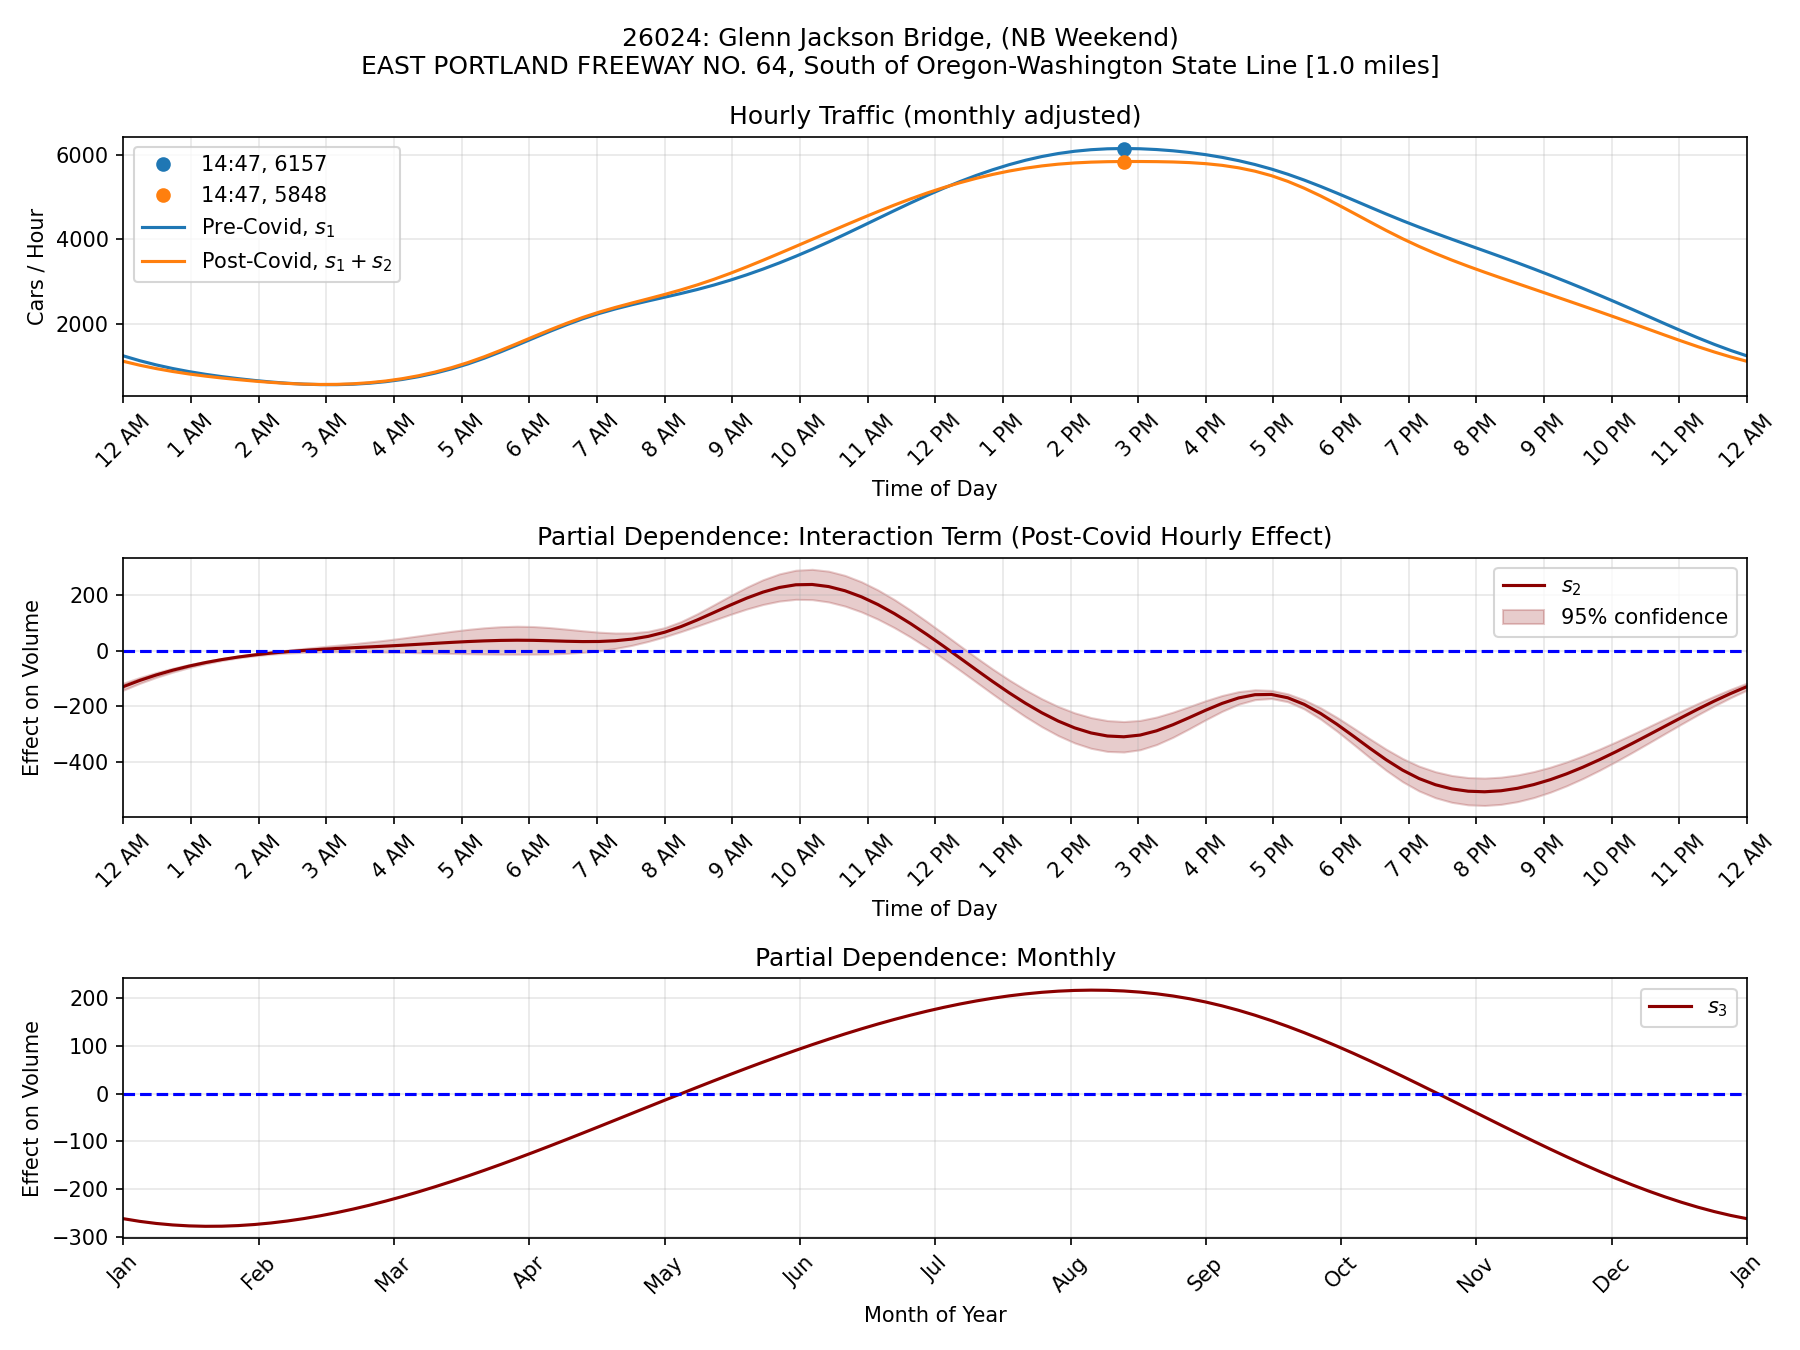
\includegraphics[width=\textwidth]{26024_Glenn-Jackson-Bridge_NB_Weekend_gam.png}
	\end{subfigure}

	\begin{subfigure}[b]{0.45\textwidth}
		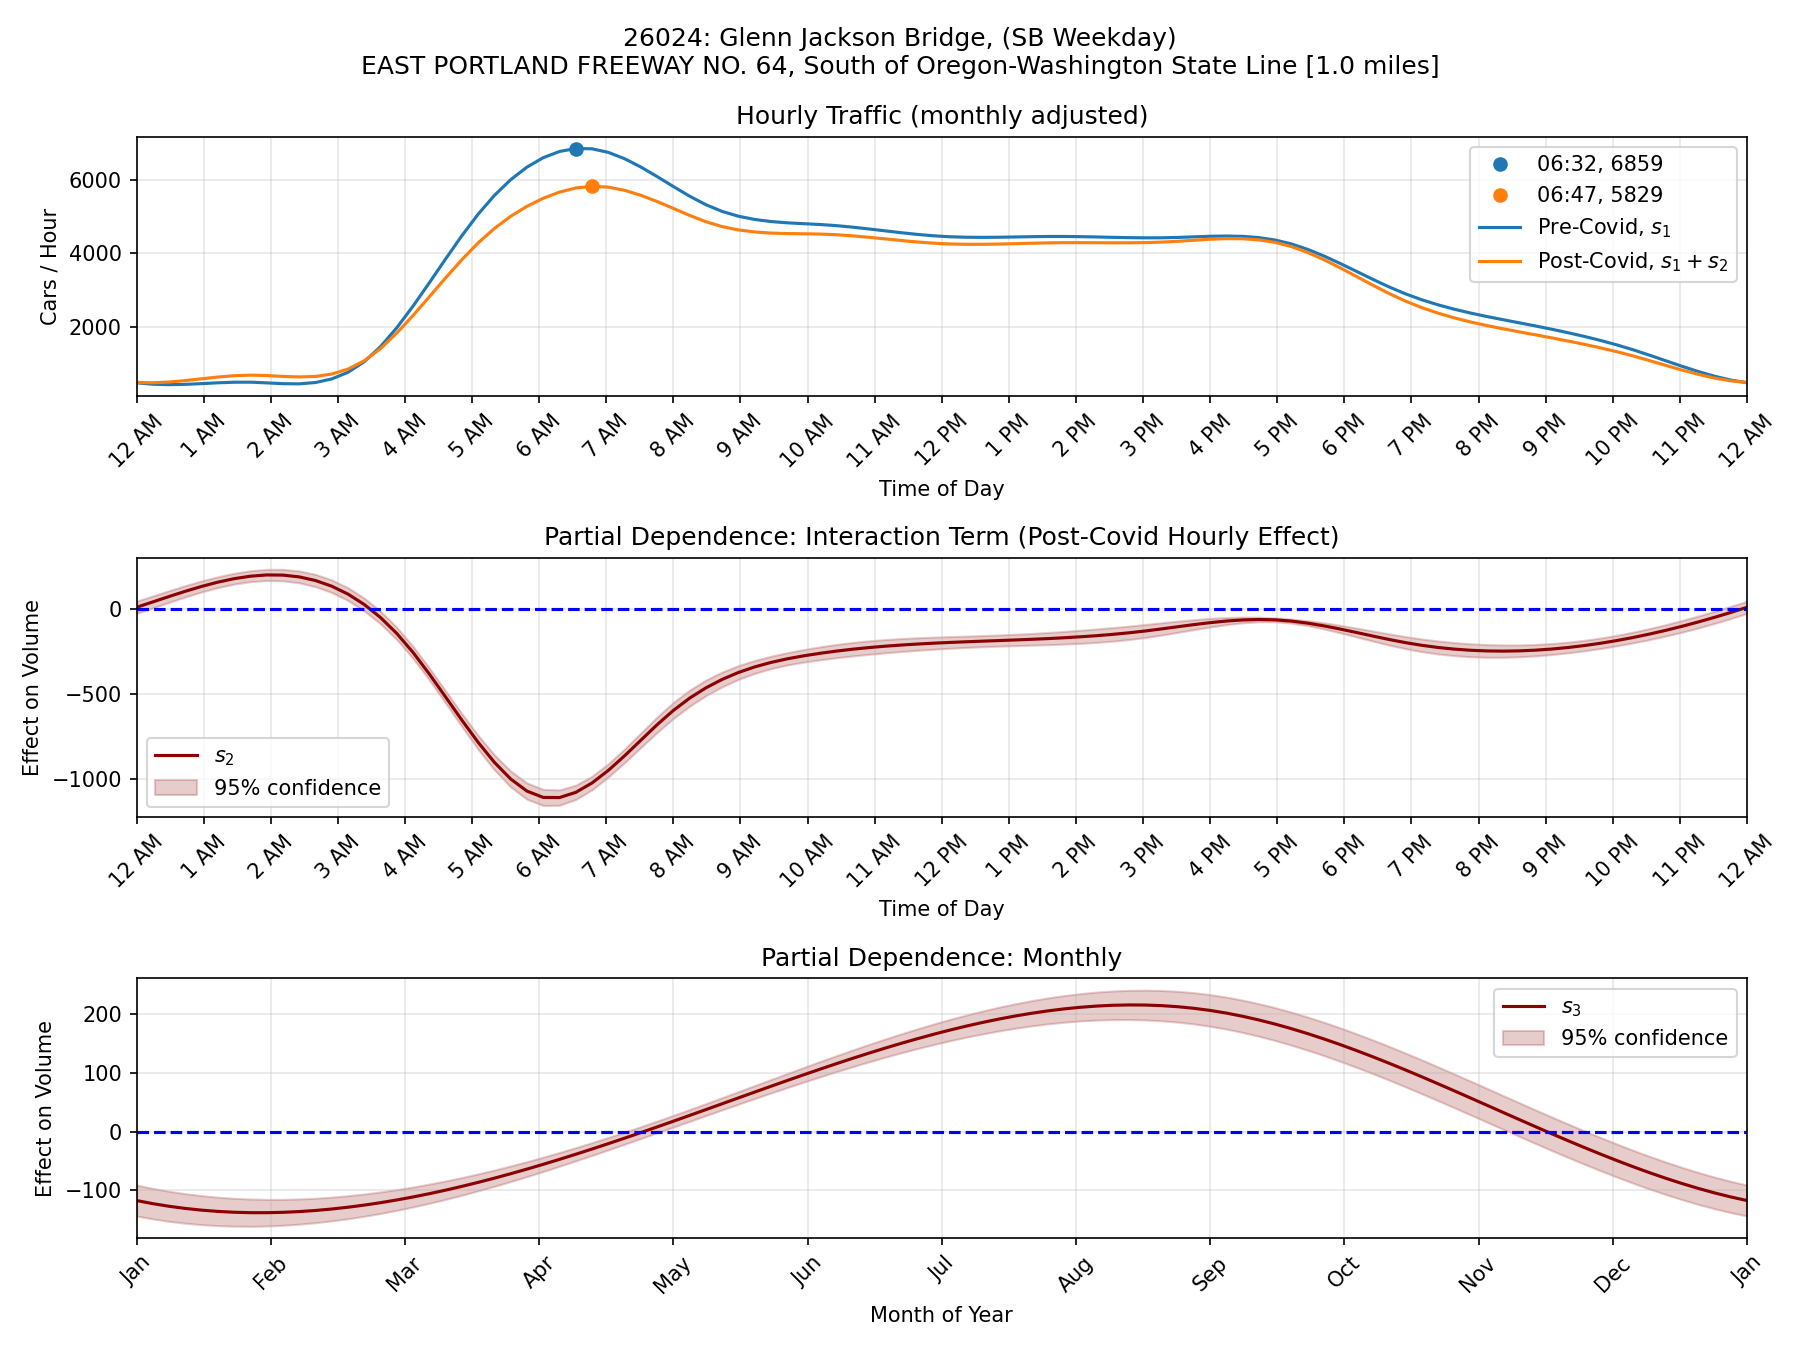
\includegraphics[width=\textwidth]{26024_Glenn-Jackson-Bridge_SB_Weekday_gam.png}
	\end{subfigure}
	\hfill
	\begin{subfigure}[b]{0.45\textwidth}
		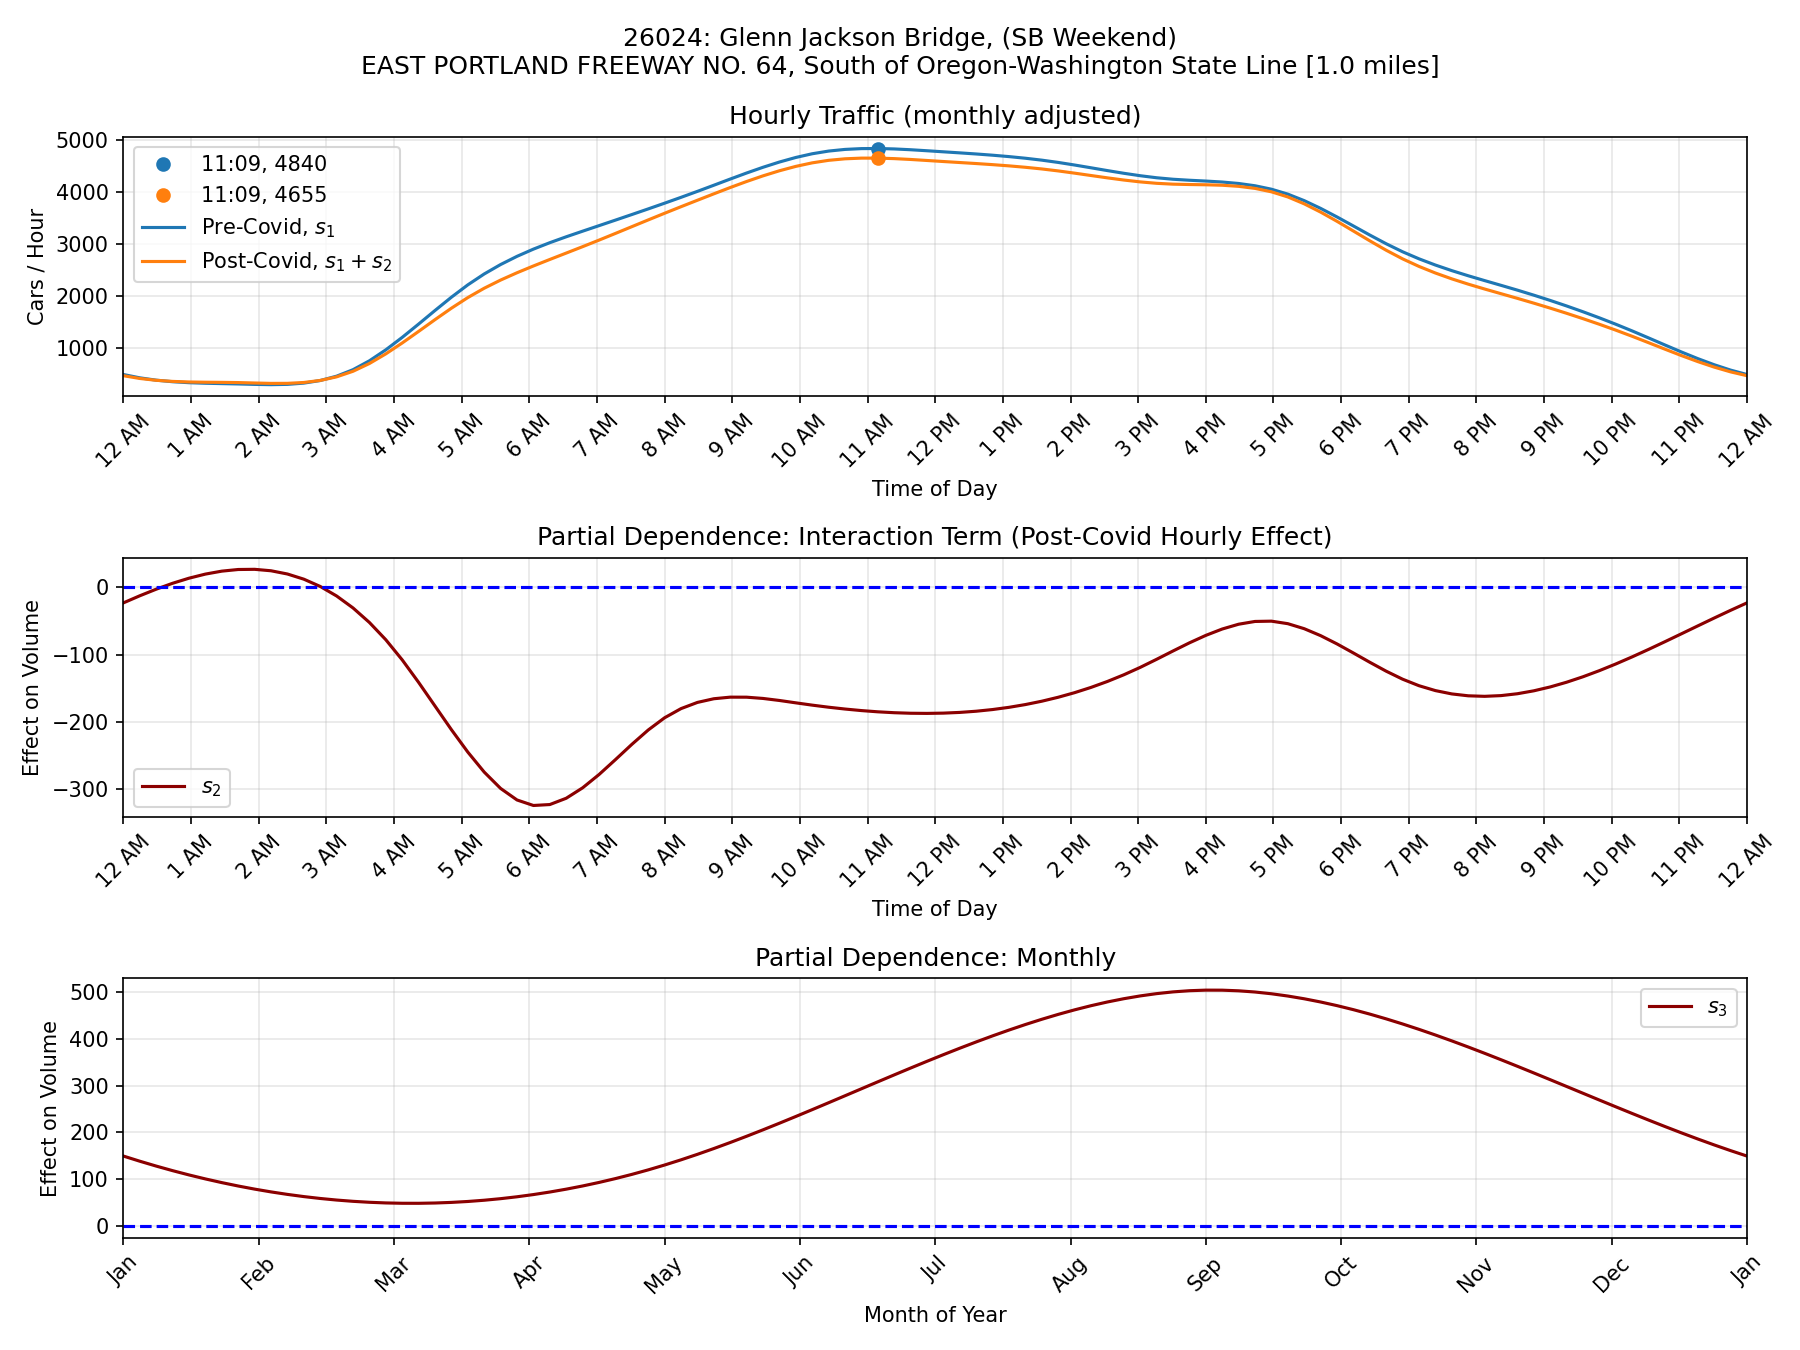
\includegraphics[width=\textwidth]{26024_Glenn-Jackson-Bridge_SB_Weekend_gam.png}
	\end{subfigure}
\end{figure}

\begin{figure}[H]
	\centering
	\begin{subfigure}[b]{0.45\textwidth}
		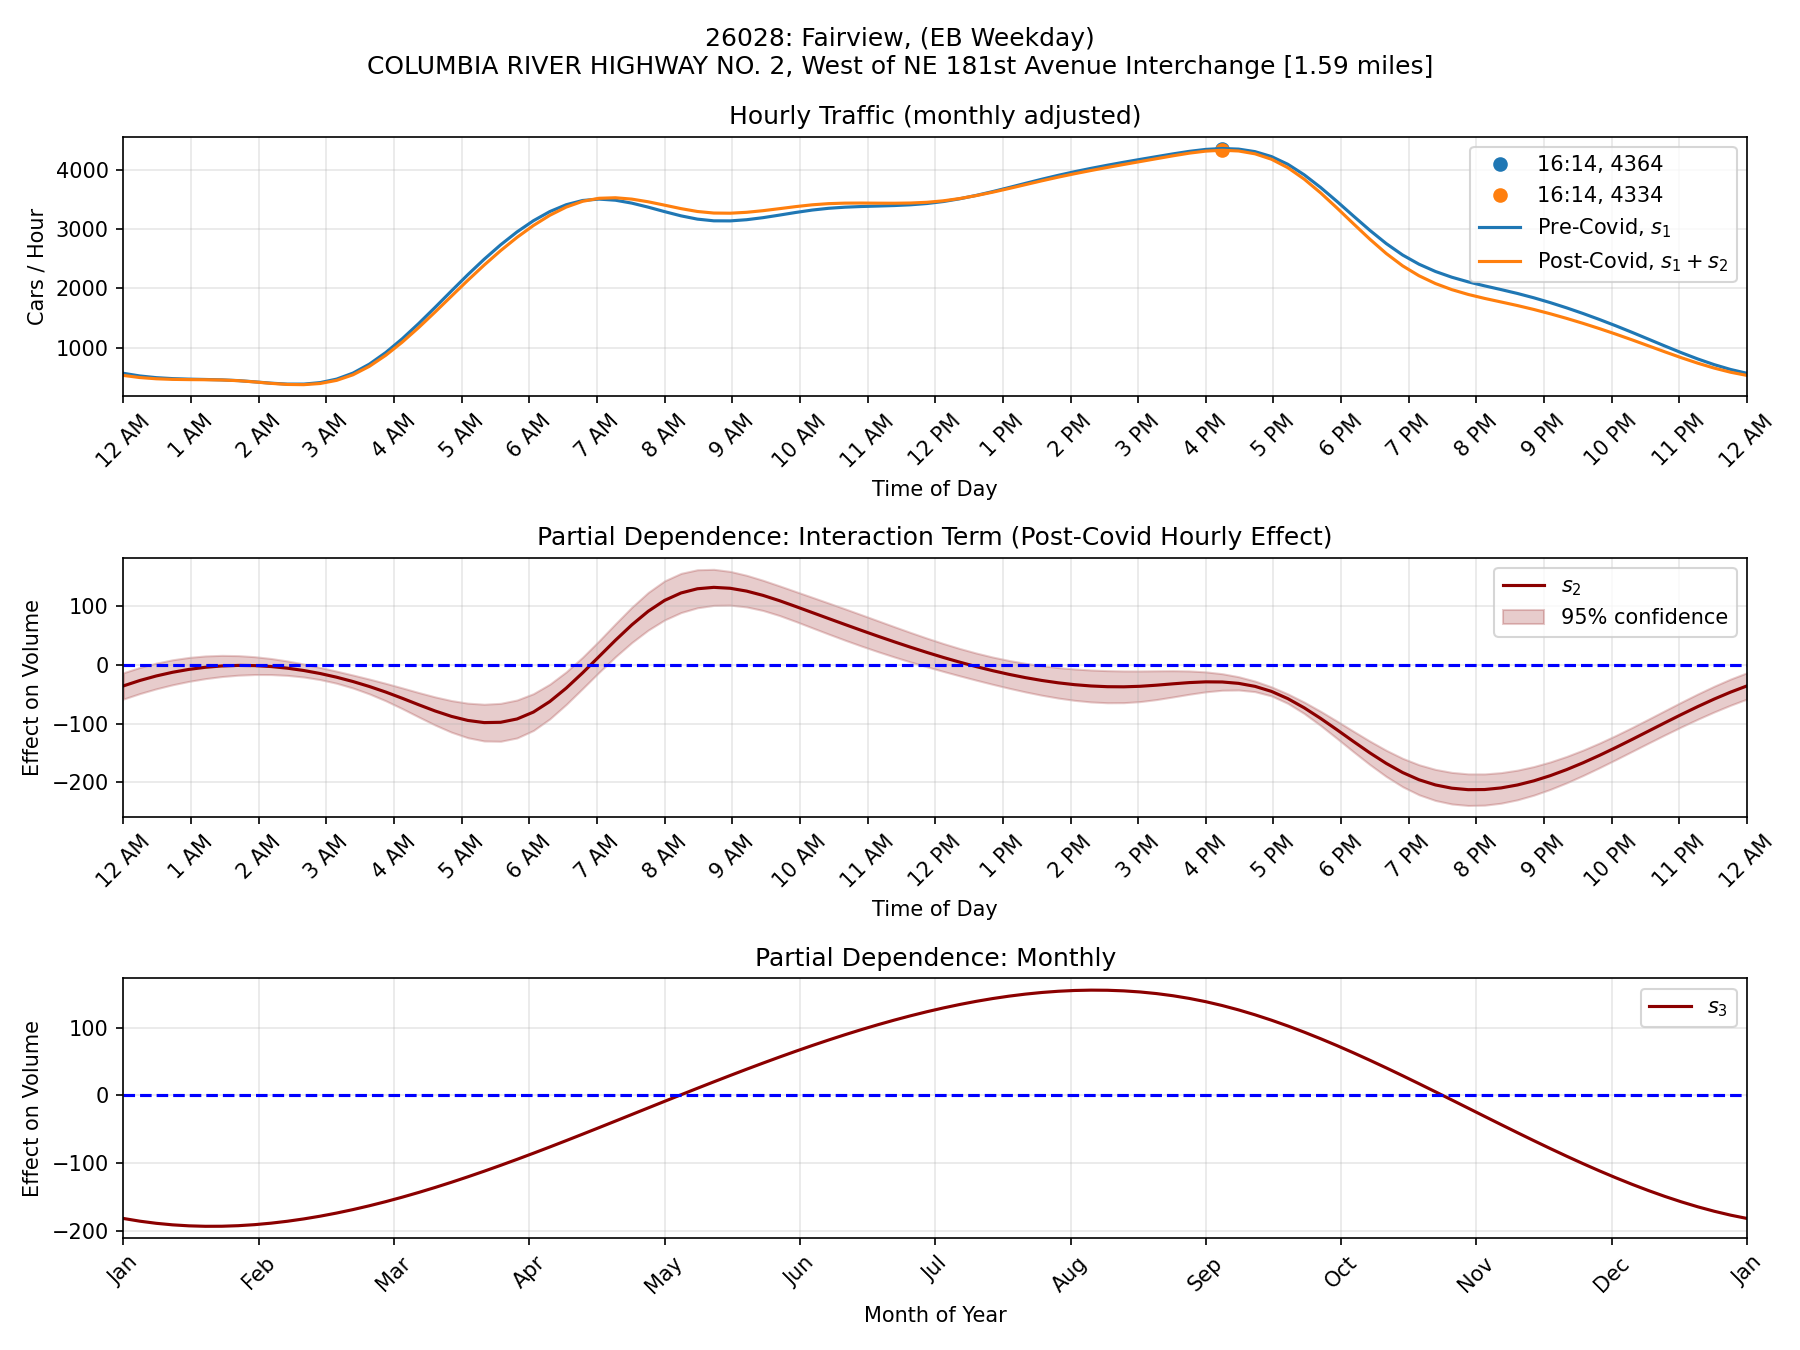
\includegraphics[width=\textwidth]{26028_Fairview_EB_Weekday_gam.png}
	\end{subfigure}
	\hfill
	\begin{subfigure}[b]{0.45\textwidth}
		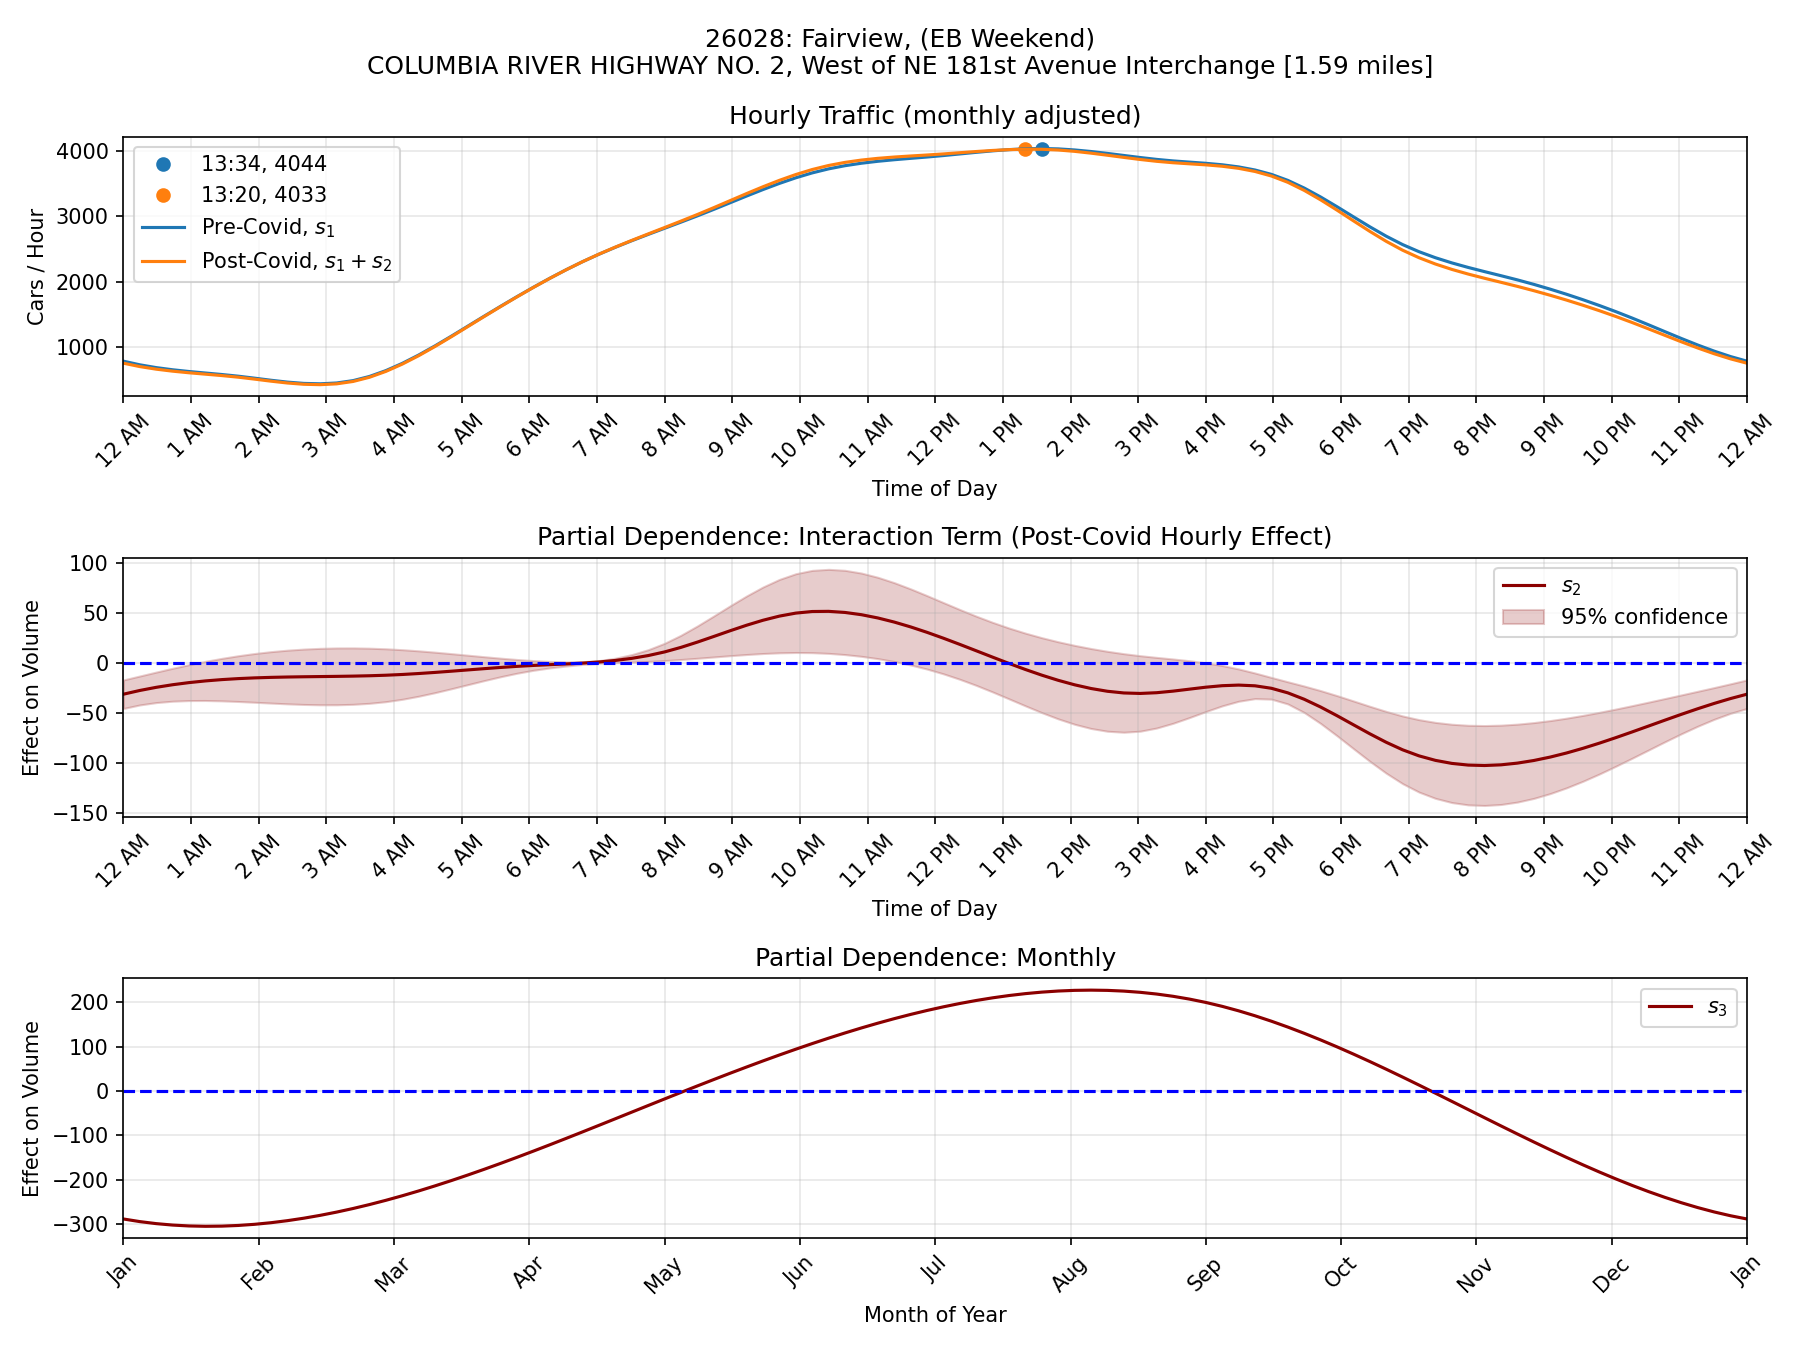
\includegraphics[width=\textwidth]{26028_Fairview_EB_Weekend_gam.png}
	\end{subfigure}

	\begin{subfigure}[b]{0.45\textwidth}
		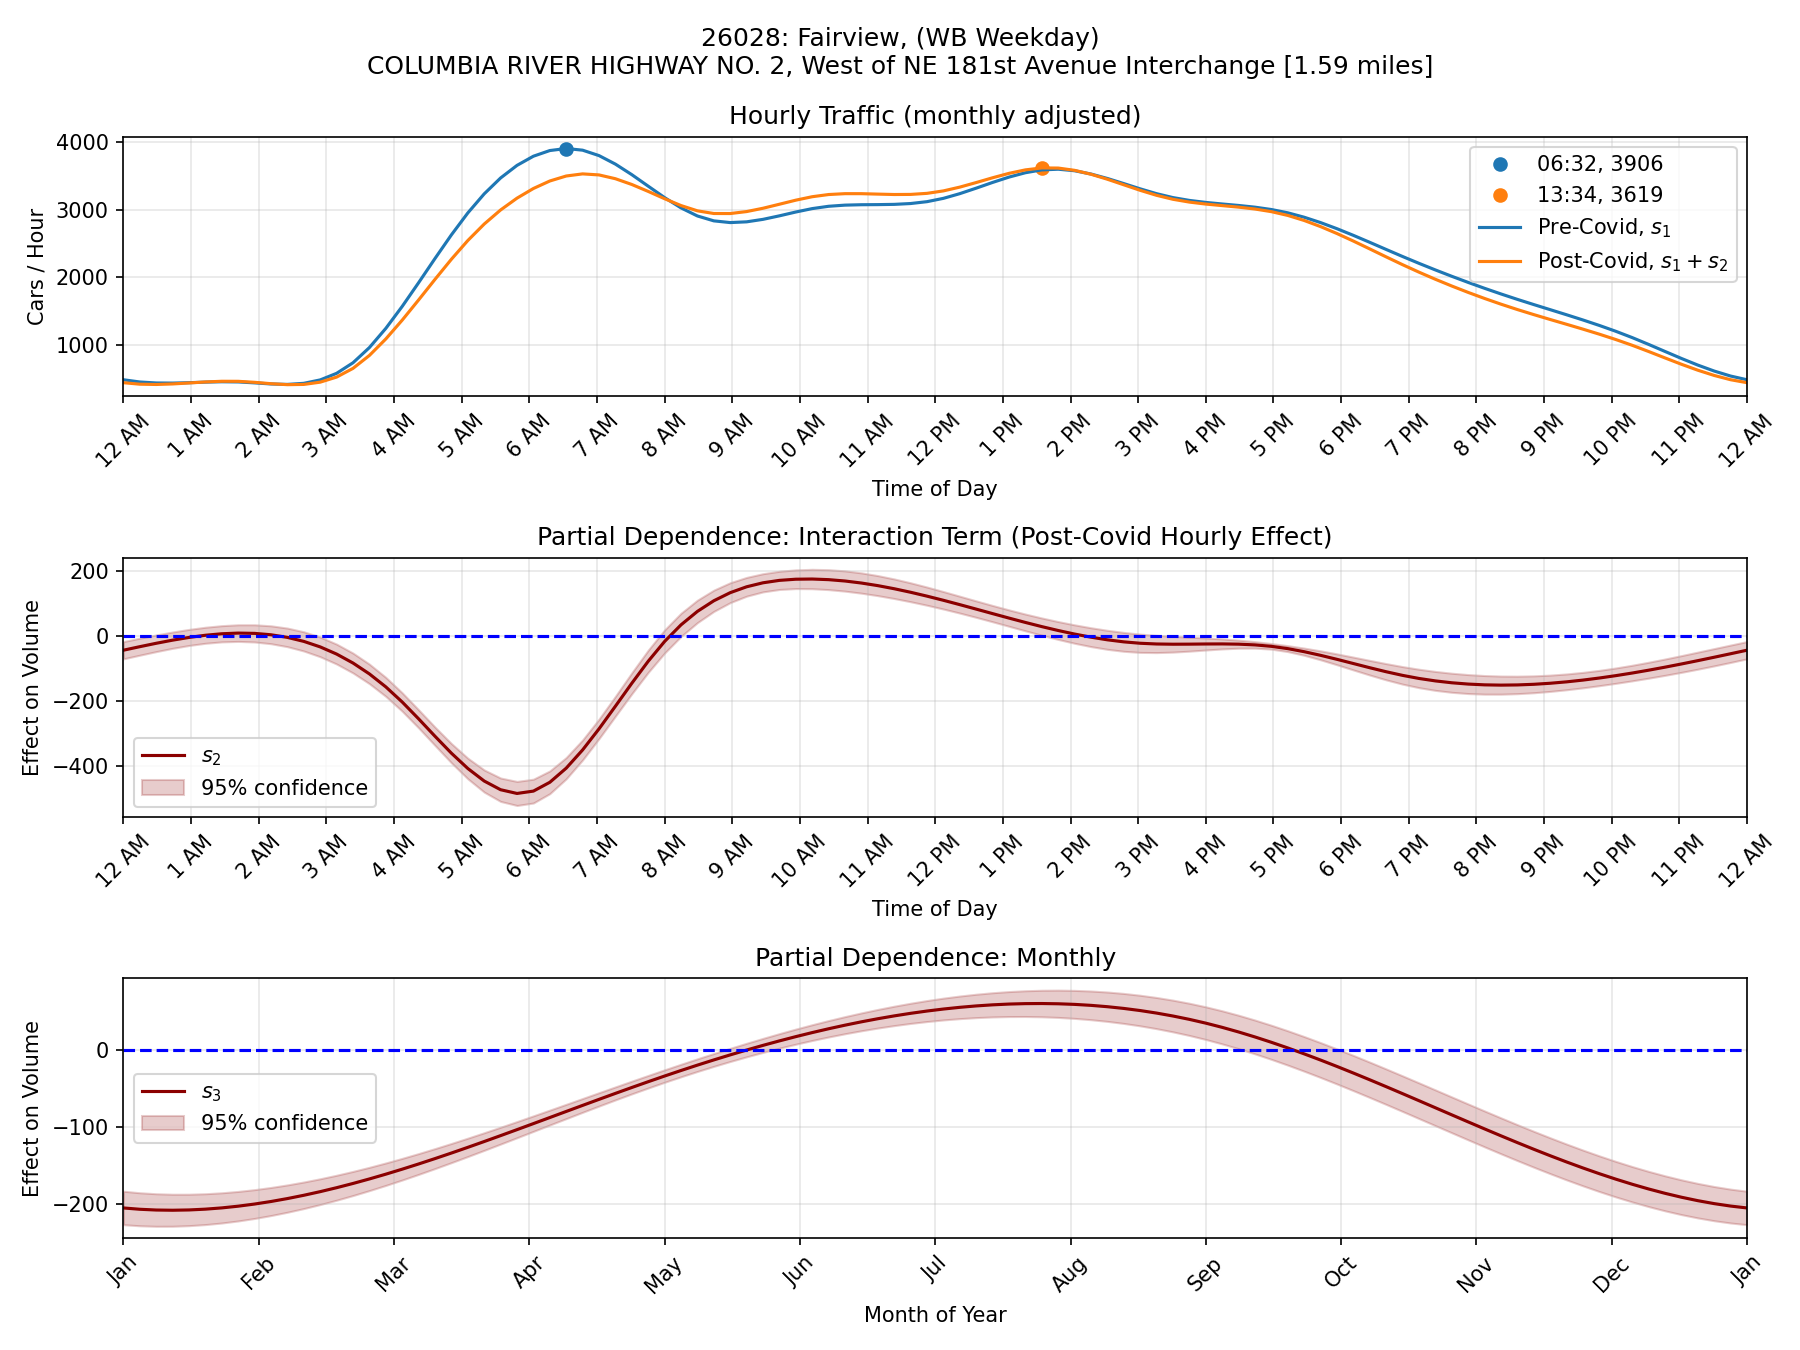
\includegraphics[width=\textwidth]{26028_Fairview_WB_Weekday_gam.png}
	\end{subfigure}
	\hfill
	\begin{subfigure}[b]{0.45\textwidth}
		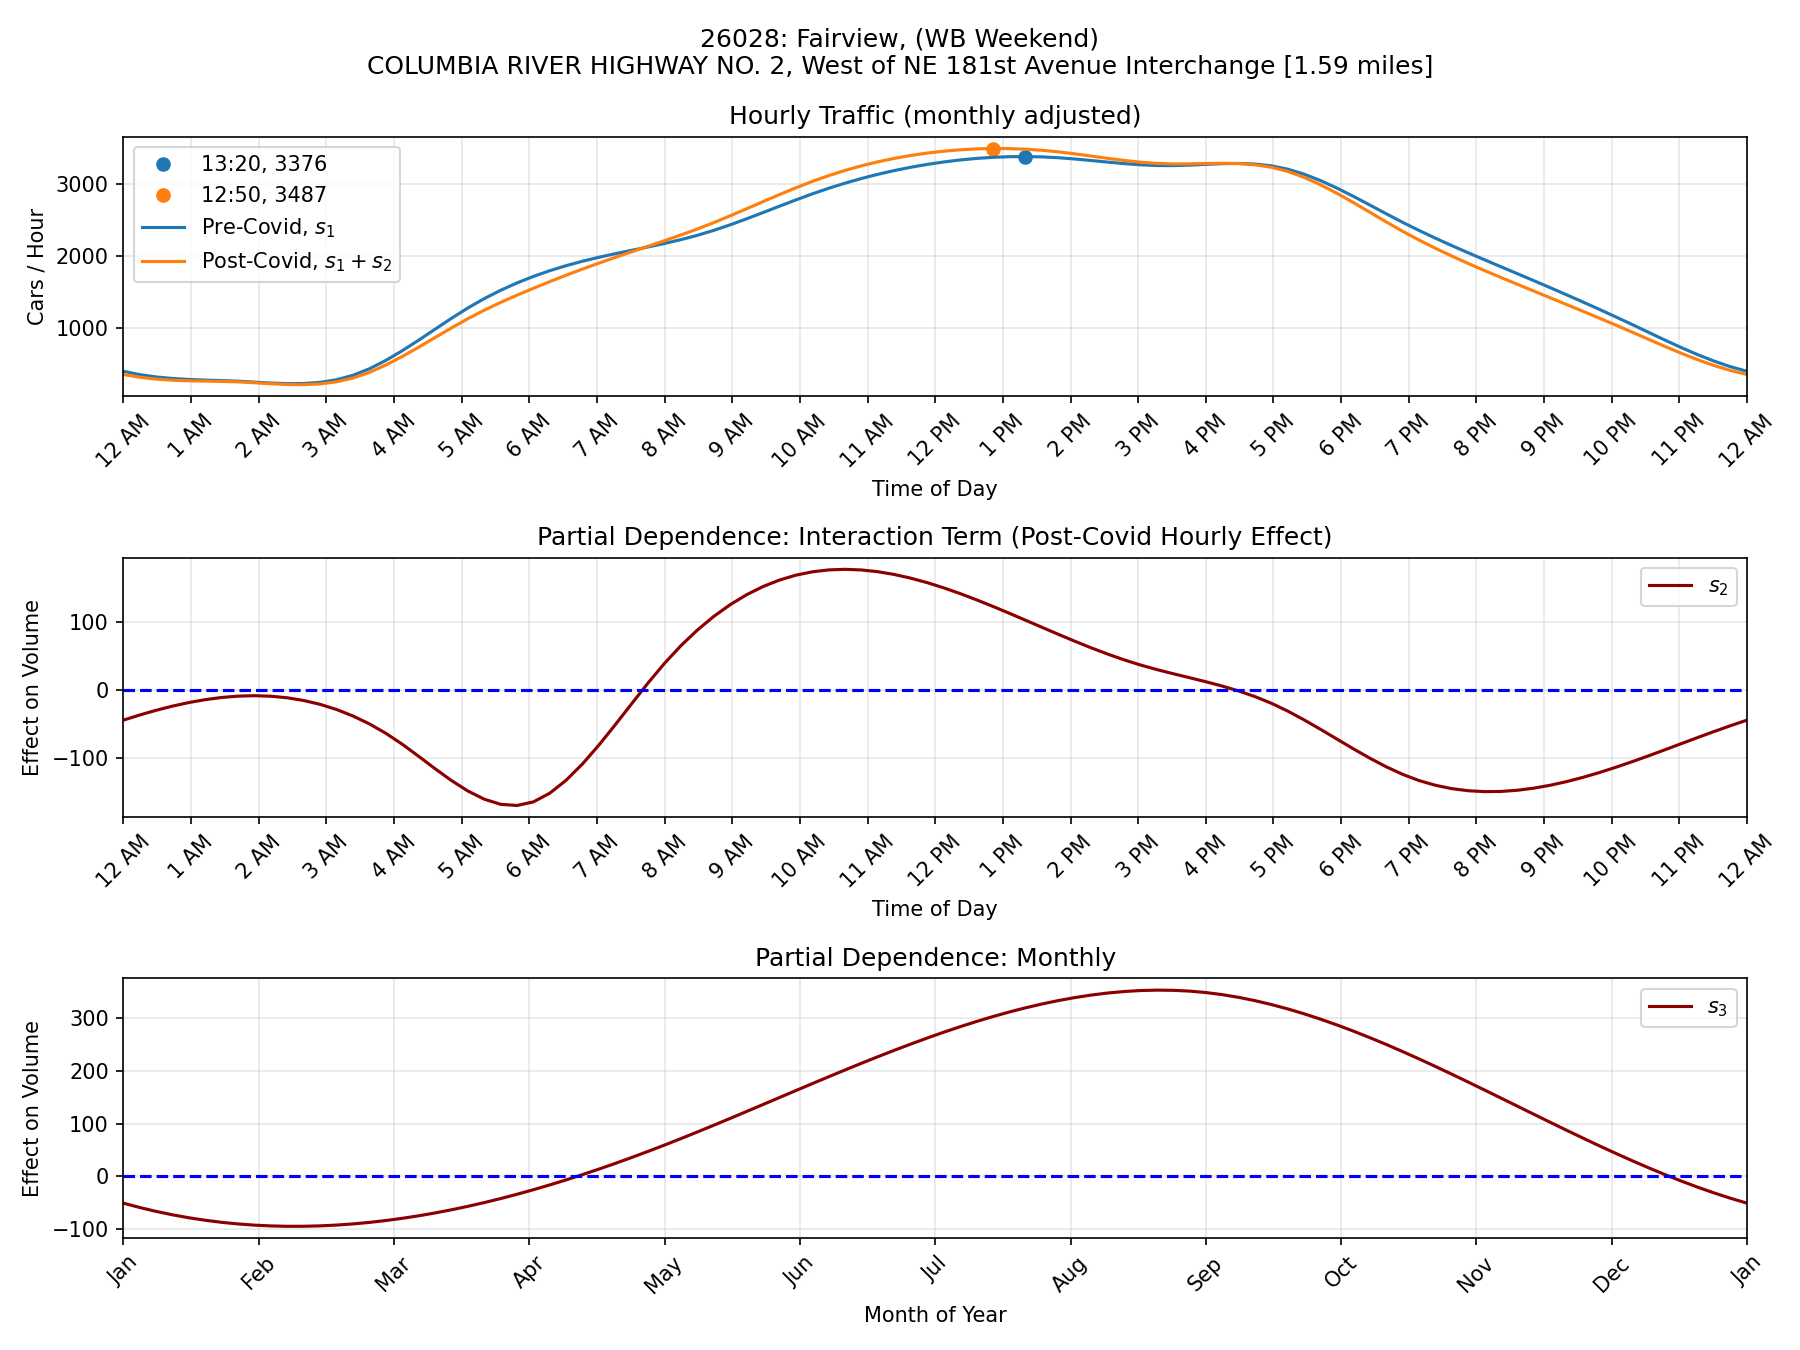
\includegraphics[width=\textwidth]{26028_Fairview_WB_Weekend_gam.png}
	\end{subfigure}
\end{figure}

\begin{figure}[H]
	\centering
	\begin{subfigure}[b]{0.45\textwidth}
		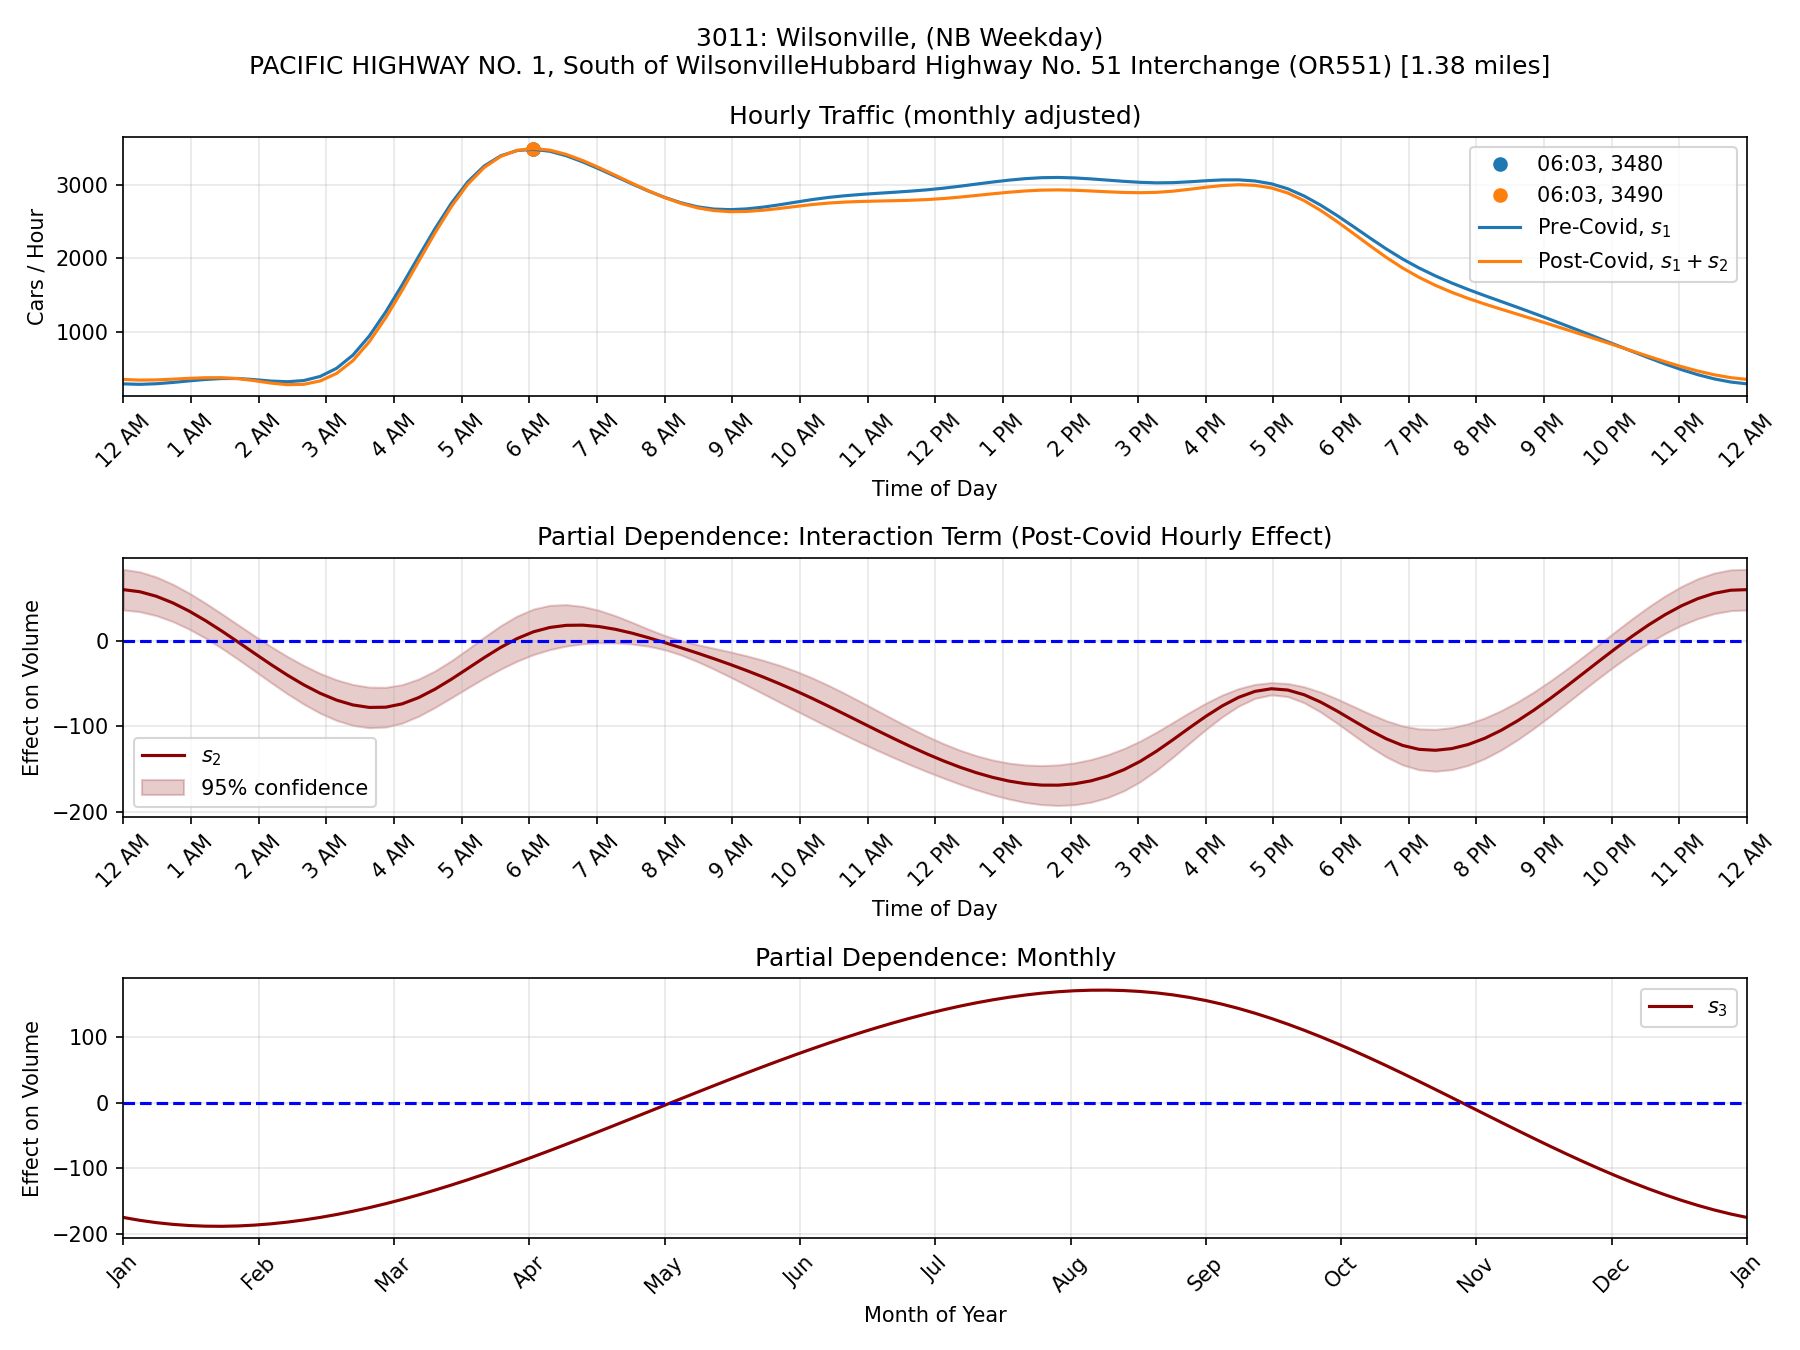
\includegraphics[width=\textwidth]{3011_Wilsonville_NB_Weekday_gam.png}
	\end{subfigure}
	\hfill
	\begin{subfigure}[b]{0.45\textwidth}
		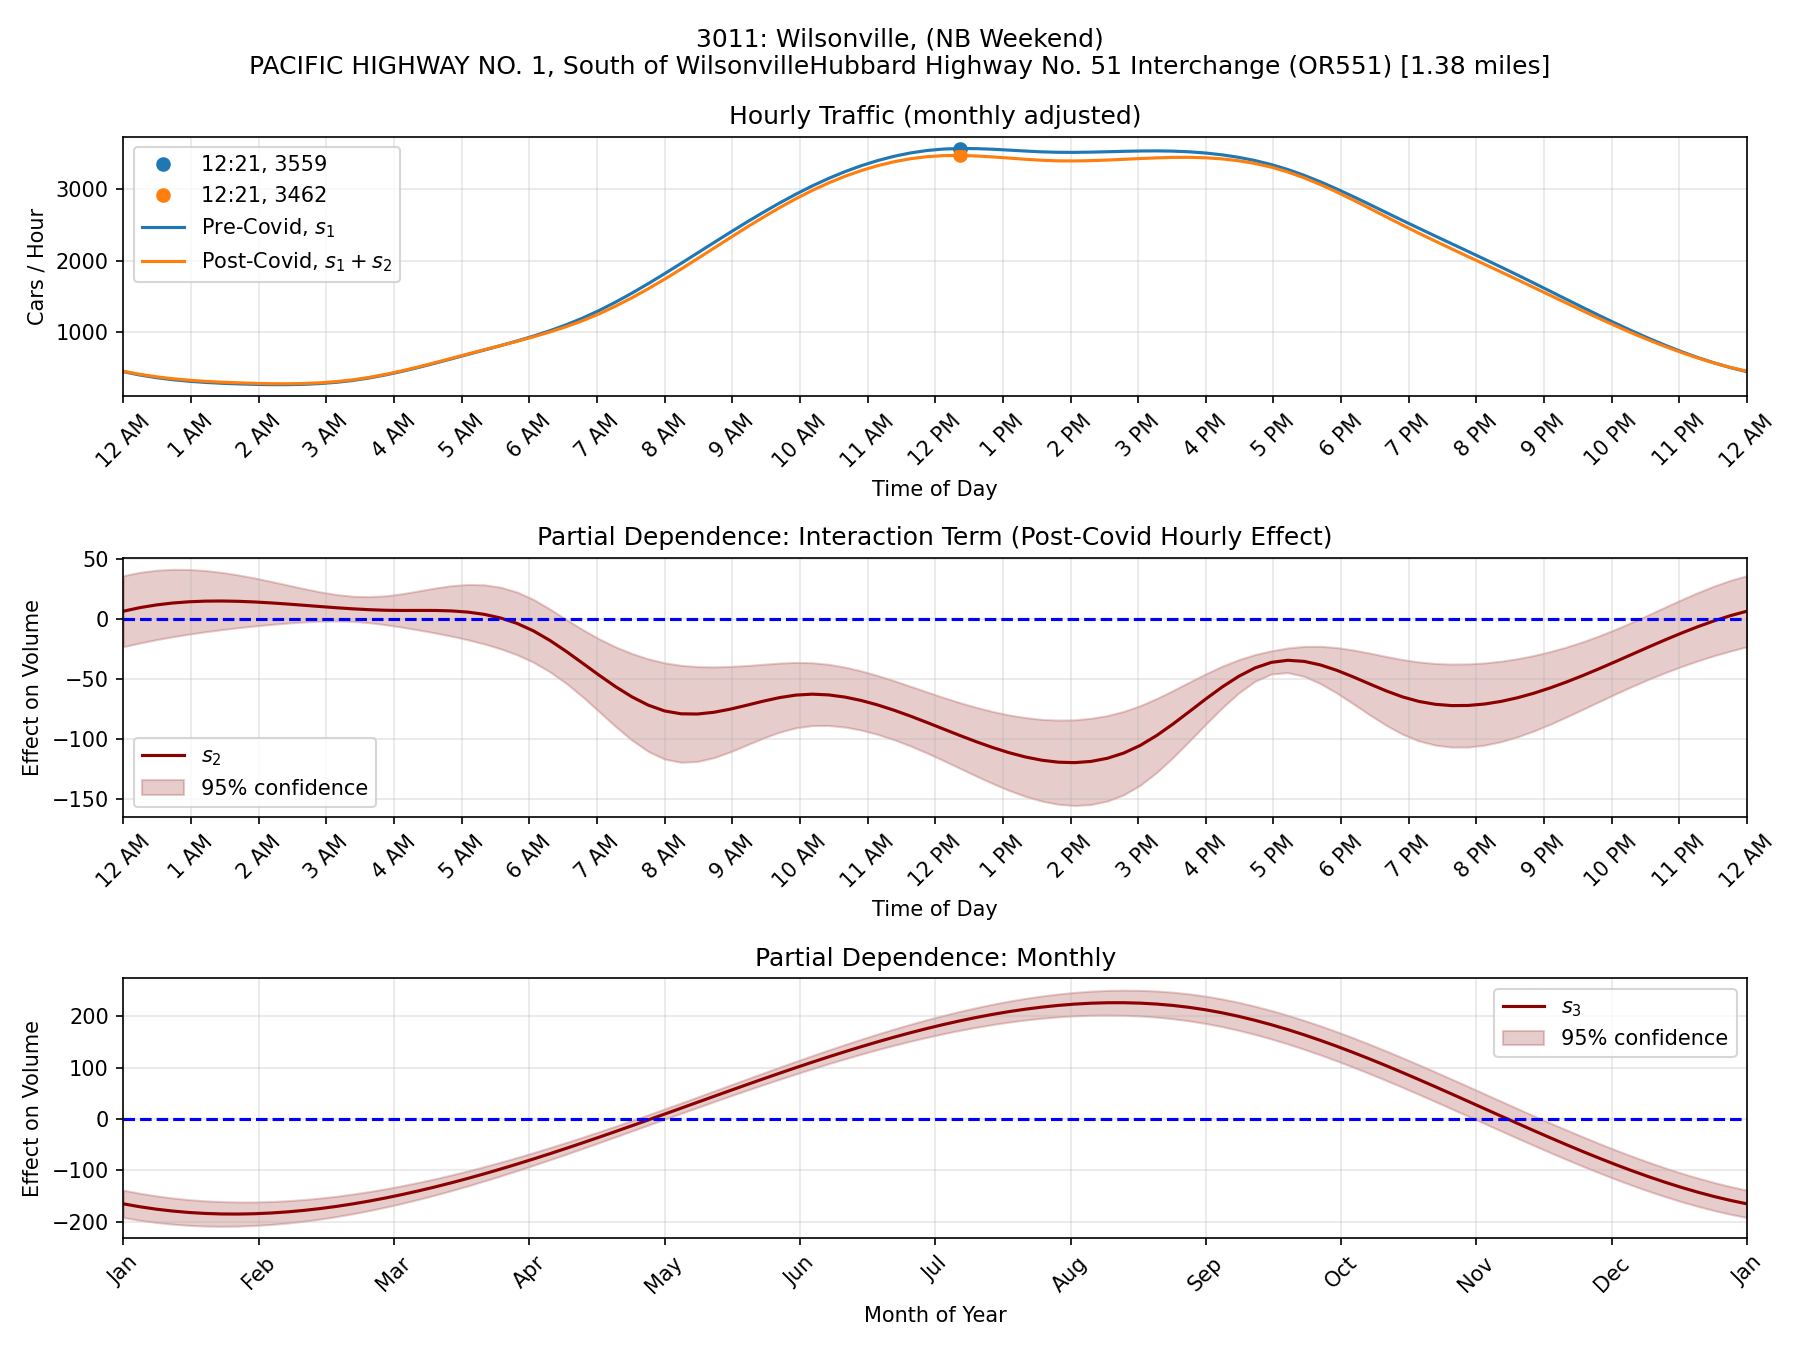
\includegraphics[width=\textwidth]{3011_Wilsonville_NB_Weekend_gam.png}
	\end{subfigure}

	\begin{subfigure}[b]{0.45\textwidth}
		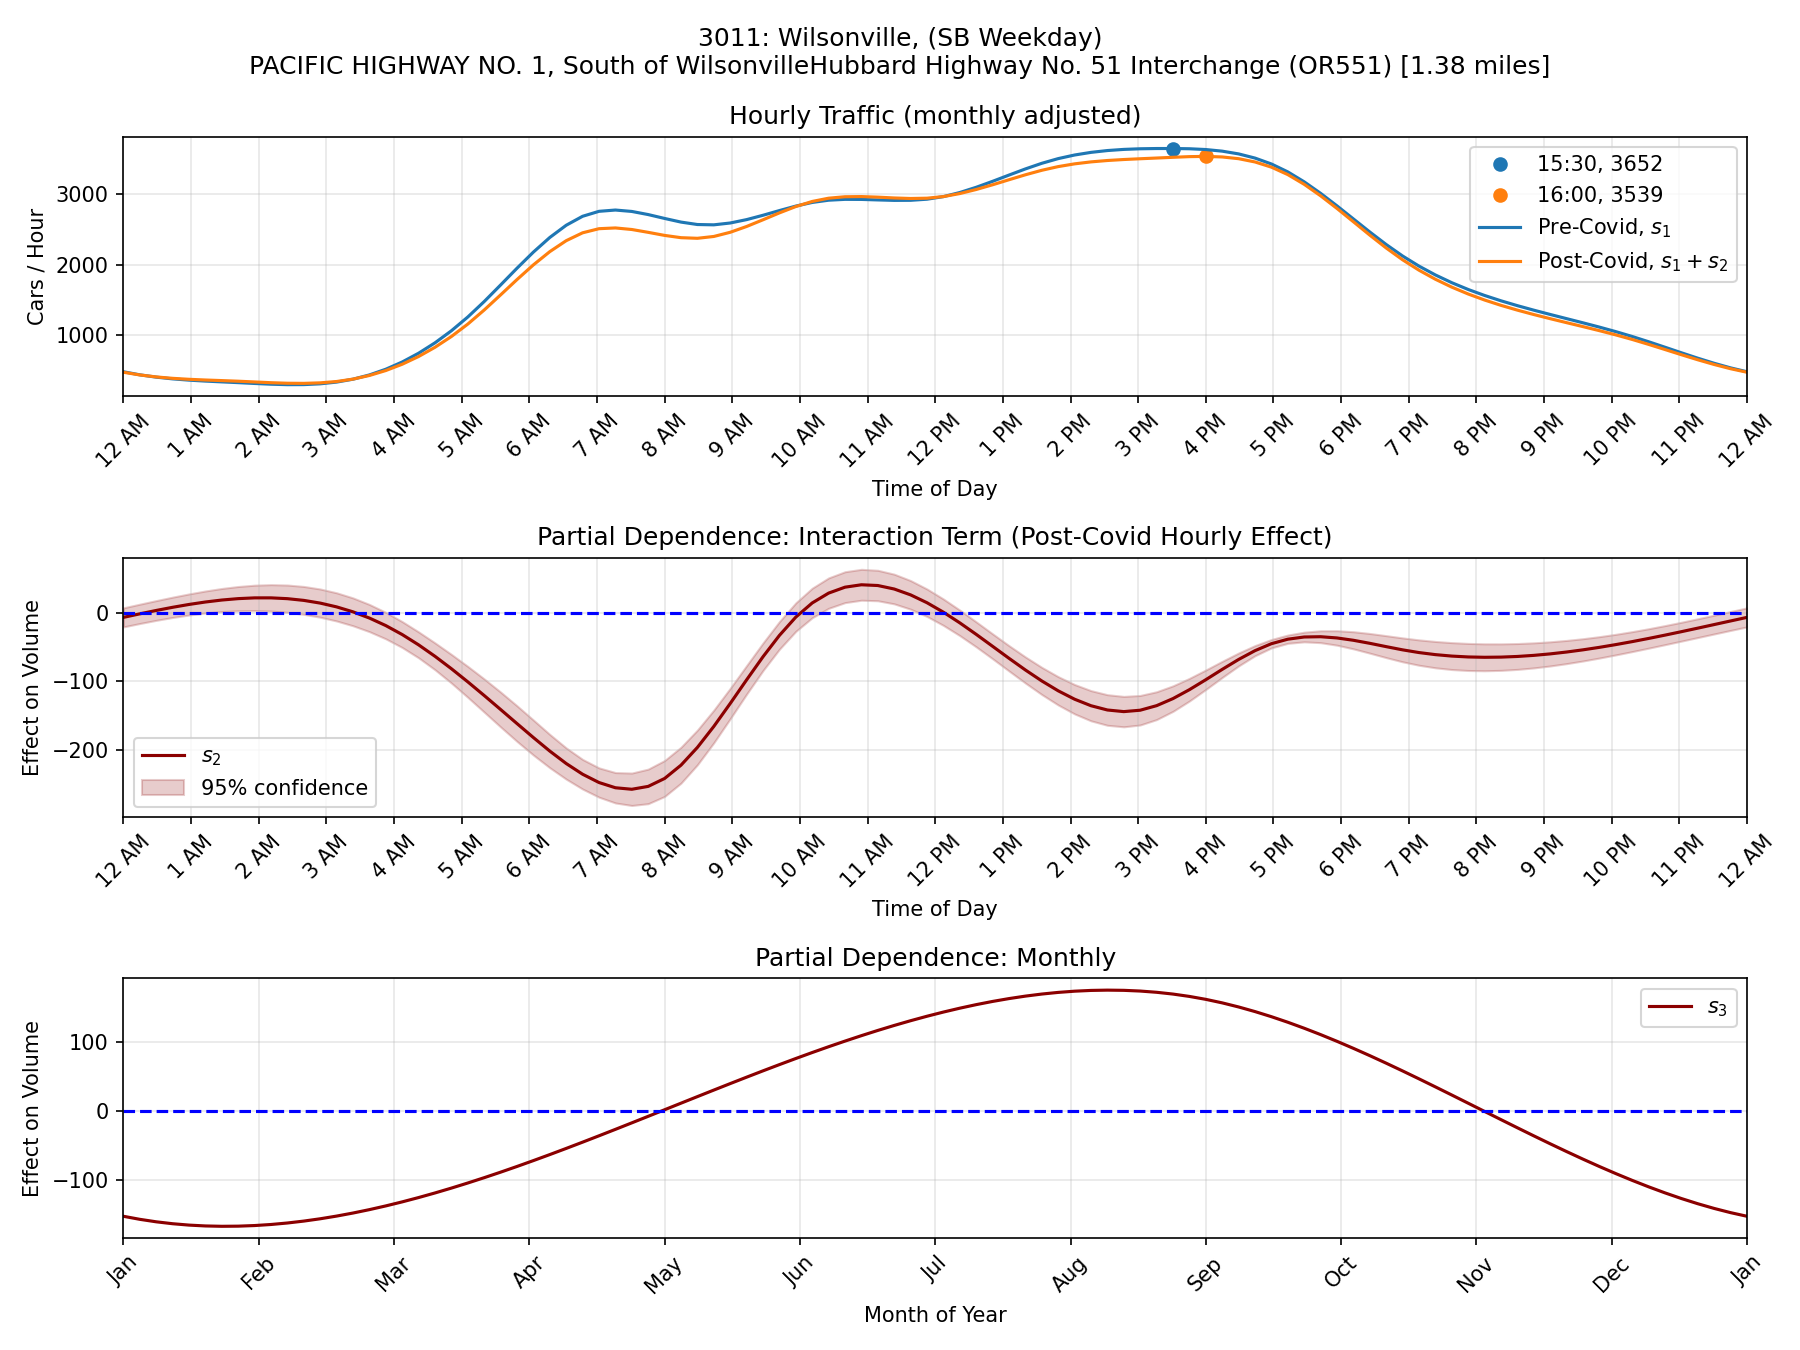
\includegraphics[width=\textwidth]{3011_Wilsonville_SB_Weekday_gam.png}
	\end{subfigure}
	\hfill
	\begin{subfigure}[b]{0.45\textwidth}
		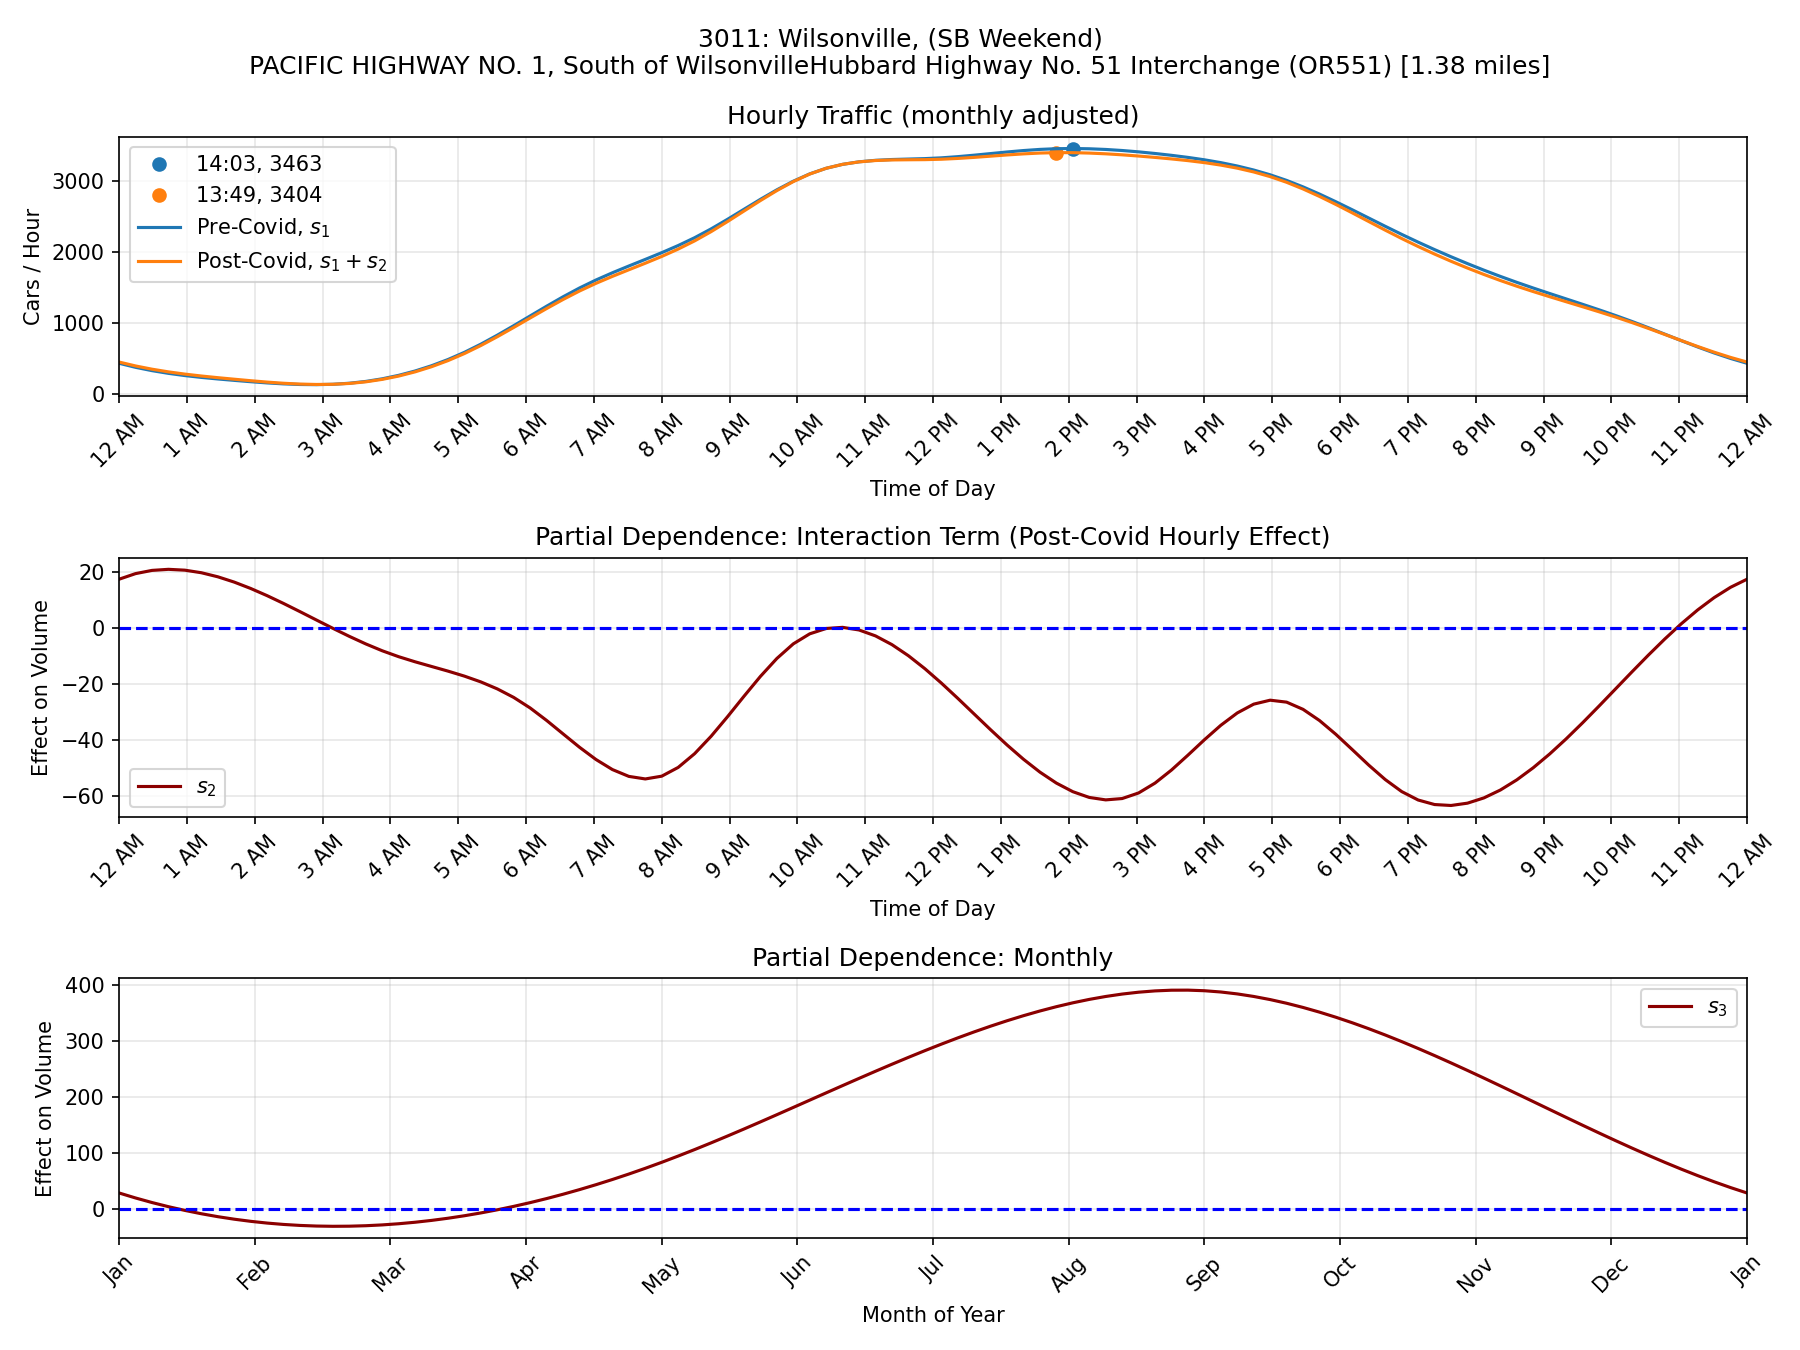
\includegraphics[width=\textwidth]{3011_Wilsonville_SB_Weekend_gam.png}
	\end{subfigure}
\end{figure}

\begin{figure}[H]
	\centering
	\begin{subfigure}[b]{0.45\textwidth}
		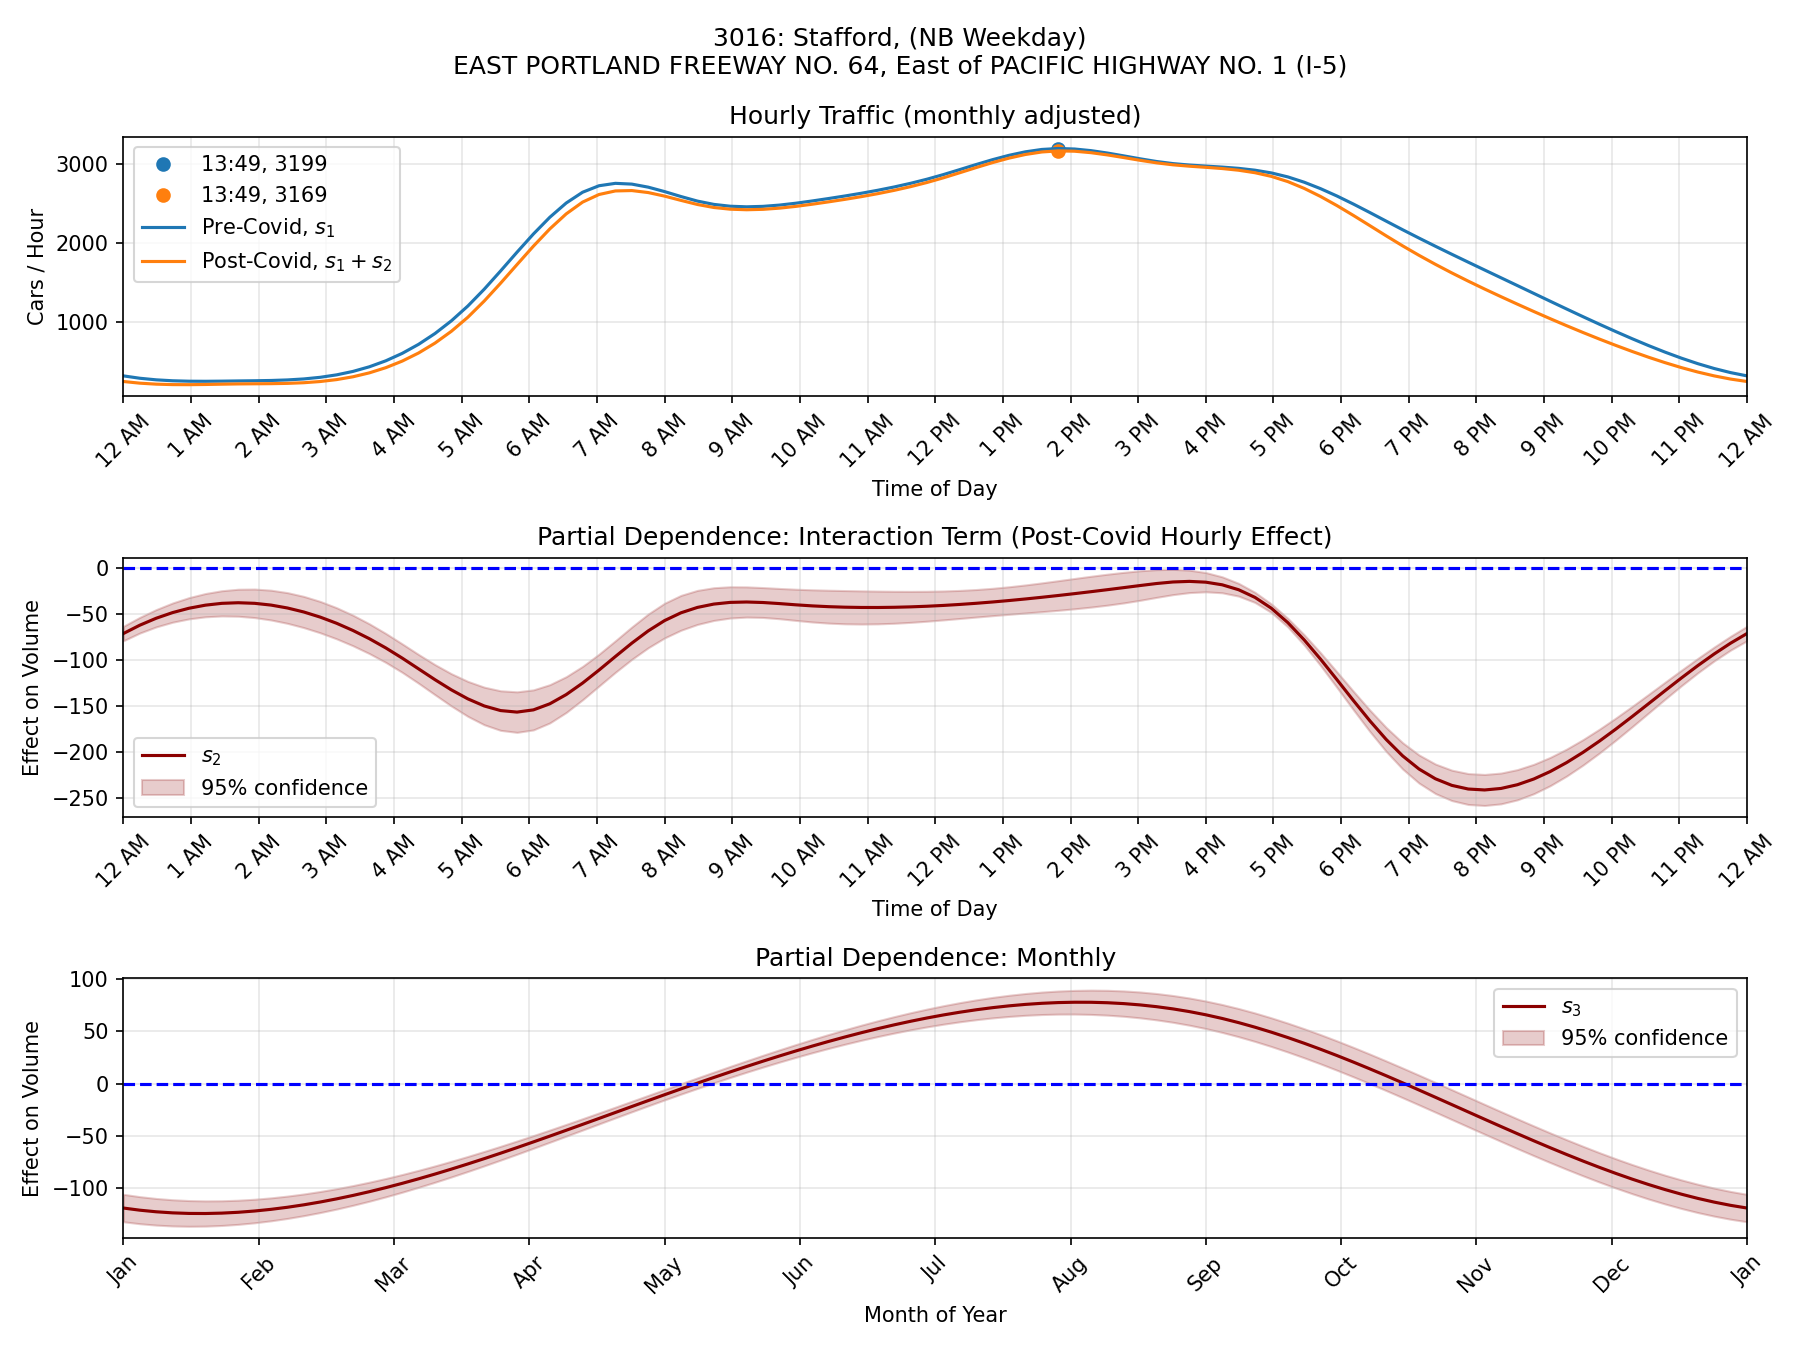
\includegraphics[width=\textwidth]{3016_Stafford_NB_Weekday_gam.png}
	\end{subfigure}
	\hfill
	\begin{subfigure}[b]{0.45\textwidth}
		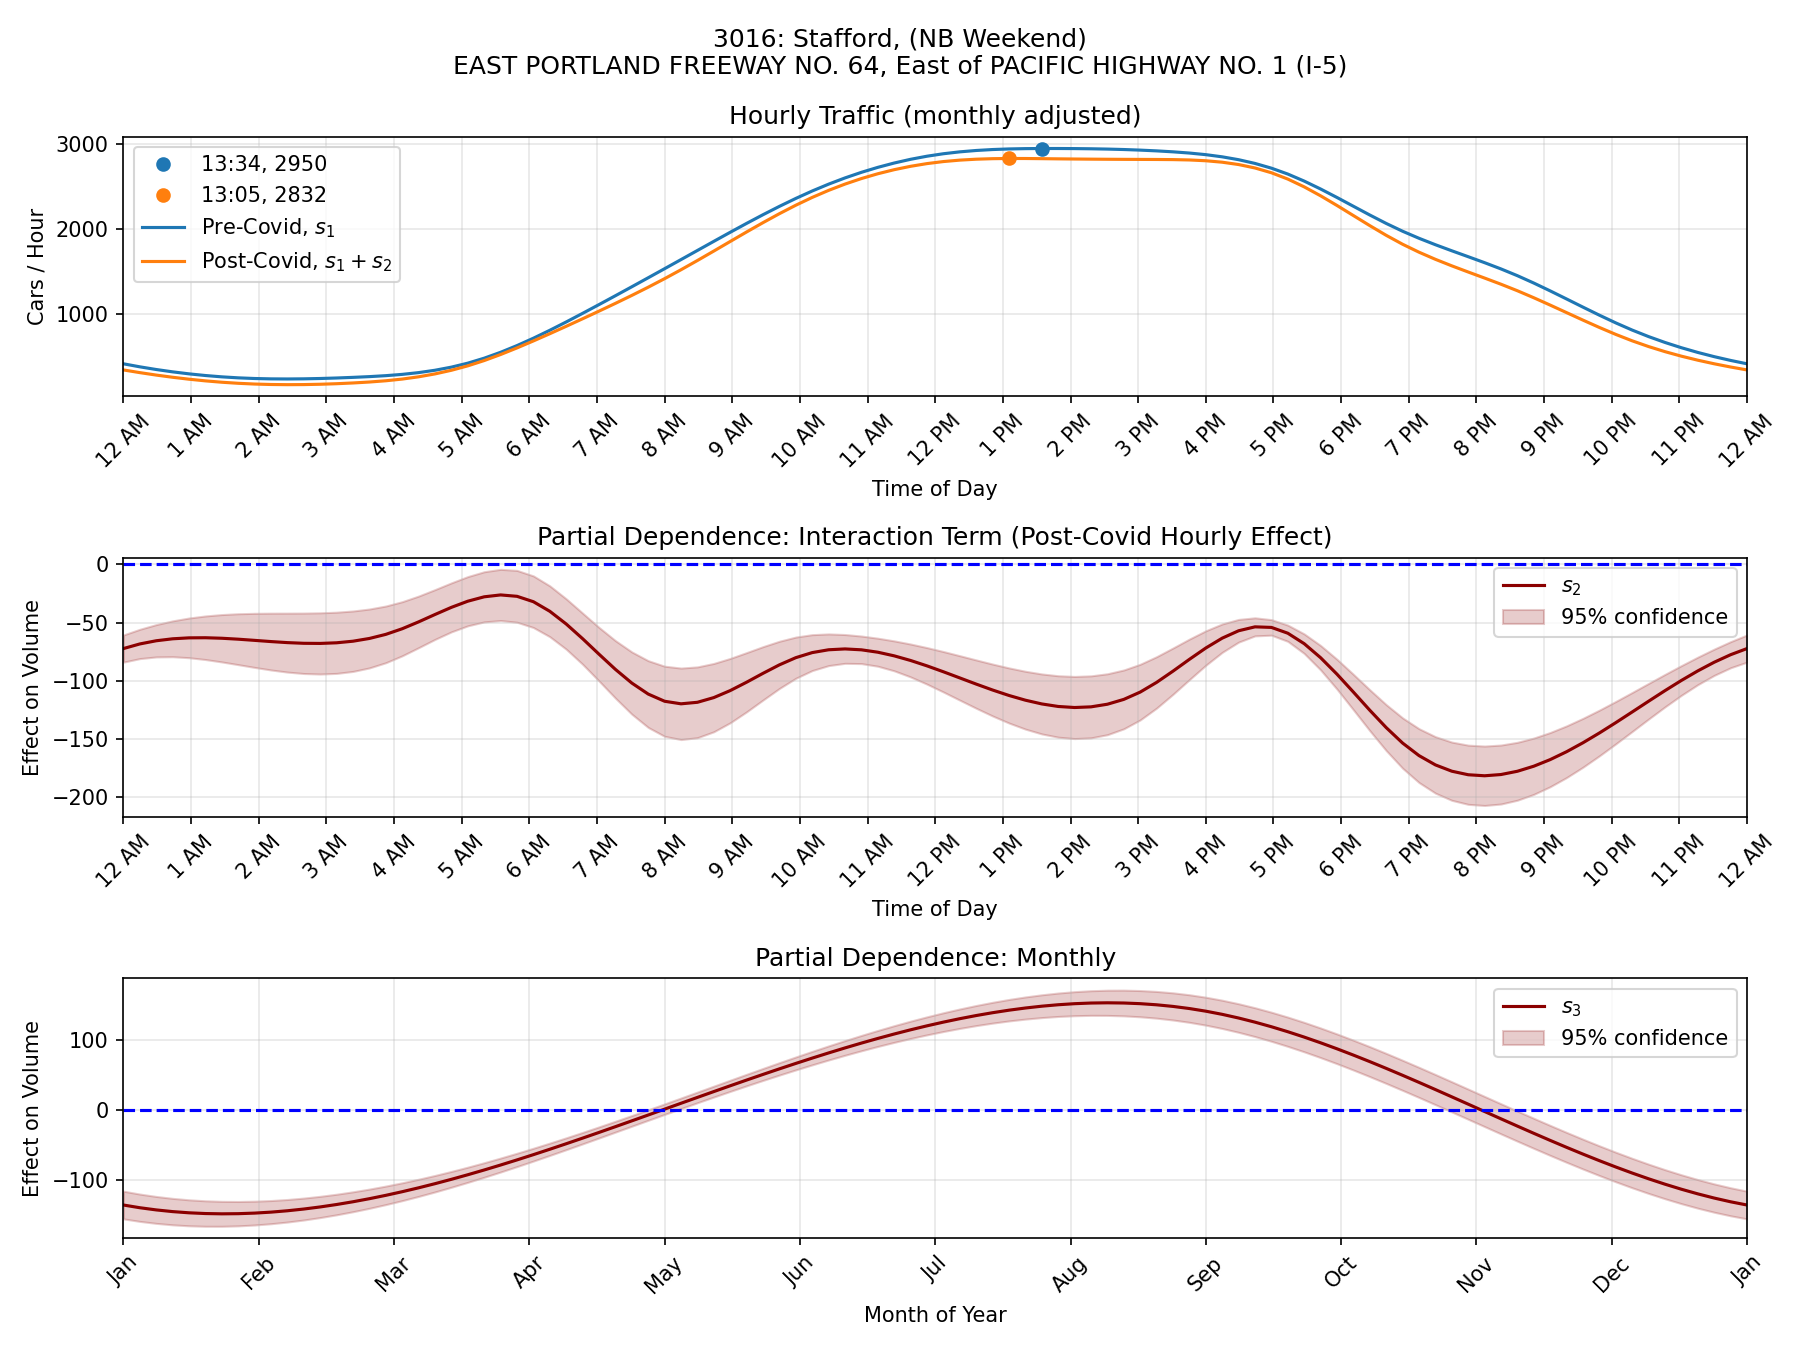
\includegraphics[width=\textwidth]{3016_Stafford_NB_Weekend_gam.png}
	\end{subfigure}

	\begin{subfigure}[b]{0.45\textwidth}
		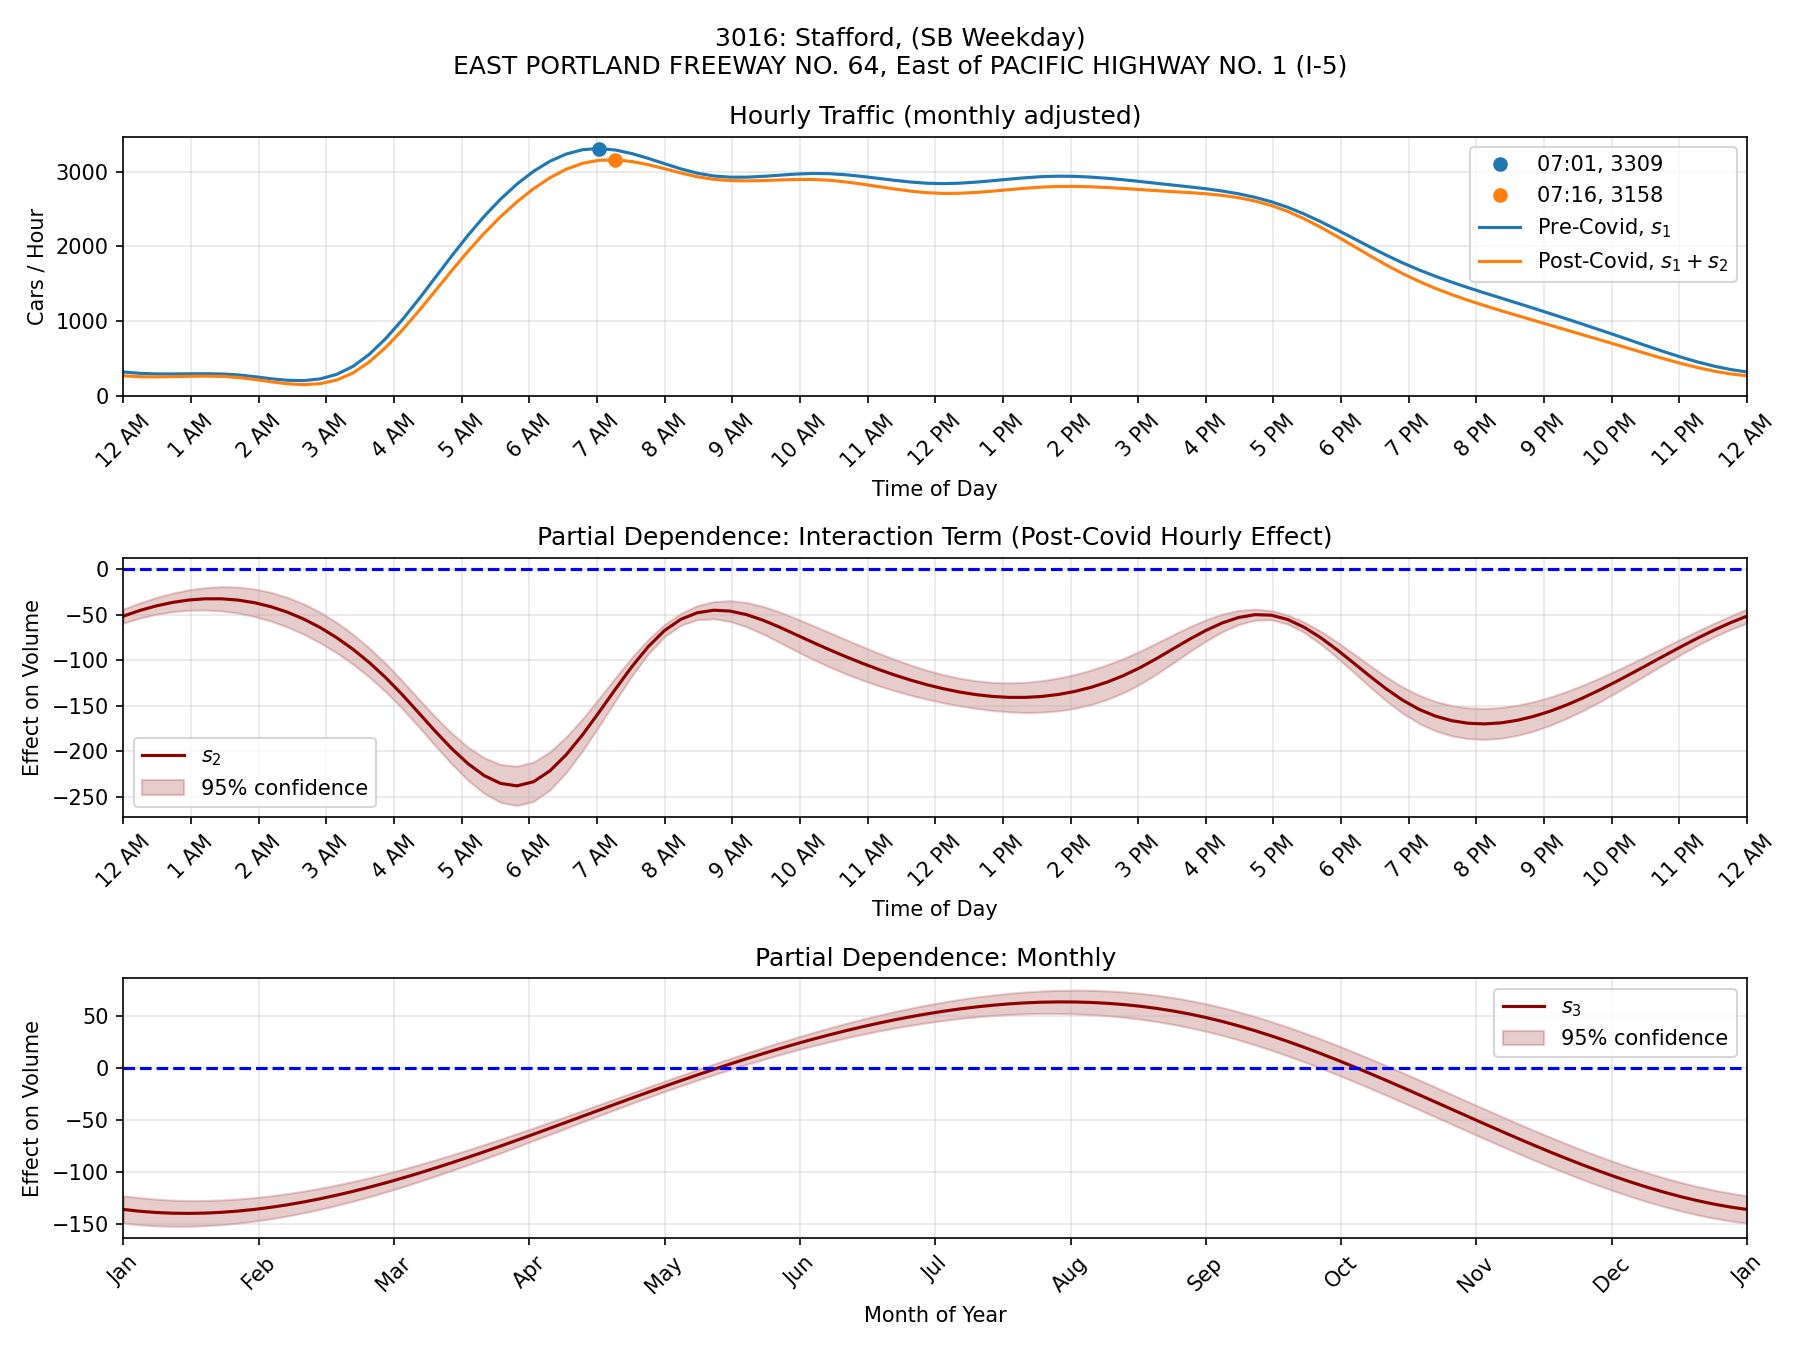
\includegraphics[width=\textwidth]{3016_Stafford_SB_Weekday_gam.png}
	\end{subfigure}
	\hfill
	\begin{subfigure}[b]{0.45\textwidth}
		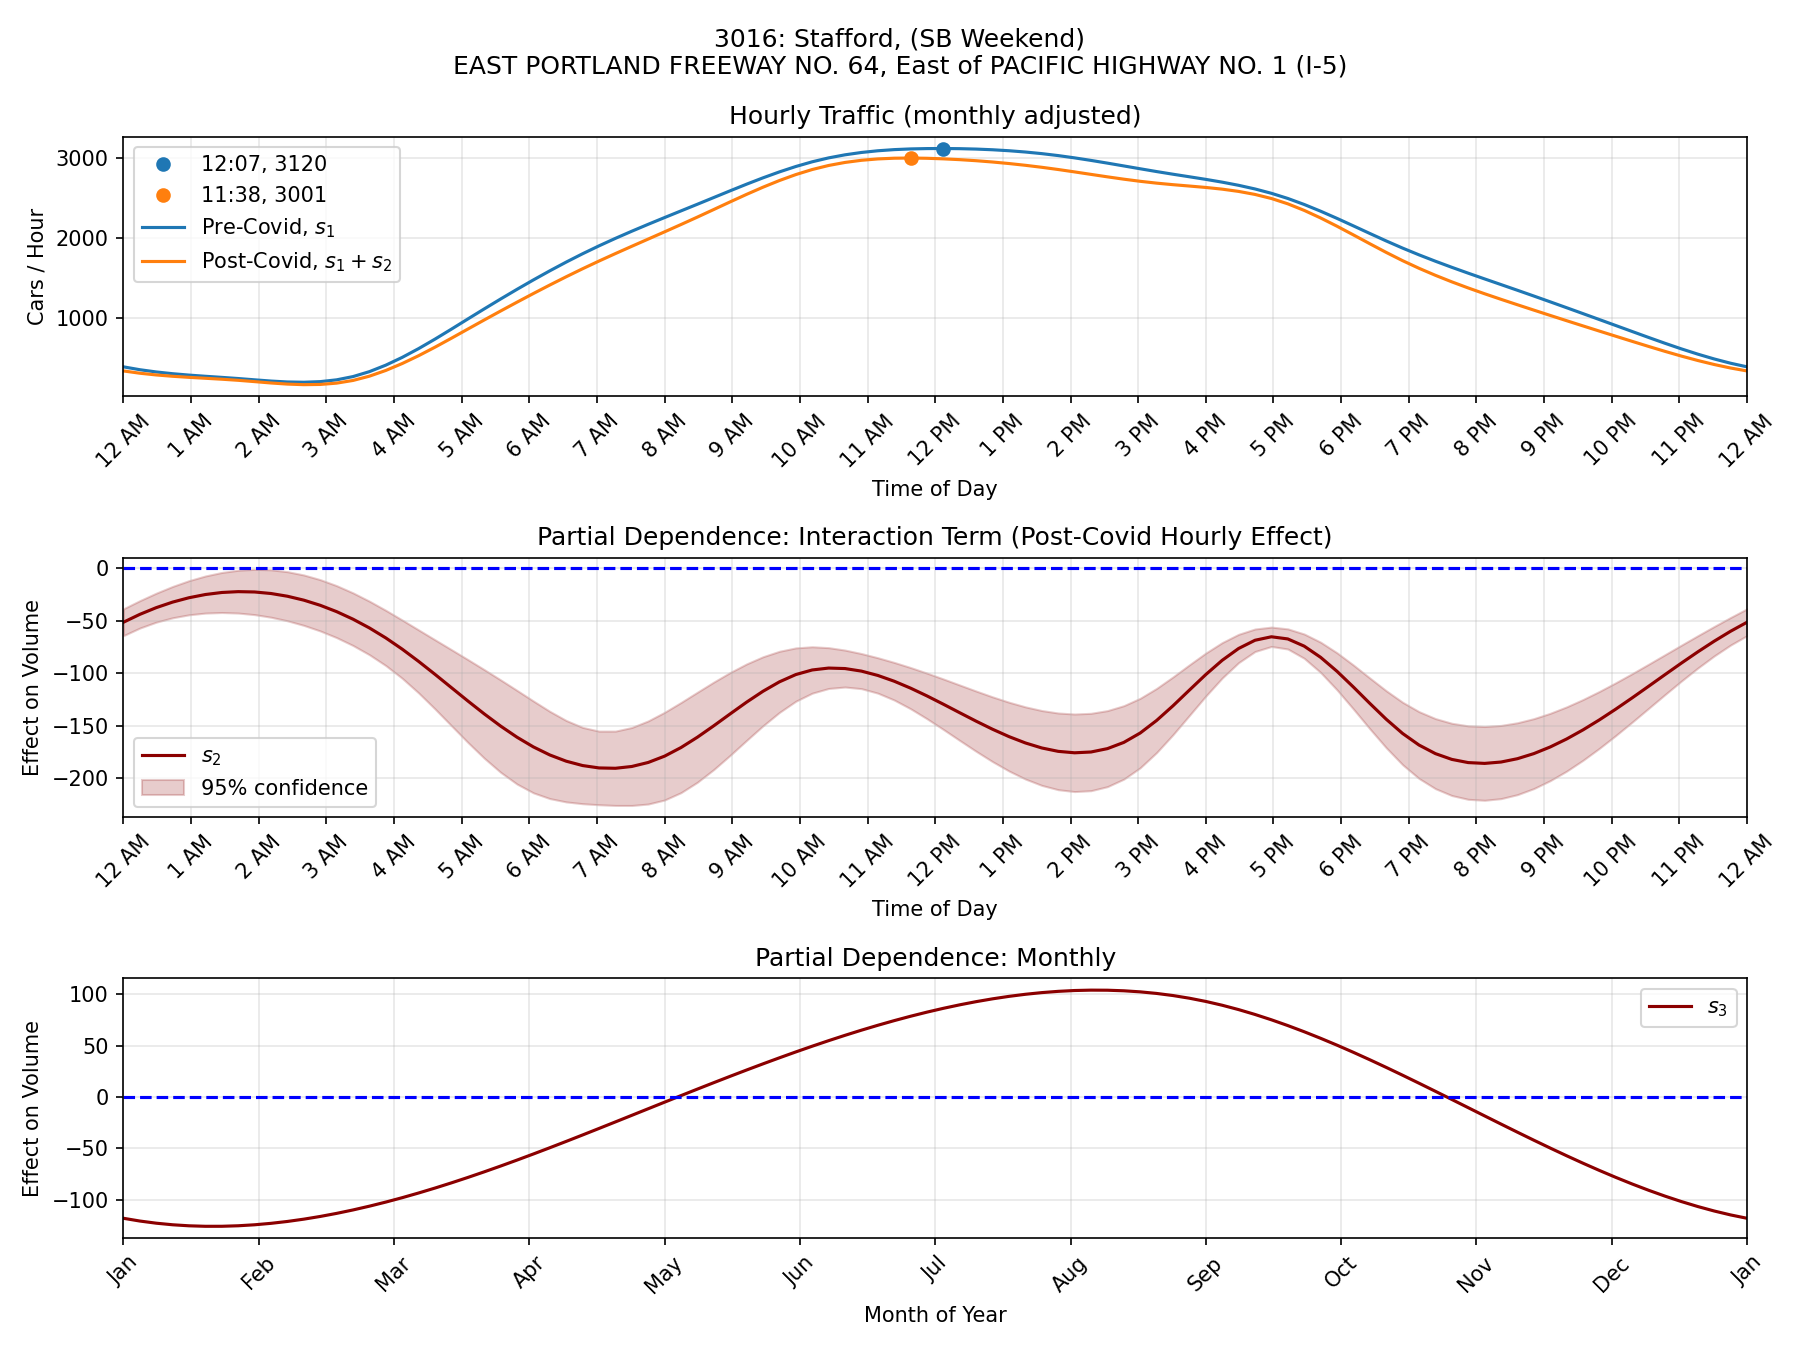
\includegraphics[width=\textwidth]{3016_Stafford_SB_Weekend_gam.png}
	\end{subfigure}
\end{figure}

\begin{figure}[H]
	\centering
	\begin{subfigure}[b]{0.45\textwidth}
		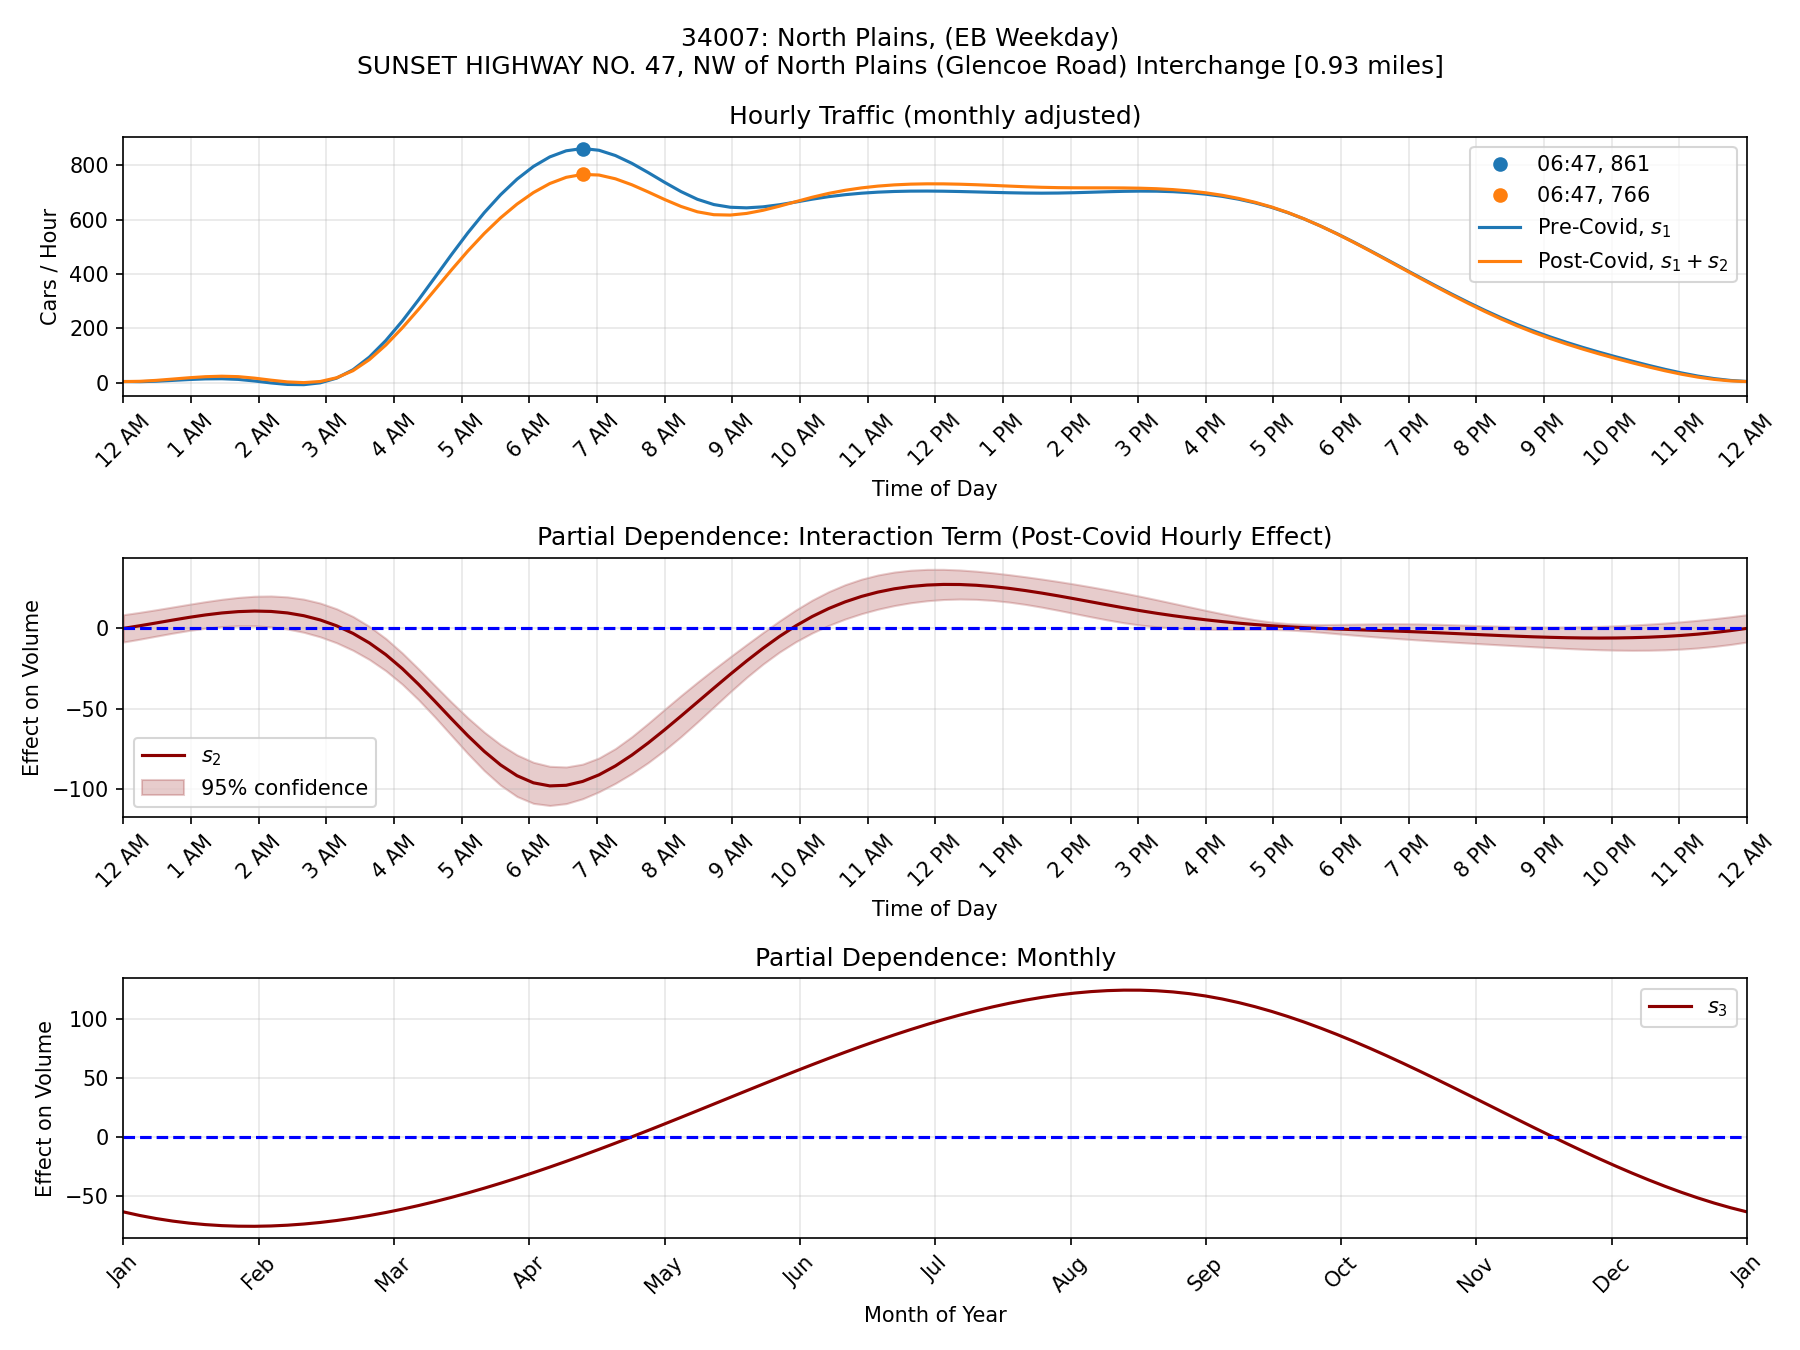
\includegraphics[width=\textwidth]{34007_North-Plains_EB_Weekday_gam.png}
	\end{subfigure}
	\hfill
	\begin{subfigure}[b]{0.45\textwidth}
		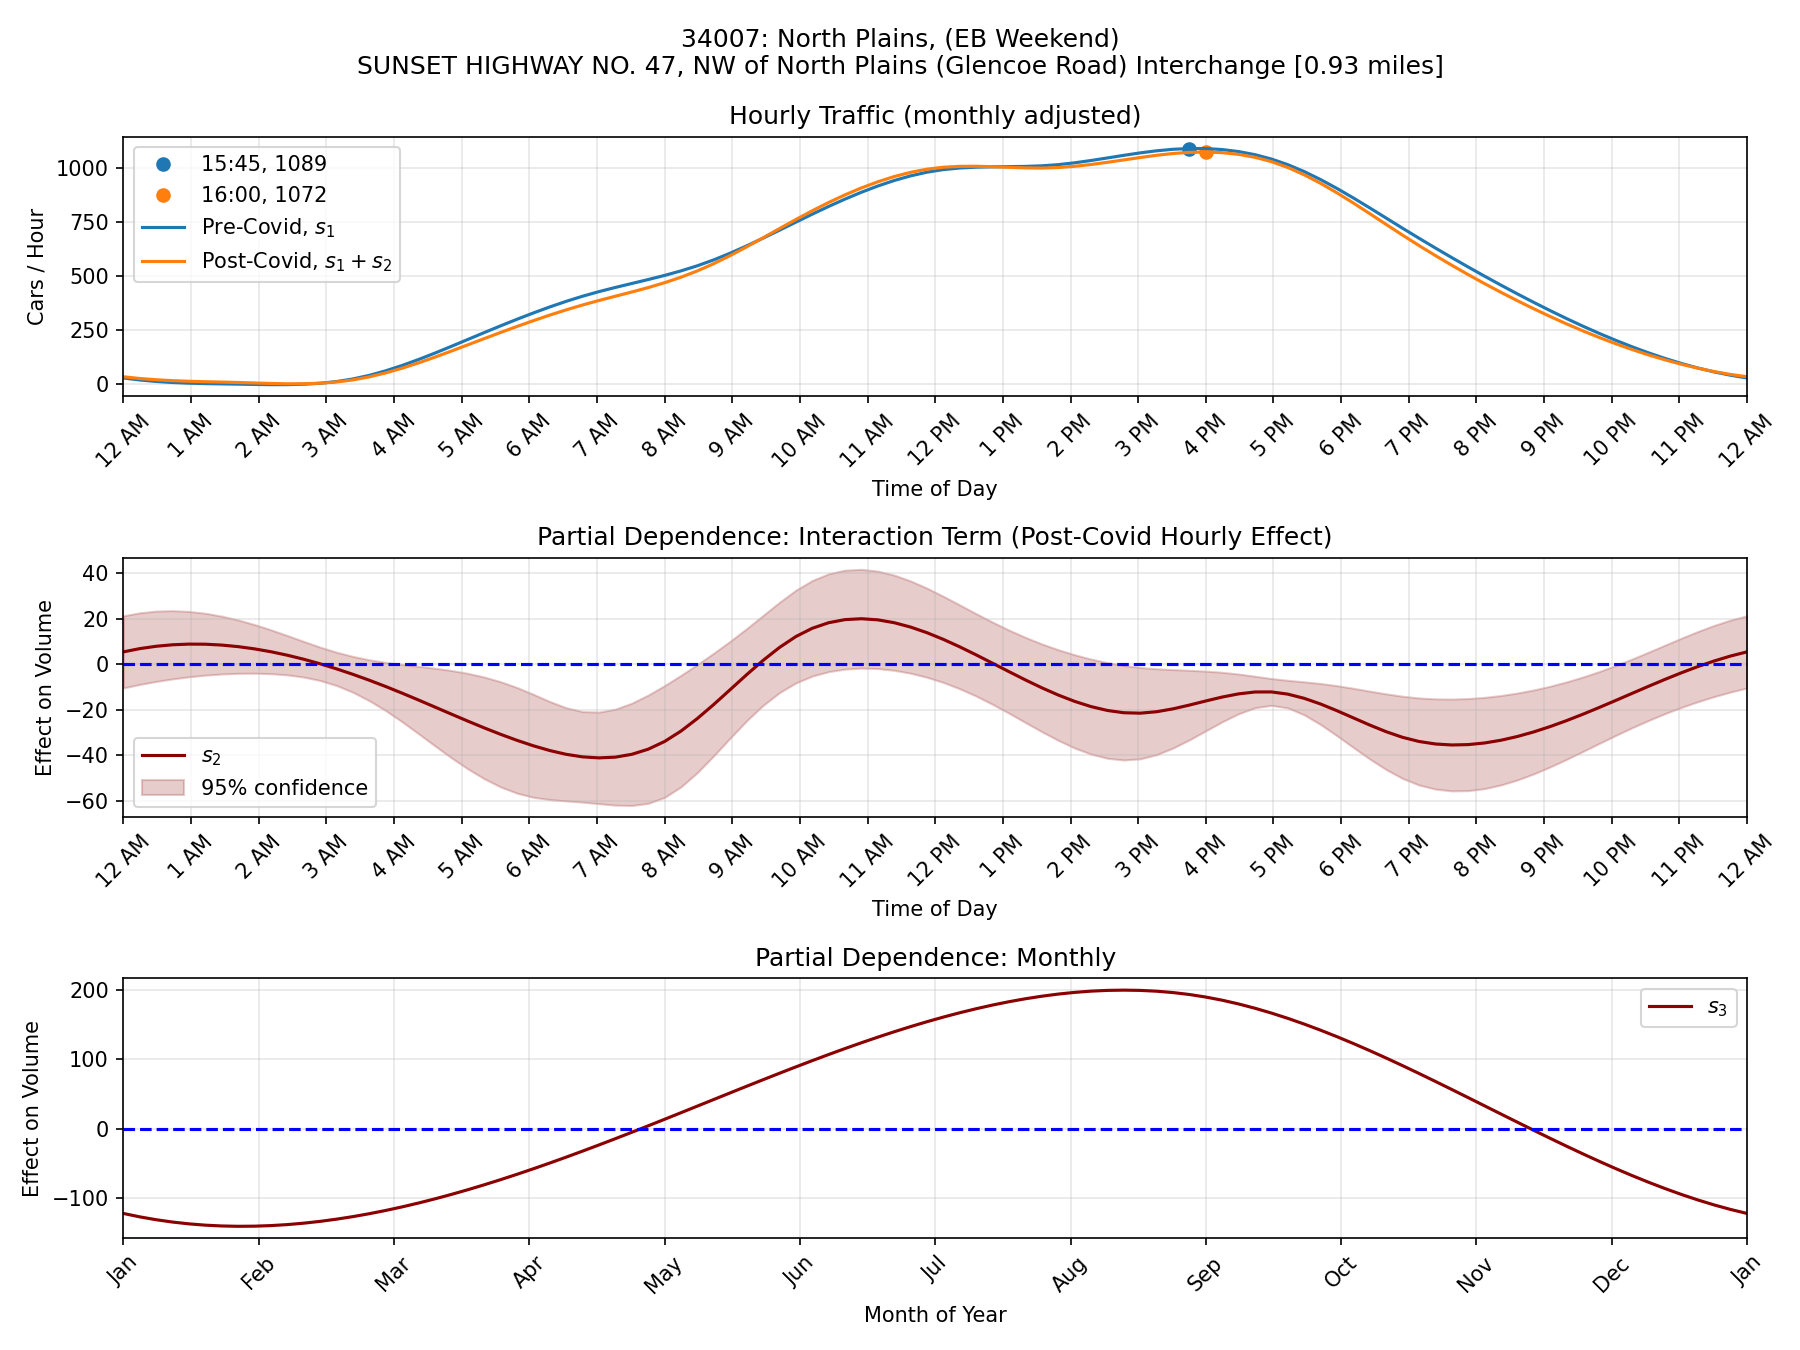
\includegraphics[width=\textwidth]{34007_North-Plains_EB_Weekend_gam.png}
	\end{subfigure}

	\begin{subfigure}[b]{0.45\textwidth}
		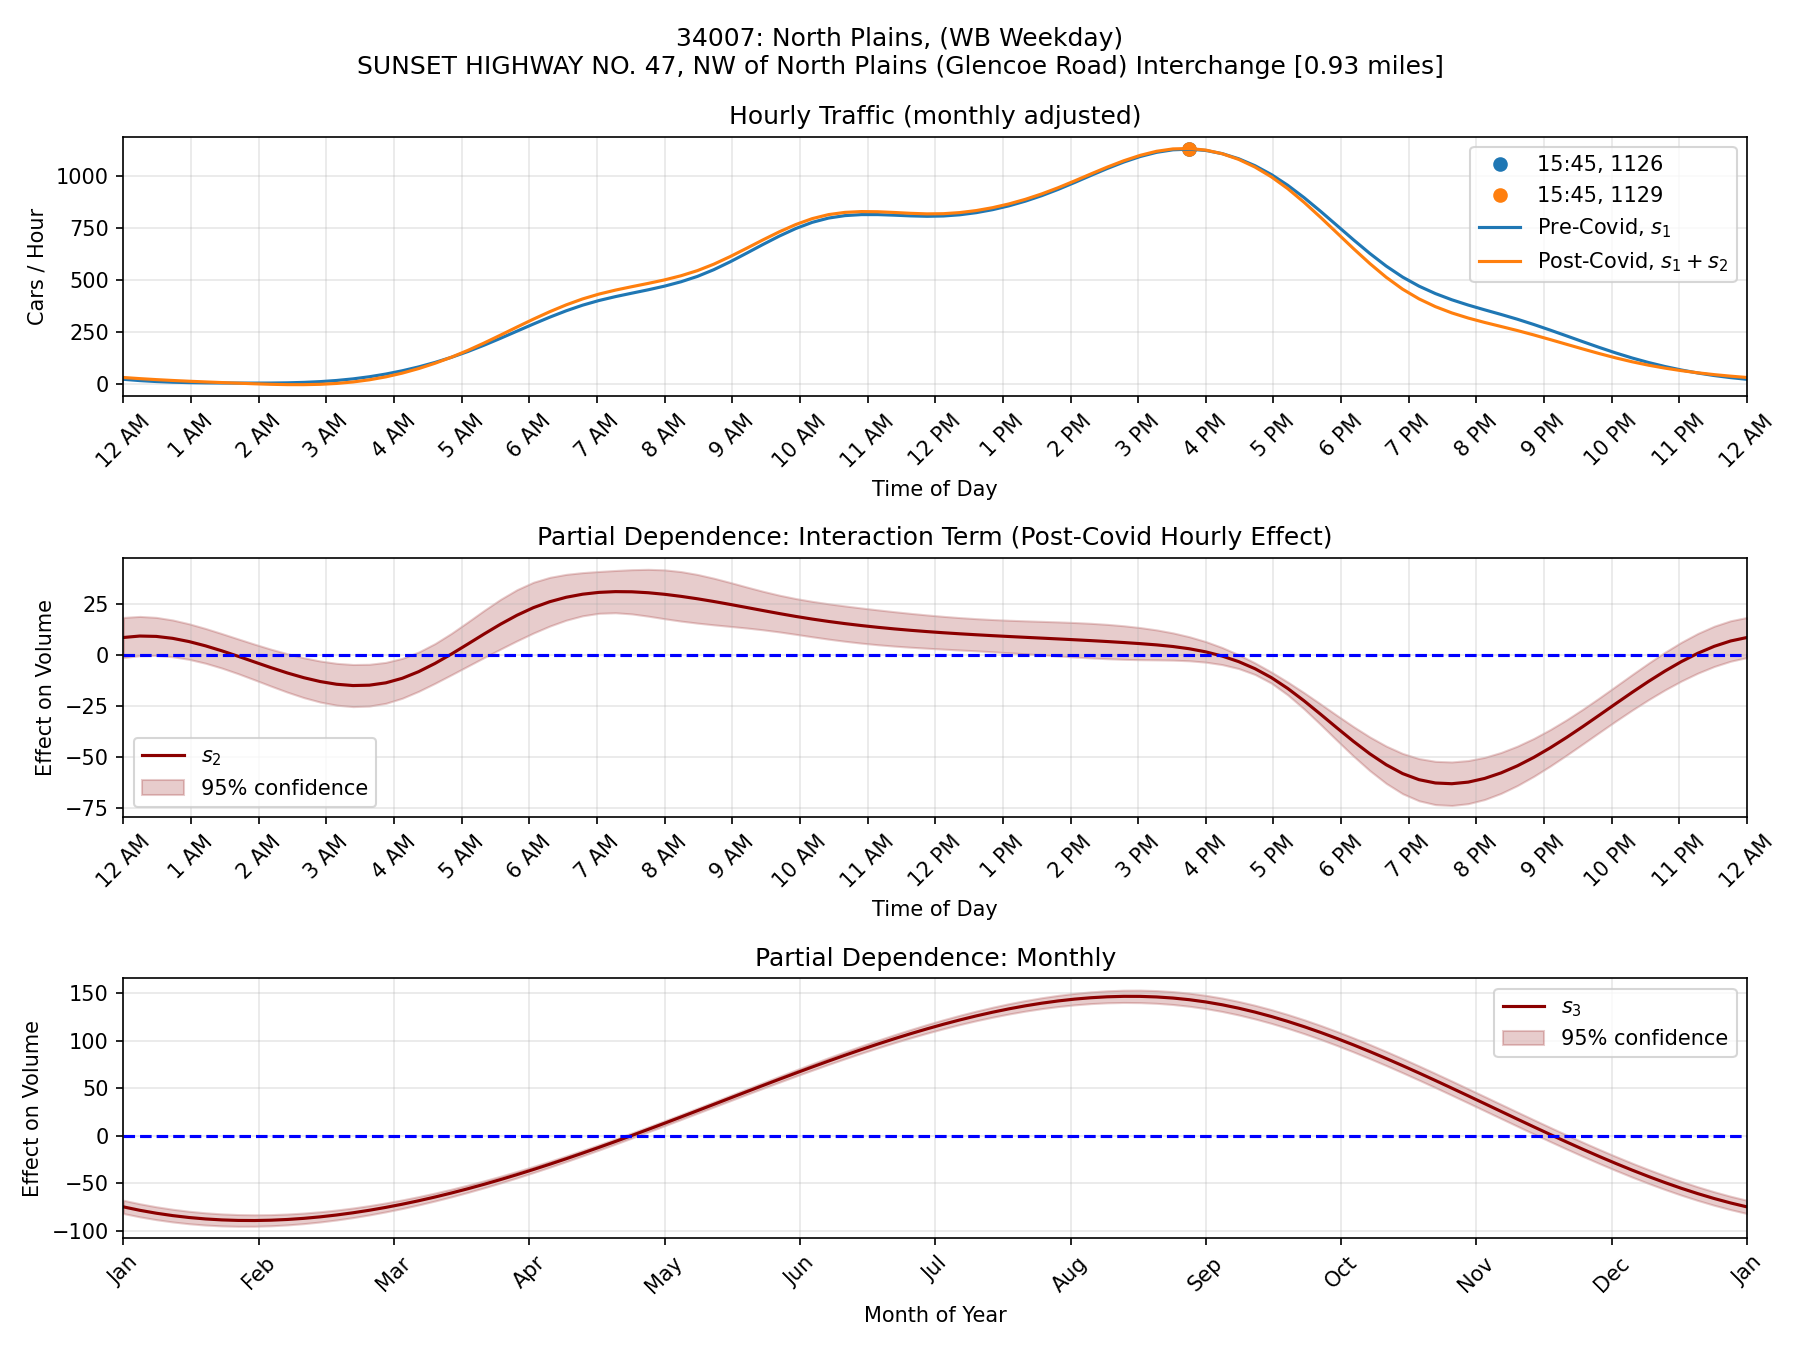
\includegraphics[width=\textwidth]{34007_North-Plains_WB_Weekday_gam.png}
	\end{subfigure}
	\hfill
	\begin{subfigure}[b]{0.45\textwidth}
		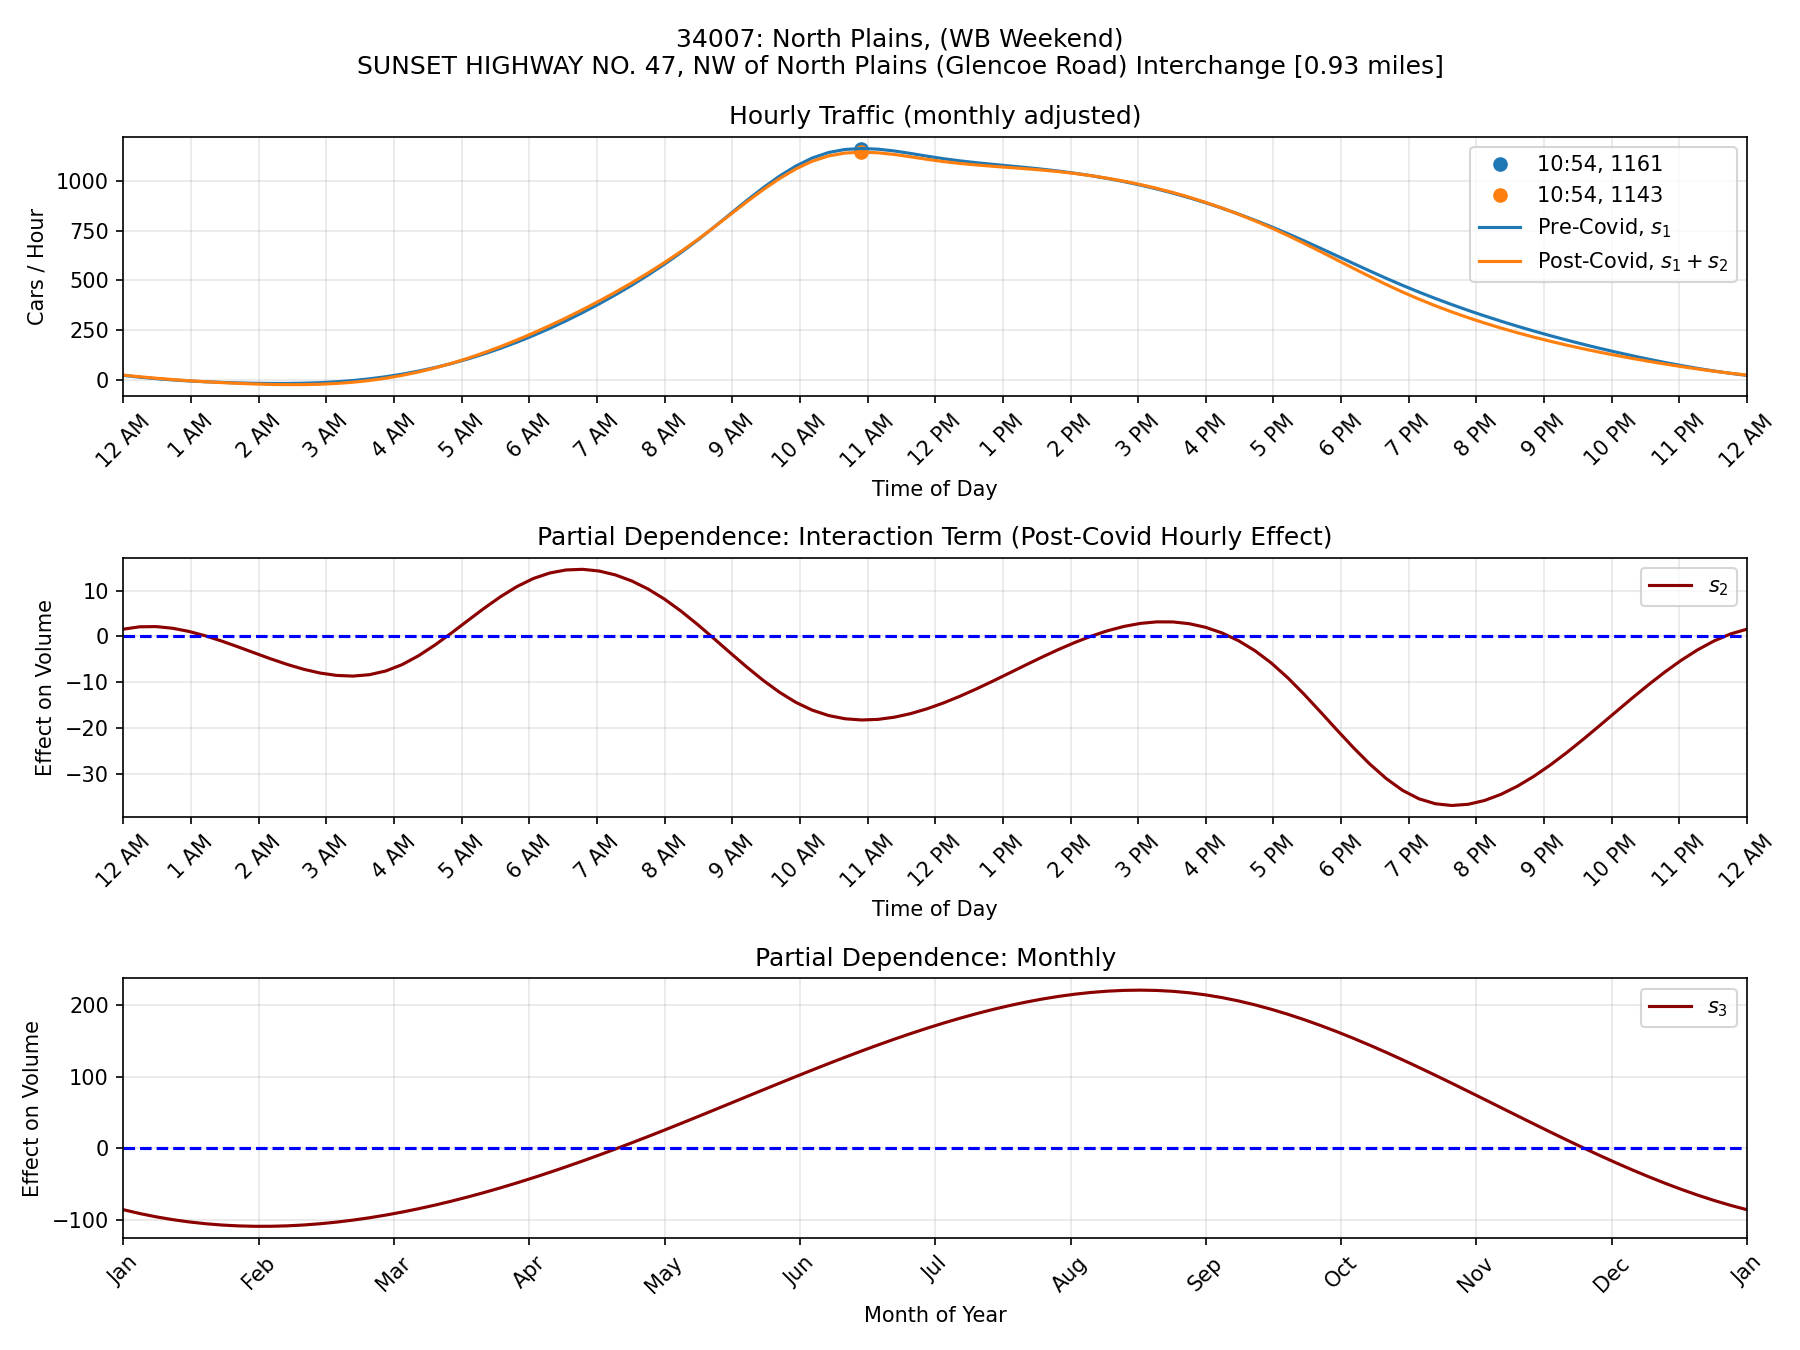
\includegraphics[width=\textwidth]{34007_North-Plains_WB_Weekend_gam.png}
	\end{subfigure}
\end{figure}

\begin{figure}[H]
	\centering
	\begin{subfigure}[b]{0.45\textwidth}
		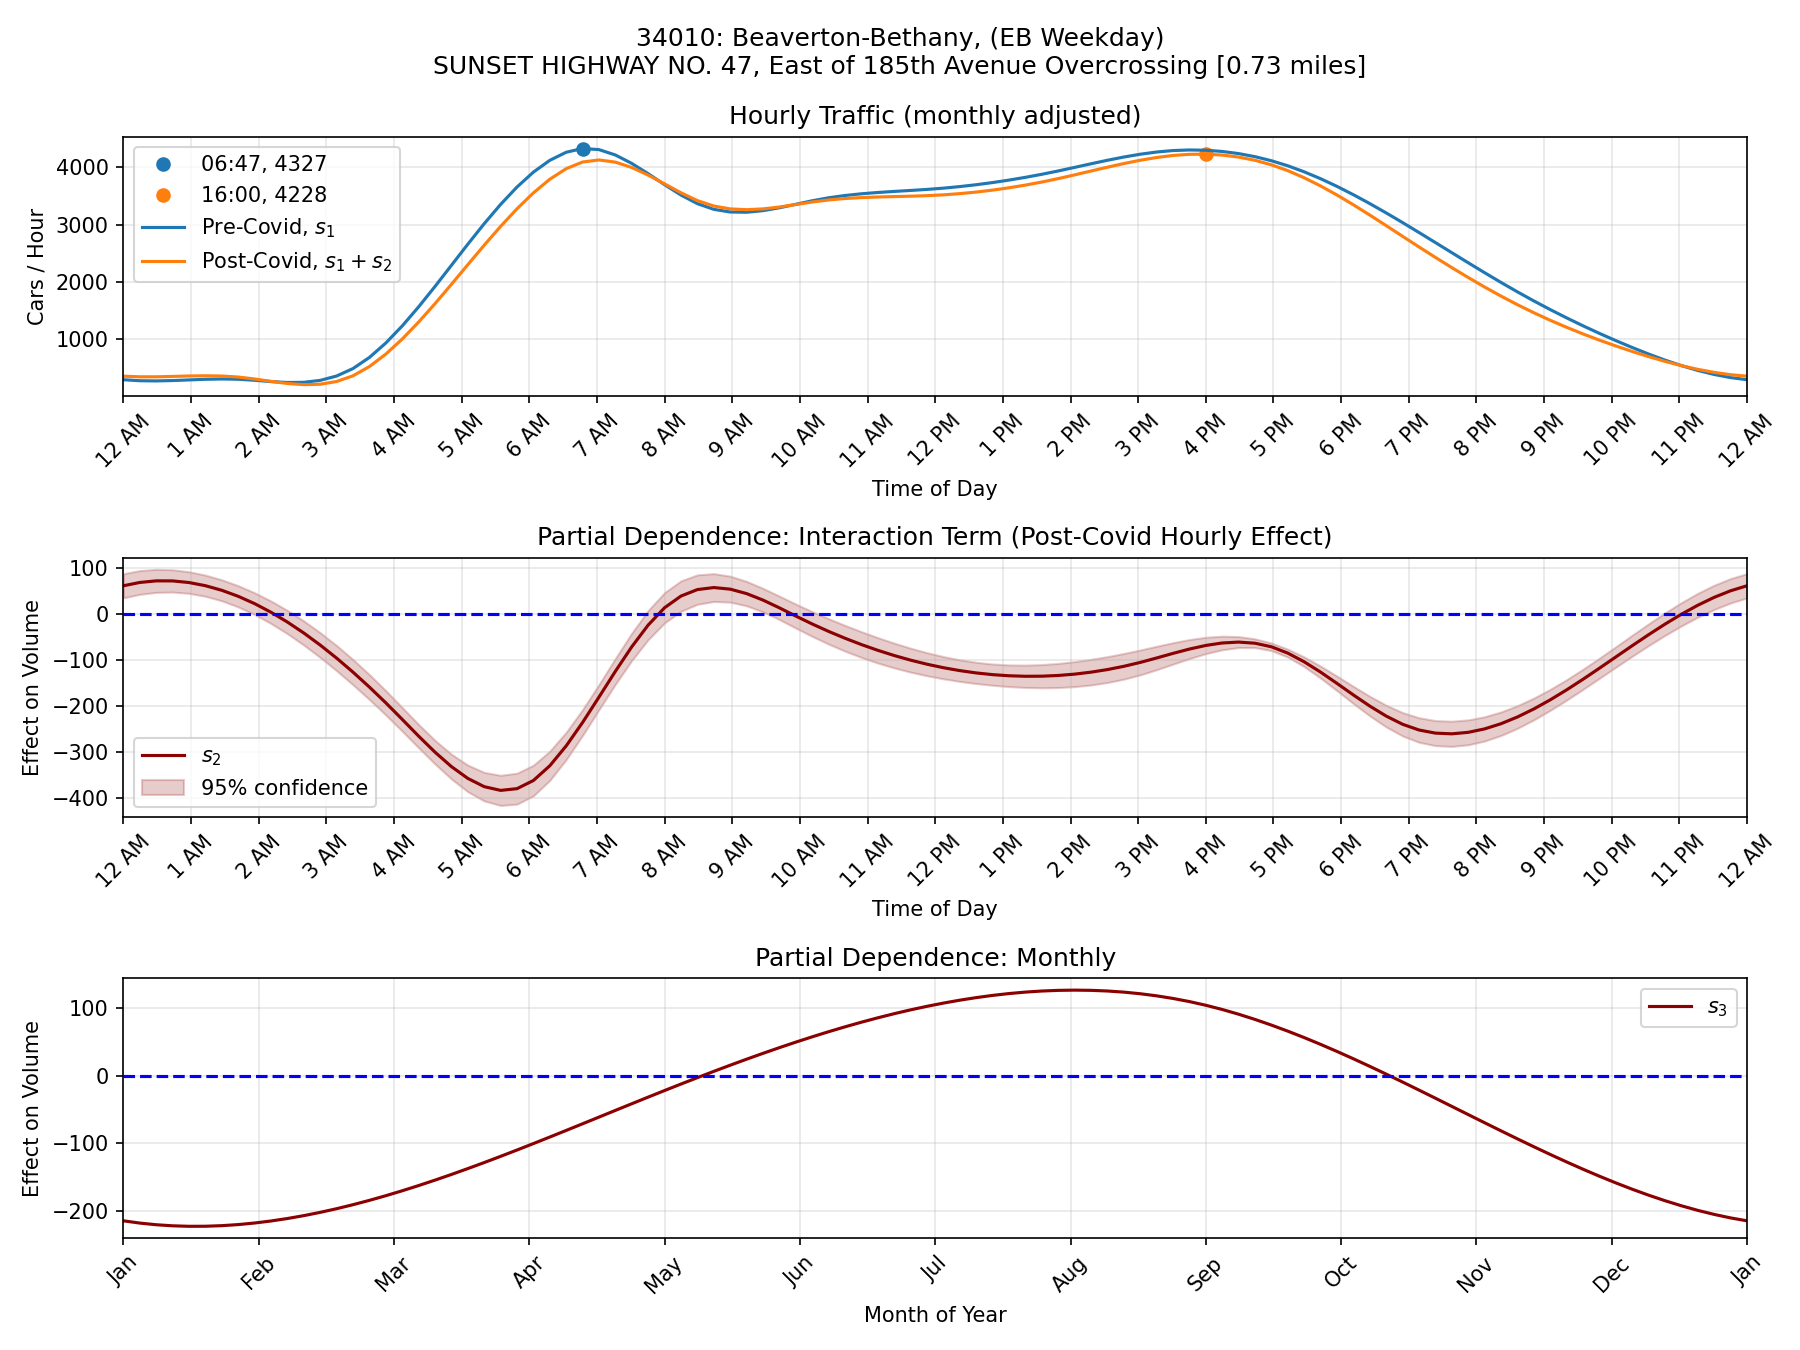
\includegraphics[width=\textwidth]{34010_Beaverton-Bethany_EB_Weekday_gam.png}
	\end{subfigure}
	\hfill
	\begin{subfigure}[b]{0.45\textwidth}
		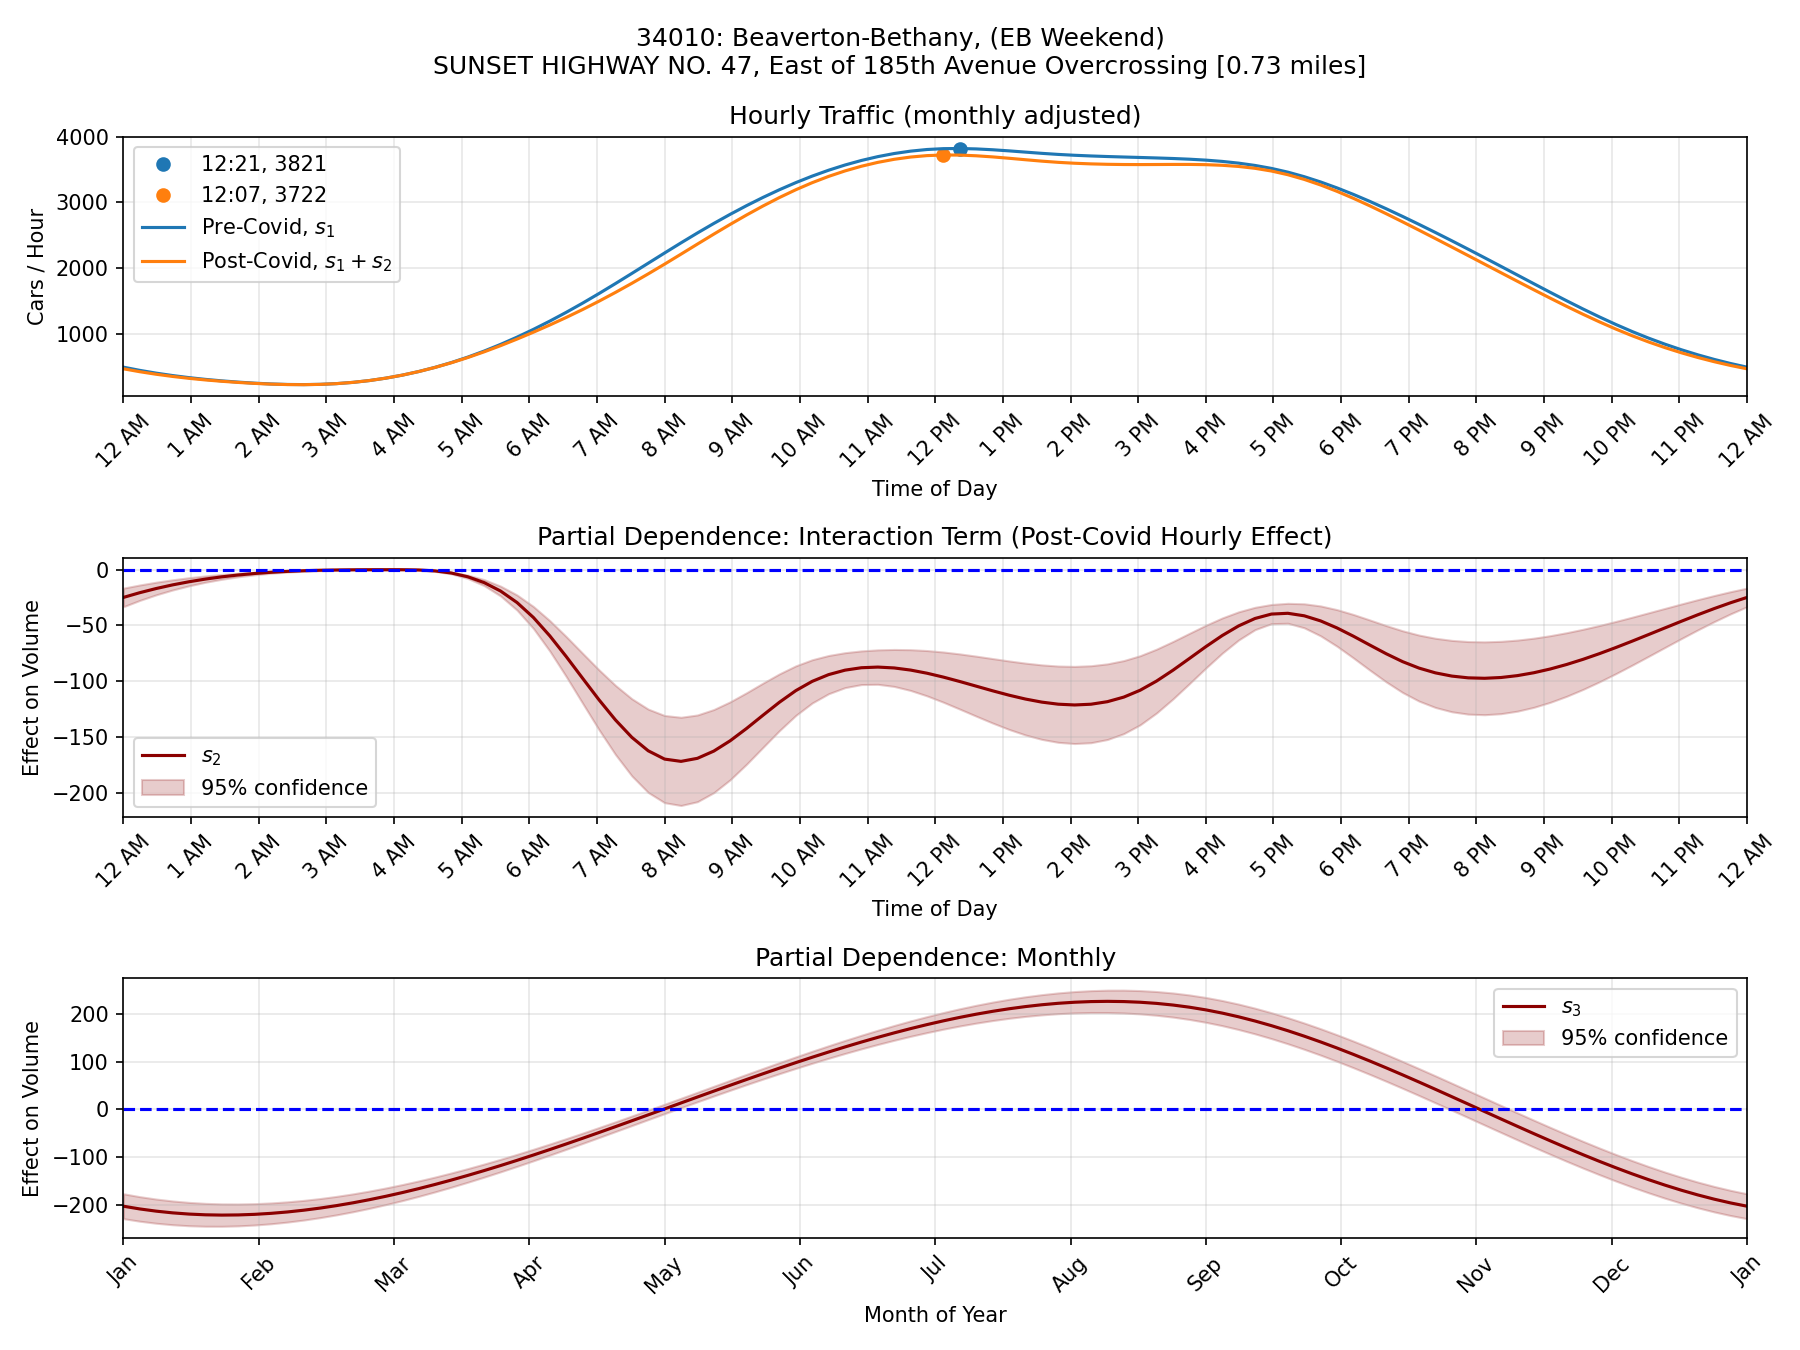
\includegraphics[width=\textwidth]{34010_Beaverton-Bethany_EB_Weekend_gam.png}
	\end{subfigure}

	\begin{subfigure}[b]{0.45\textwidth}
		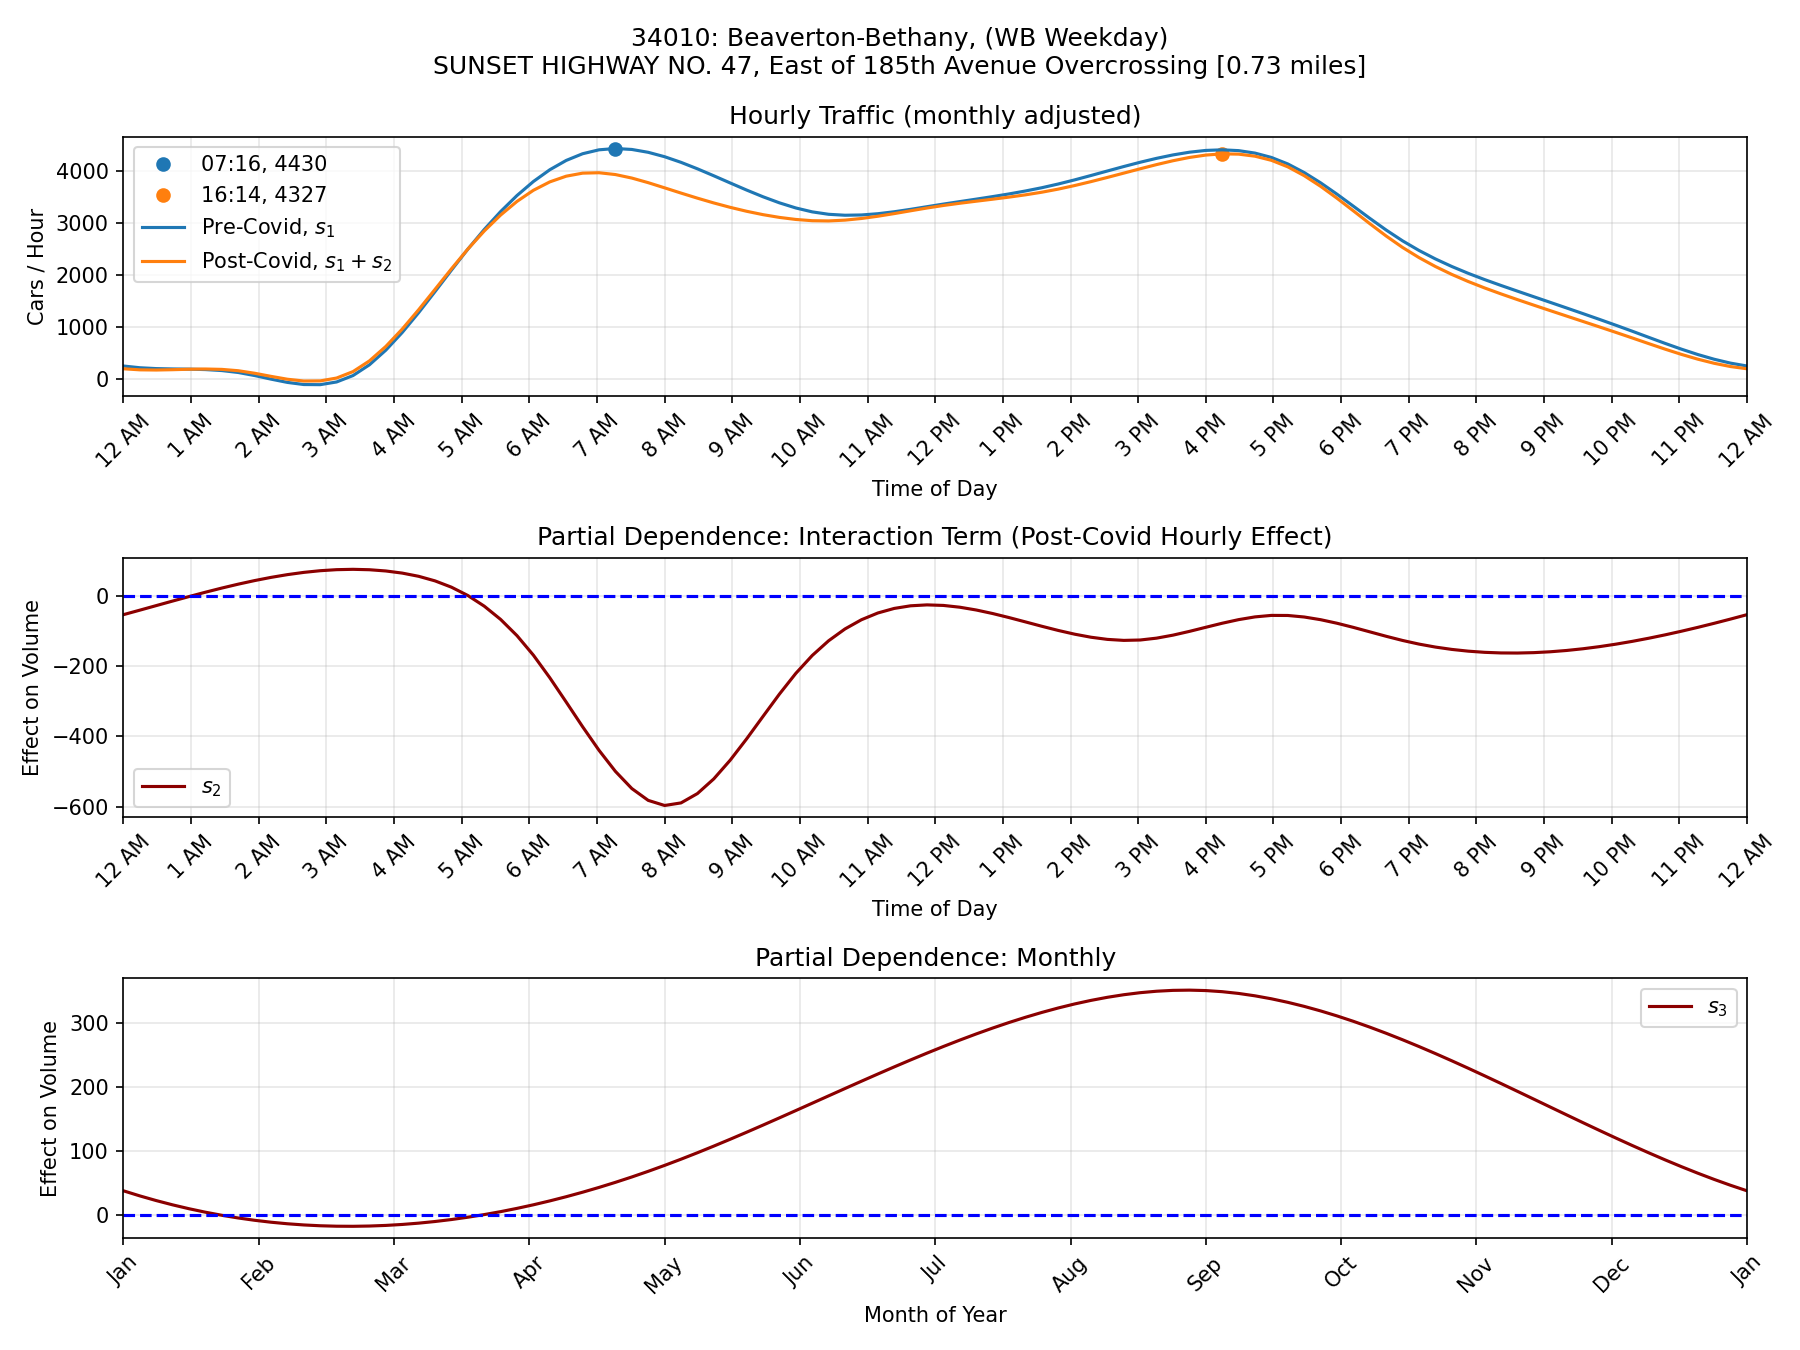
\includegraphics[width=\textwidth]{34010_Beaverton-Bethany_WB_Weekday_gam.png}
	\end{subfigure}
	\hfill
	\begin{subfigure}[b]{0.45\textwidth}
		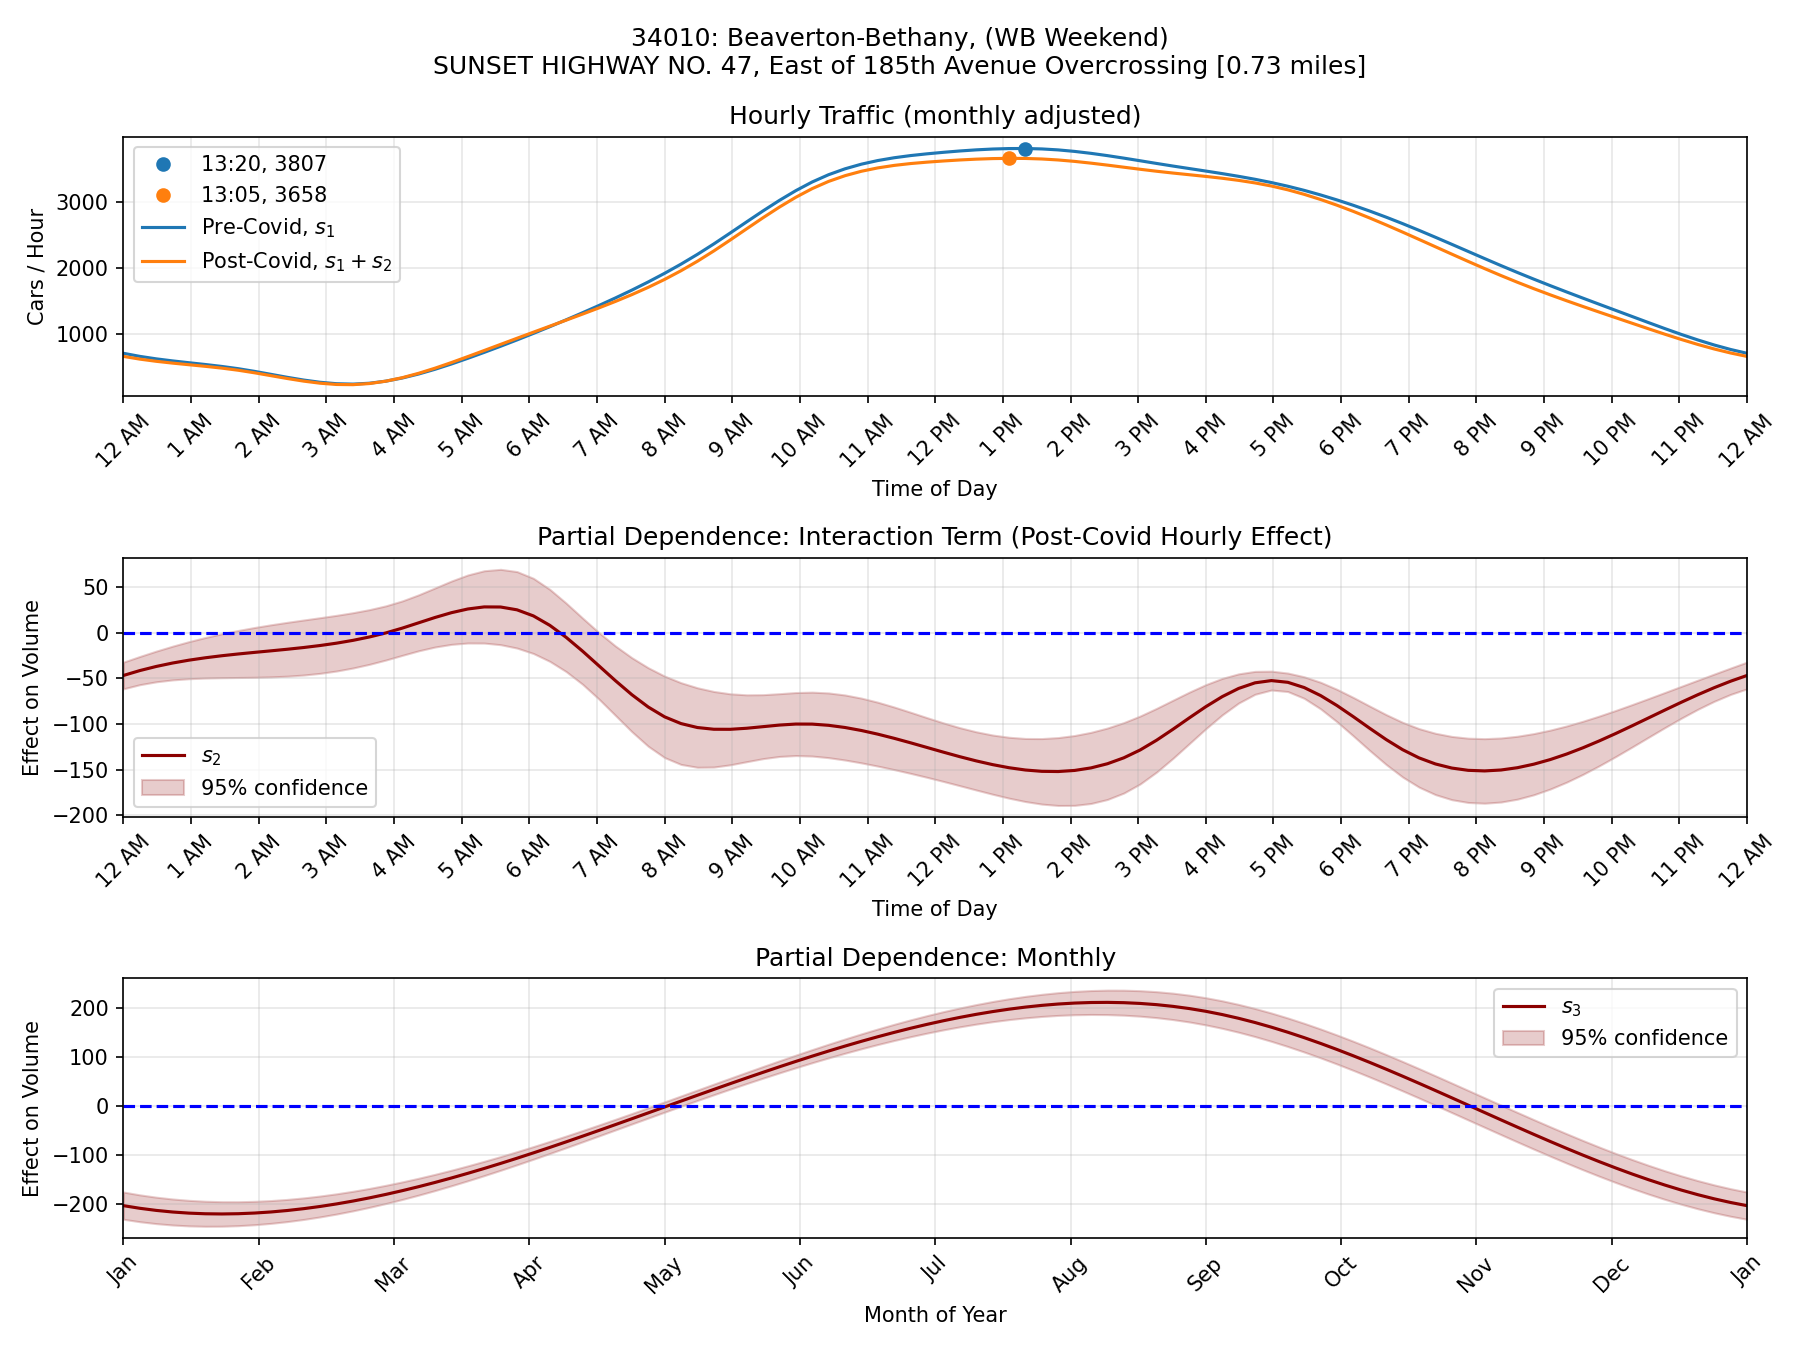
\includegraphics[width=\textwidth]{34010_Beaverton-Bethany_WB_Weekend_gam.png}
	\end{subfigure}
\end{figure}


\section{Data Availability}

\begin{figure}[H] 
    \centering
    \includegraphics[width=0.9\textwidth]{missing_data.png}
    \caption{Red indicates missing data, opacity indicates how much of that week is missing. This doesn't account for ``0'' data which is technically missing and misrepresented.}
    \label{fig:data_availability}
\end{figure}

\section{Data Issues Deep Dive by Locations} \label{app:data_issues}

These plots provide a visual for similar data presented in table \ref{tab:medians} but includes every year available in the dataset with quantile shading. Each line is the periodic cubic spline interpolation of the hourly medians/quantiles for each (location, direction, weekday/weekend) tuple. Some strange data issues become apparent in these plots, but they are almost entirely only in years we aren't concerned with in this analysis.
\begin{figure}[htbp]
	\centering
	\begin{subfigure}{0.45\textwidth}
		\includegraphics[width=\textwidth]{26001_Troutdale_EB_Weekday.png}
	\end{subfigure}
	\hfill
	\begin{subfigure}{0.45\textwidth}
		\includegraphics[width=\textwidth]{26001_Troutdale_EB_Weekend.png}
	\end{subfigure}

	\begin{subfigure}{0.45\textwidth}
		\includegraphics[width=\textwidth]{26001_Troutdale_WB_Weekday.png}
	\end{subfigure}
	\hfill
	\begin{subfigure}{0.45\textwidth}
		\includegraphics[width=\textwidth]{26001_Troutdale_WB_Weekend.png}
	\end{subfigure}
\end{figure}

\begin{figure}[htbp]
	\centering
	\begin{subfigure}{0.45\textwidth}
		\includegraphics[width=\textwidth]{26002_Vista-Ridge-Tunne_EB_Weekday.png}
	\end{subfigure}
	\hfill
	\begin{subfigure}{0.45\textwidth}
		\includegraphics[width=\textwidth]{26002_Vista-Ridge-Tunne_EB_Weekend.png}
	\end{subfigure}

	\begin{subfigure}{0.45\textwidth}
		\includegraphics[width=\textwidth]{26002_Vista-Ridge-Tunne_WB_Weekday.png}
	\end{subfigure}
	\hfill
	\begin{subfigure}{0.45\textwidth}
		\includegraphics[width=\textwidth]{26002_Vista-Ridge-Tunne_WB_Weekend.png}
	\end{subfigure}
\end{figure}

\begin{figure}[htbp]
	\centering
	\begin{subfigure}{0.45\textwidth}
		\includegraphics[width=\textwidth]{26004_Interstate-Bridge_NB_Weekday.png}
	\end{subfigure}
	\hfill
	\begin{subfigure}{0.45\textwidth}
		\includegraphics[width=\textwidth]{26004_Interstate-Bridge_NB_Weekend.png}
	\end{subfigure}

	\begin{subfigure}{0.45\textwidth}
		\includegraphics[width=\textwidth]{26004_Interstate-Bridge_SB_Weekday.png}
	\end{subfigure}
	\hfill
	\begin{subfigure}{0.45\textwidth}
		\includegraphics[width=\textwidth]{26004_Interstate-Bridge_SB_Weekend.png}
	\end{subfigure}
\end{figure}

\begin{figure}[htbp]
	\centering
	\begin{subfigure}{0.45\textwidth}
		\includegraphics[width=\textwidth]{26014_Hoyt_EB_Weekday.png}
	\end{subfigure}
	\hfill
	\begin{subfigure}{0.45\textwidth}
		\includegraphics[width=\textwidth]{26014_Hoyt_EB_Weekend.png}
	\end{subfigure}

	\begin{subfigure}{0.45\textwidth}
		\includegraphics[width=\textwidth]{26014_Hoyt_WB_Weekday.png}
	\end{subfigure}
	\hfill
	\begin{subfigure}{0.45\textwidth}
		\includegraphics[width=\textwidth]{26014_Hoyt_WB_Weekend.png}
	\end{subfigure}
\end{figure}

\begin{figure}[htbp]
	\centering
	\begin{subfigure}{0.45\textwidth}
		\includegraphics[width=\textwidth]{26016_Iowa-Street_NB_Weekday.png}
	\end{subfigure}
	\hfill
	\begin{subfigure}{0.45\textwidth}
		\includegraphics[width=\textwidth]{26016_Iowa-Street_NB_Weekend.png}
	\end{subfigure}

	\begin{subfigure}{0.45\textwidth}
		\includegraphics[width=\textwidth]{26016_Iowa-Street_SB_Weekday.png}
	\end{subfigure}
	\hfill
	\begin{subfigure}{0.45\textwidth}
		\includegraphics[width=\textwidth]{26016_Iowa-Street_SB_Weekend.png}
	\end{subfigure}
\end{figure}

\begin{figure}[htbp]
	\centering
	\begin{subfigure}{0.45\textwidth}
		\includegraphics[width=\textwidth]{26022_Lents_NB_Weekday.png}
	\end{subfigure}
	\hfill
	\begin{subfigure}{0.45\textwidth}
		\includegraphics[width=\textwidth]{26022_Lents_NB_Weekend.png}
	\end{subfigure}

	\begin{subfigure}{0.45\textwidth}
		\includegraphics[width=\textwidth]{26022_Lents_SB_Weekday.png}
	\end{subfigure}
	\hfill
	\begin{subfigure}{0.45\textwidth}
		\includegraphics[width=\textwidth]{26022_Lents_SB_Weekend.png}
	\end{subfigure}
\end{figure}

\begin{figure}[htbp]
	\centering
	\begin{subfigure}{0.45\textwidth}
		\includegraphics[width=\textwidth]{26024_Glenn-Jackson-Bridge_NB_Weekday.png}
	\end{subfigure}
	\hfill
	\begin{subfigure}{0.45\textwidth}
		\includegraphics[width=\textwidth]{26024_Glenn-Jackson-Bridge_NB_Weekend.png}
	\end{subfigure}

	\begin{subfigure}{0.45\textwidth}
		\includegraphics[width=\textwidth]{26024_Glenn-Jackson-Bridge_SB_Weekday.png}
	\end{subfigure}
	\hfill
	\begin{subfigure}{0.45\textwidth}
		\includegraphics[width=\textwidth]{26024_Glenn-Jackson-Bridge_SB_Weekend.png}
	\end{subfigure}
\end{figure}

\begin{figure}[htbp]
	\centering
	\begin{subfigure}{0.45\textwidth}
		\includegraphics[width=\textwidth]{26028_Fairview_EB_Weekday.png}
	\end{subfigure}
	\hfill
	\begin{subfigure}{0.45\textwidth}
		\includegraphics[width=\textwidth]{26028_Fairview_EB_Weekend.png}
	\end{subfigure}

	\begin{subfigure}{0.45\textwidth}
		\includegraphics[width=\textwidth]{26028_Fairview_WB_Weekday.png}
	\end{subfigure}
	\hfill
	\begin{subfigure}{0.45\textwidth}
		\includegraphics[width=\textwidth]{26028_Fairview_WB_Weekend.png}
	\end{subfigure}
\end{figure}

\begin{figure}[htbp]
	\centering
	\begin{subfigure}{0.45\textwidth}
		\includegraphics[width=\textwidth]{3011_Wilsonville_NB_Weekday.png}
	\end{subfigure}
	\hfill
	\begin{subfigure}{0.45\textwidth}
		\includegraphics[width=\textwidth]{3011_Wilsonville_NB_Weekend.png}
	\end{subfigure}

	\begin{subfigure}{0.45\textwidth}
		\includegraphics[width=\textwidth]{3011_Wilsonville_SB_Weekday.png}
	\end{subfigure}
	\hfill
	\begin{subfigure}{0.45\textwidth}
		\includegraphics[width=\textwidth]{3011_Wilsonville_SB_Weekend.png}
	\end{subfigure}
\end{figure}

\begin{figure}[htbp]
	\centering
	\begin{subfigure}{0.45\textwidth}
		\includegraphics[width=\textwidth]{3016_Stafford_NB_Weekday.png}
	\end{subfigure}
	\hfill
	\begin{subfigure}{0.45\textwidth}
		\includegraphics[width=\textwidth]{3016_Stafford_NB_Weekend.png}
	\end{subfigure}

	\begin{subfigure}{0.45\textwidth}
		\includegraphics[width=\textwidth]{3016_Stafford_SB_Weekday.png}
	\end{subfigure}
	\hfill
	\begin{subfigure}{0.45\textwidth}
		\includegraphics[width=\textwidth]{3016_Stafford_SB_Weekend.png}
	\end{subfigure}
\end{figure}

\begin{figure}[htbp]
	\centering
	\begin{subfigure}{0.45\textwidth}
		\includegraphics[width=\textwidth]{34007_North-Plains_EB_Weekday.png}
	\end{subfigure}
	\hfill
	\begin{subfigure}{0.45\textwidth}
		\includegraphics[width=\textwidth]{34007_North-Plains_EB_Weekend.png}
	\end{subfigure}

	\begin{subfigure}{0.45\textwidth}
		\includegraphics[width=\textwidth]{34007_North-Plains_WB_Weekday.png}
	\end{subfigure}
	\hfill
	\begin{subfigure}{0.45\textwidth}
		\includegraphics[width=\textwidth]{34007_North-Plains_WB_Weekend.png}
	\end{subfigure}
\end{figure}

\begin{figure}[htbp]
	\centering
	\begin{subfigure}{0.45\textwidth}
		\includegraphics[width=\textwidth]{34010_Beaverton-Bethany_EB_Weekday.png}
	\end{subfigure}
	\hfill
	\begin{subfigure}{0.45\textwidth}
		\includegraphics[width=\textwidth]{34010_Beaverton-Bethany_EB_Weekend.png}
	\end{subfigure}

	\begin{subfigure}{0.45\textwidth}
		\includegraphics[width=\textwidth]{34010_Beaverton-Bethany_WB_Weekday.png}
	\end{subfigure}
	\hfill
	\begin{subfigure}{0.45\textwidth}
		\includegraphics[width=\textwidth]{34010_Beaverton-Bethany_WB_Weekend.png}
	\end{subfigure}
\end{figure}


%\bibliography{references}
\end{document}

